\documentclass[11pt]{article}
\usepackage{geometry}
% Math packages.
\usepackage{amsmath,amssymb,amstext,amsfonts}
% Add figures.
\usepackage{graphicx}
\usepackage{float}

% Metadata
\author{Jarod Klion}
\title{Root-Finding Methods}

\begin{document}

\maketitle

\section{Executive Summary}

In this report, we consider the accuracy for the bisection, Newton, and fixed-point root-finding methods of a function. Analytic derivations are confirmed by loglog plots of the function values achieved at each iteration. Results are obtained and discussed for two functions: $f(x) = xe^{-x} - 0.06064$ and $g(x) = x^3 - x - 6$.

\section{Statement of the Problem}

The numerical approximation of roots of a function is important in scientific and mathematical-computing applications, e.g., solving any equation defined by continuous functions. Root-finding algorithms, which often depend on a parameter, $x_0$, can be used to find these approximations, and the iterations required, or time taken, to converge often depends on this value. We will analyze the accuracy and convergence properties for the bisection, Newton, and fixed-point method approximations, respectively:
\begin{enumerate}
	\item Bisection: $m = \frac{a + b}{2}$
	\item Newton's: $x_{k+1} = x_k - \frac{f(x_k)}{f'(x_k)}$
	\item Fixed-point: $x_{k+1} = \phi(x_k)$
\end{enumerate}


\section{Description of the Algorithms and Implementation}

The root-finding methods each are translated directly into their respective functions in \textbf{Python}. The bisection method accepts four arguments: (1) a function, $f$, (2) a starting left bound, $a$, (3) a starting right bound, $b$, and (4) a value, \emph{tol}. Newton's method also accepts four arguments: (1) a function, $f$, (2) the function's derivative, $f'$, (3) a starting value $x_0$, and (4) a value, \emph{tol}. Lastly, the fixed-point method accepts three arguments: (1) a function, $f$, (2) a starting value $x_0$, and (3) a value, \emph{tol}. For example, if a function, \textbf{func}, is previously defined, then \textbf{bisection(func, 1, 10, 10e-6)} returns the bisection method's approximation of a root, if one exists, of \textbf{func} in the interval $[1, 10]$ with accuracy to the order of $10^{-6}$.

\section{Description of the Experimental Design and Results}

For each root-finding method, function, and starting values, the order of the accuracy is estimated by plotting, in logscale, the obtained error against each iteration step, $k$, as well as the function value, $f(x_k)$, at each x-value achieved at the $k$-th iteration step,  $x_k$. This yields as many values as was required to reach the desired tolerance values. We will begin the discussion of our results for the methods as they relate to $f(x)$ first, then the results obtained for $g(x)$ following that.

For the bisection method on $f(x)$, the interval sizes, $b - a$, versus the iteration step, $k$ were plotted with results for each root shown in Figures \ref{fig:bisec_f1} and  \ref{fig:bisec_f2}, respectively. We can see the general shape of the curve and the amount of iterations taken are about the same when finding either root. In Figures \ref{fig:newton_f_0.0}, \ref{fig:newton_f_0.99}, \ref{fig:newton_f_1.1}, \ref{fig:newton_f_4.0}, and \ref{fig:newton_f_6.0}, $f(x_k)$ versus $x_k$ are plotted against each other for all $k$ obtained through Newton's method. We immediately notice in figures \ref{fig:newton_f_0.99} and \ref{fig:newton_f_1.1}, which use initial x-values, $x_0$, that are close to undefined values for Newton's method - $f'(x_0) = 0$ - that the values of both $x_k$ and $f(x_k)$ are many magnitudes higher than what was obtained in Figure \ref{fig:newton_f_0.0} where $x_0 = 0.0$. In Figures \ref{fig:fixed_f_0.0} and \ref{fig:fixed_f_4.5}, $\phi(x_k)$ versus $x_k$ are plotted against each other as well as $y=x$ to see each iteration of the fixed-point method. We see that for either root, it takes only a few points before converging to the root.

For the bisection method on $g(x)$, the interval size, $b-a$, versus the iteration step, $k$, was plotted with results for the root shown in Figure \ref{fig:bisec_g}. We can see that it once again takes the same shape as the $f(x)$ case but with slightly more iterations required for convergence. Additionally, in Figure \ref{fig:bisec_g_err}, the relative error at each step was plotted against the iteration step, and we can see that there is a "zig-zag" pattern between the consecutive error values, which is more than likely due to how the bisection method chooses a testing interval. Next, in Figures \ref{fig:newton_g_0.0}, \ref{fig:newton_g_0.57735}, \ref{fig:newton_g_1.0}, and \ref{fig:newton_g_sqrt3}, $g(x_k)$ versus $x_k$ are plotted for all $k$ obtained when using Newton's method to find the root of $g(x)$. We see in each of the listed figures that as we approach the actual root, $x = 2$, we appear to require fewer and fewer iterations to converge to the root. In Figures \ref{fig:fixed_g_0.0}, the fixed-point function values, $\phi(x_k)$, versus $x_k$ are plotted against each other for a starting value of $x_0 = 0.0$. We see that for the fixed-point method, only about four iterations are required to converge to the root within the desired accuracy.

In Tables \ref{tab:bisec_f}, \ref{tab:newton_f}, and \ref{tab:fixed_f}, the visually estimated iterations nearly match the actual iterations each root-finding method took to converge for the roots of $f(x)$. In Table \ref{tab:bisec_f}, the initial $[a,b]$'s were chosen because it can be easily seen that $f(x \leq 0) < 0$, so $a = 0$ was chosen with $b=1$ chosen as to not cover that wide of an interval in the case of multiple roots. We notice in Table \ref{tab:newton_f} that we receive an error in the case of $x_0 = 1.0$. This is so because the derivative of $f$, which is the divisor in Newton's method, is $f'(x) = e^{-x}(1-x)$, which takes a value of zero at that initial x-value --- $f'(x_0 = 1.0) = 0$ --- leaving us with an error by trying to divide by zero. Additionally, we find that Newton's method, especially in the case of $x_0 = 0.0$ and $x_0 = 4.0$ for the first and second roots, respectively, converges in the fewest total iterations. This is not the case for Newton's method with $x_0 = 0.99$ or $x_0 = 1.1$ as they are near the derivative's 0 value, i.e., $f(1) = 0$, and require about 100 and 200 iterations to converge, respectively, because of this proximity. Lastly, In Table \ref{tab:fixed_f}, we can see that the fixed-point method converges most rapidly when the initial $x_0$ is chosen sufficiently close to the root.

In Tables \ref{tab:bisec_g}, \ref{tab:newton_g}, and \ref{tab:fixed_g}, the visually estimated iterations nearly match the actual iterations each root-finding method took to converge for the root of $g(x)$. For the bisection method, we see in Table \ref{tab:bisec_g} that the initial $[a,b] = [1,10]$ was chosen because $g(1) < 0$ while $g(10) > 0$, so a root was guaranteed to be in the interval. In Table \ref{tab:newton_g}, a similar phenomena as $f(x)$ can be seen for $g(x)$ at $x_0 = \frac{1}{\sqrt{3}}$. This time, the derivative of $g$ is $g'(x) = 3x^2 - 1$, leaving us with $g(x_0 = 1/\sqrt{3}) = 0$, leading again to a divide-by-zero error when attempting Newton's method. The next value tested for Newton's method on $g(x)$ is for $x_0 = 0.57735$, which is approximately the decimal form of $1/\sqrt{3}$, so it required 47 iterations to converge while values like $x_0 = 1.0$ and $x_0 = \sqrt{3}$ took 7 and 5 iterations, respectively. Lastly, in Table \ref{tab:fixed_g}, we can see that the fixed-point iteration converged with $x_0 = 0.0$ in 8 iterations, which is on par with Newton's method with the better $x_0$'s.

In Figures \ref{fig:bisec_test}, \ref{fig:newtons_test}, and \ref{fig:fixed_test}, the function values, $f(x_k)$, versus the x-values, $x_k$, for all $k$ are plotted against each other with tolerance of $10^{-6}$ instead of $1^{-6}$ like the rest of the tests performed. In Tables \ref{tab:bisec_f}, \ref{tab:newton_f}, and \ref{tab:fixed_f}, the iteration steps that each correctness test required for convergence is shown -  bisection: 12, Newton's: 5, and fixed-point: 183.

\section{Conclusions}

Our results illustrate the accuracy and efficacy of the bisection method, Newton's method, and fixed-point method in finding the roots of a function. We found that the biggest indicator in how many iterations were required was based on the initial values chosen for each method, with the initial values that were already sufficiently close to a root taking the fewest iterations regardless of the method. This raises the question of how the initial value of $x_0$ should be chosen for a given function such that the fewest iterations are taken for each method. Another topic not handled in this report is how to verify that all roots have been found. In most circumstances, it would simply suffice to plot the function to know the number of roots, but this becomes a much harder strategy to implement once functions reach high-enough dimensions (4 and on). Answers to such questions and related ones could be studied further in the future or perhaps can already be found in the literature.

\clearpage
%%%%%%%%%%%%%%%%%%%%%%%%%%%%%%%%%%%%%%%%%%%%%%%%%%%%%%%%%%%%%%%%%%%%%%%%%%%%%%%%%%%
\section{Tables and Figures}
\subsection{Function plots:}
\begin{figure}[H]
	\centering
	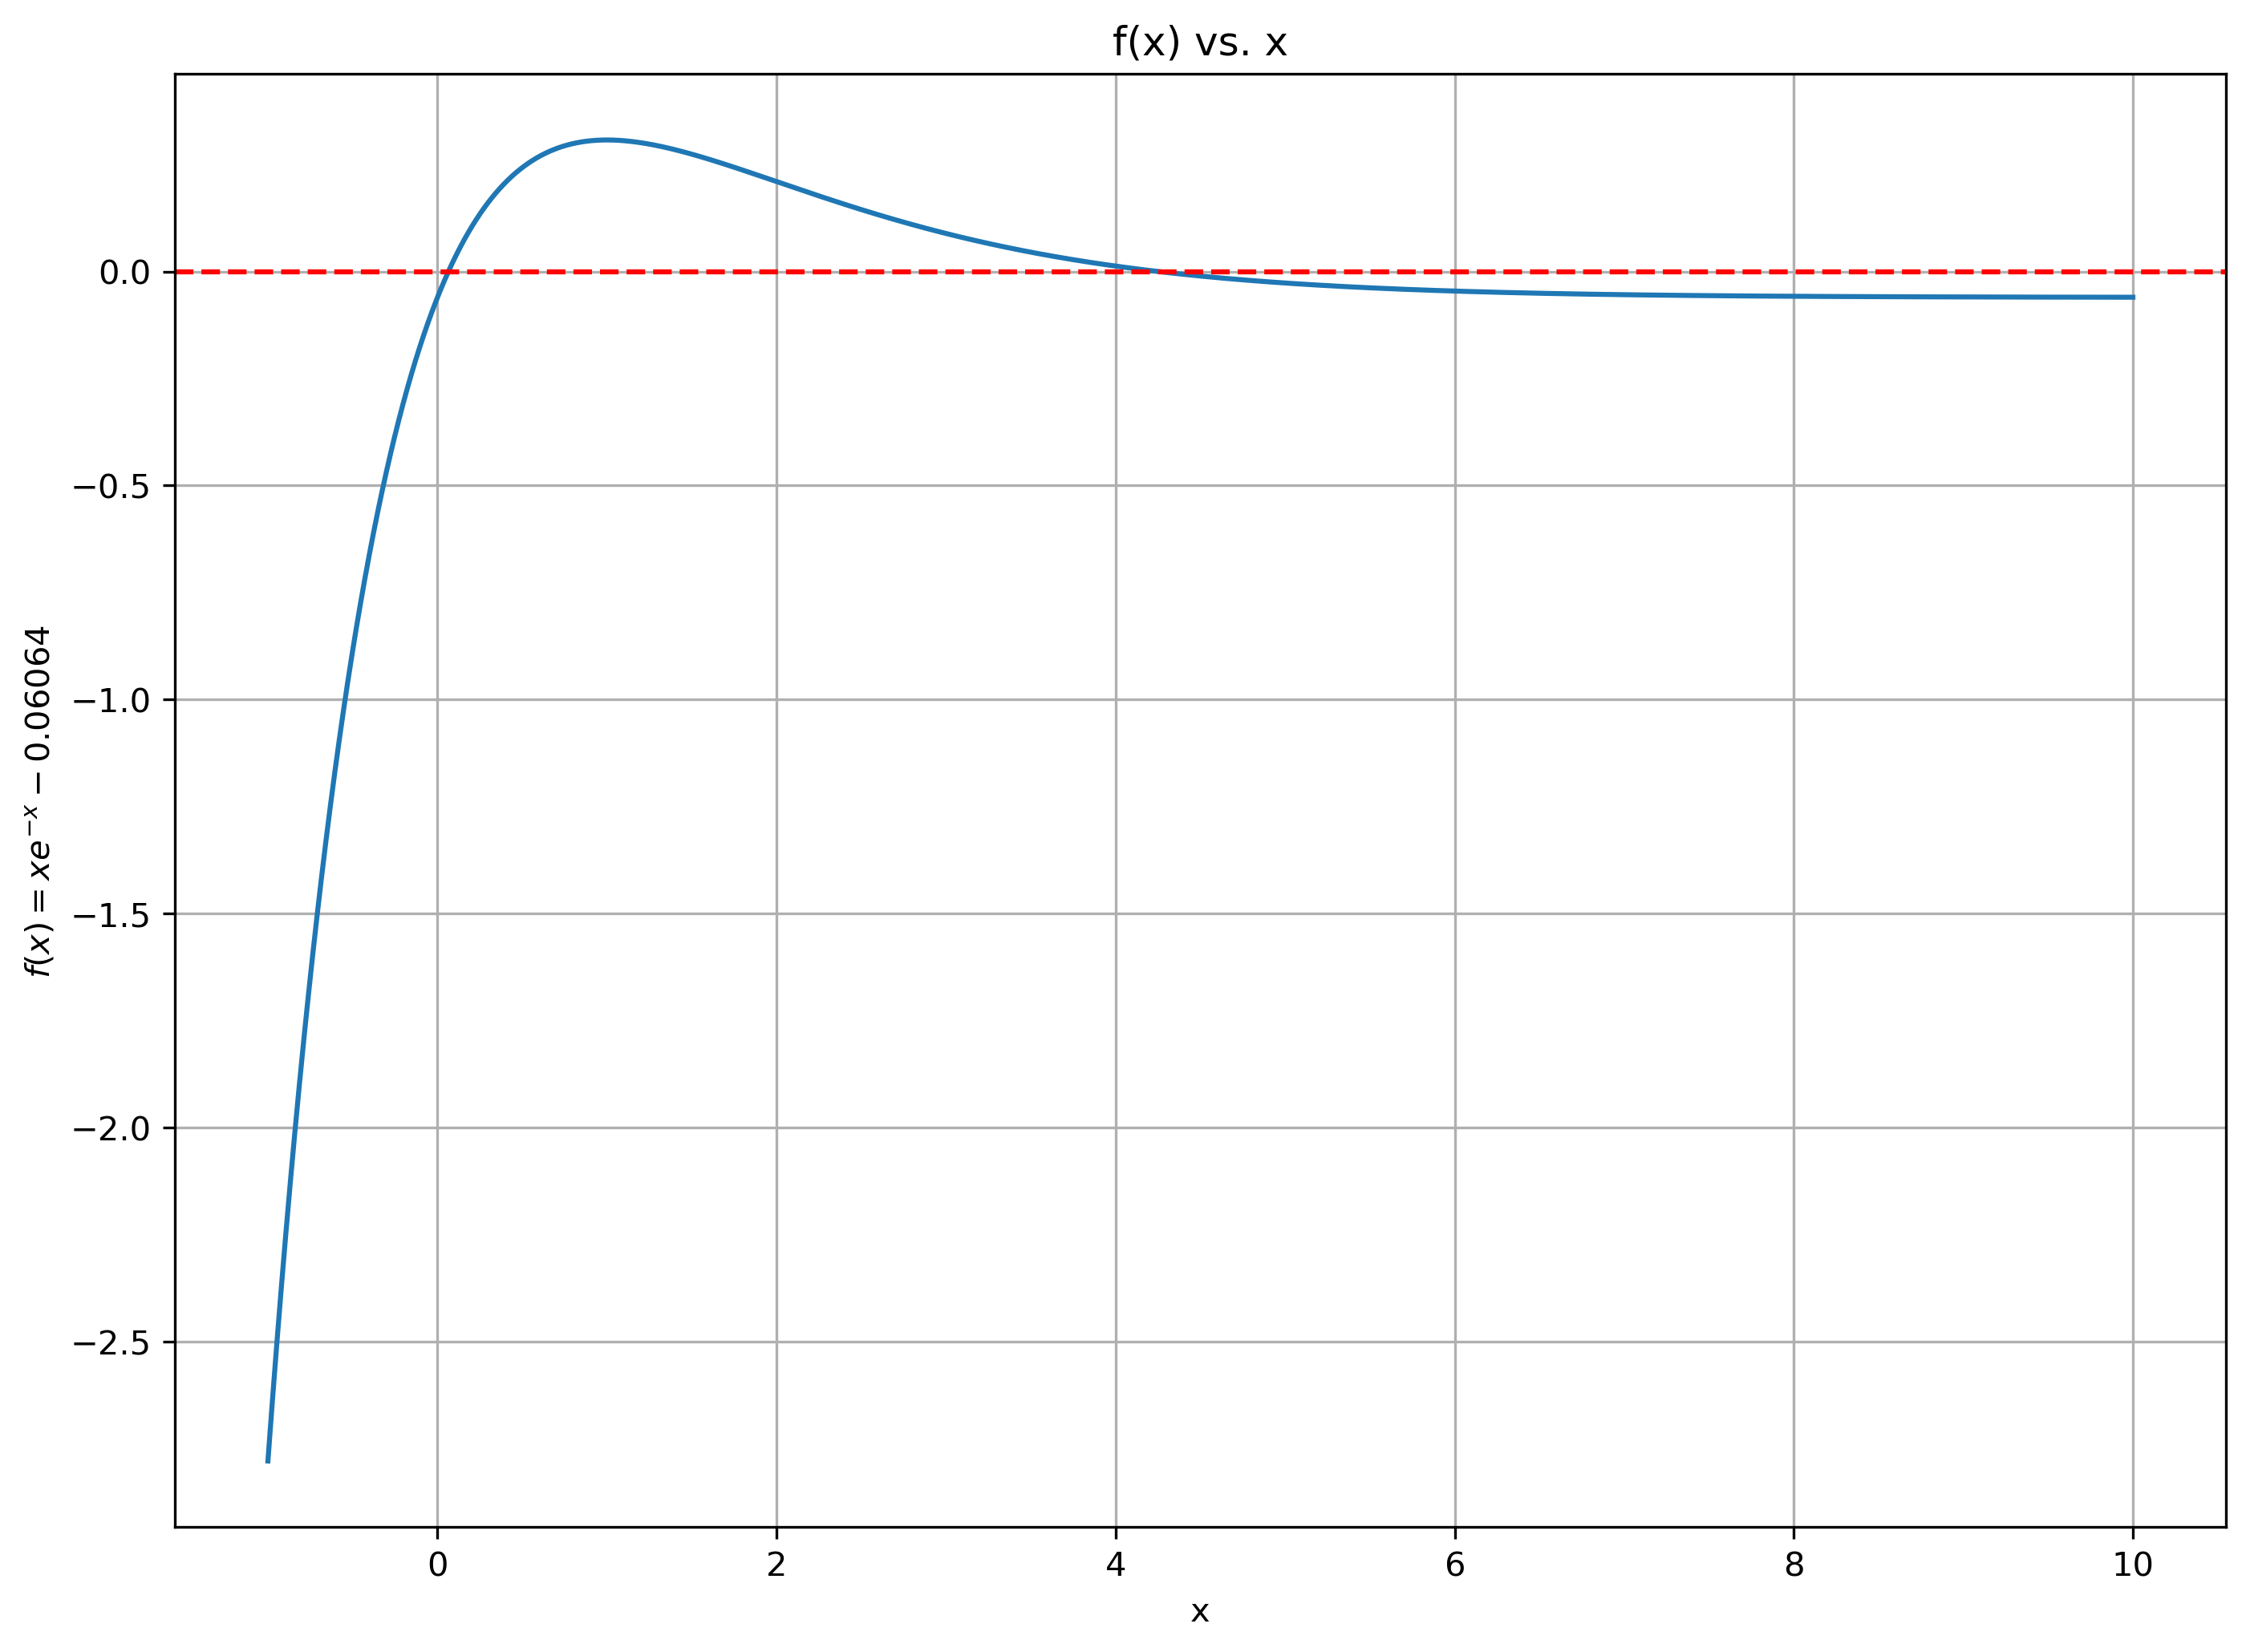
\includegraphics[width=\linewidth]{../figures/f(x)}
	\caption{Graph of f(x) used to verify all the roots that exist.}
	\label{fig:f(x)}
\end{figure}

\begin{figure}[H]
	\centering
	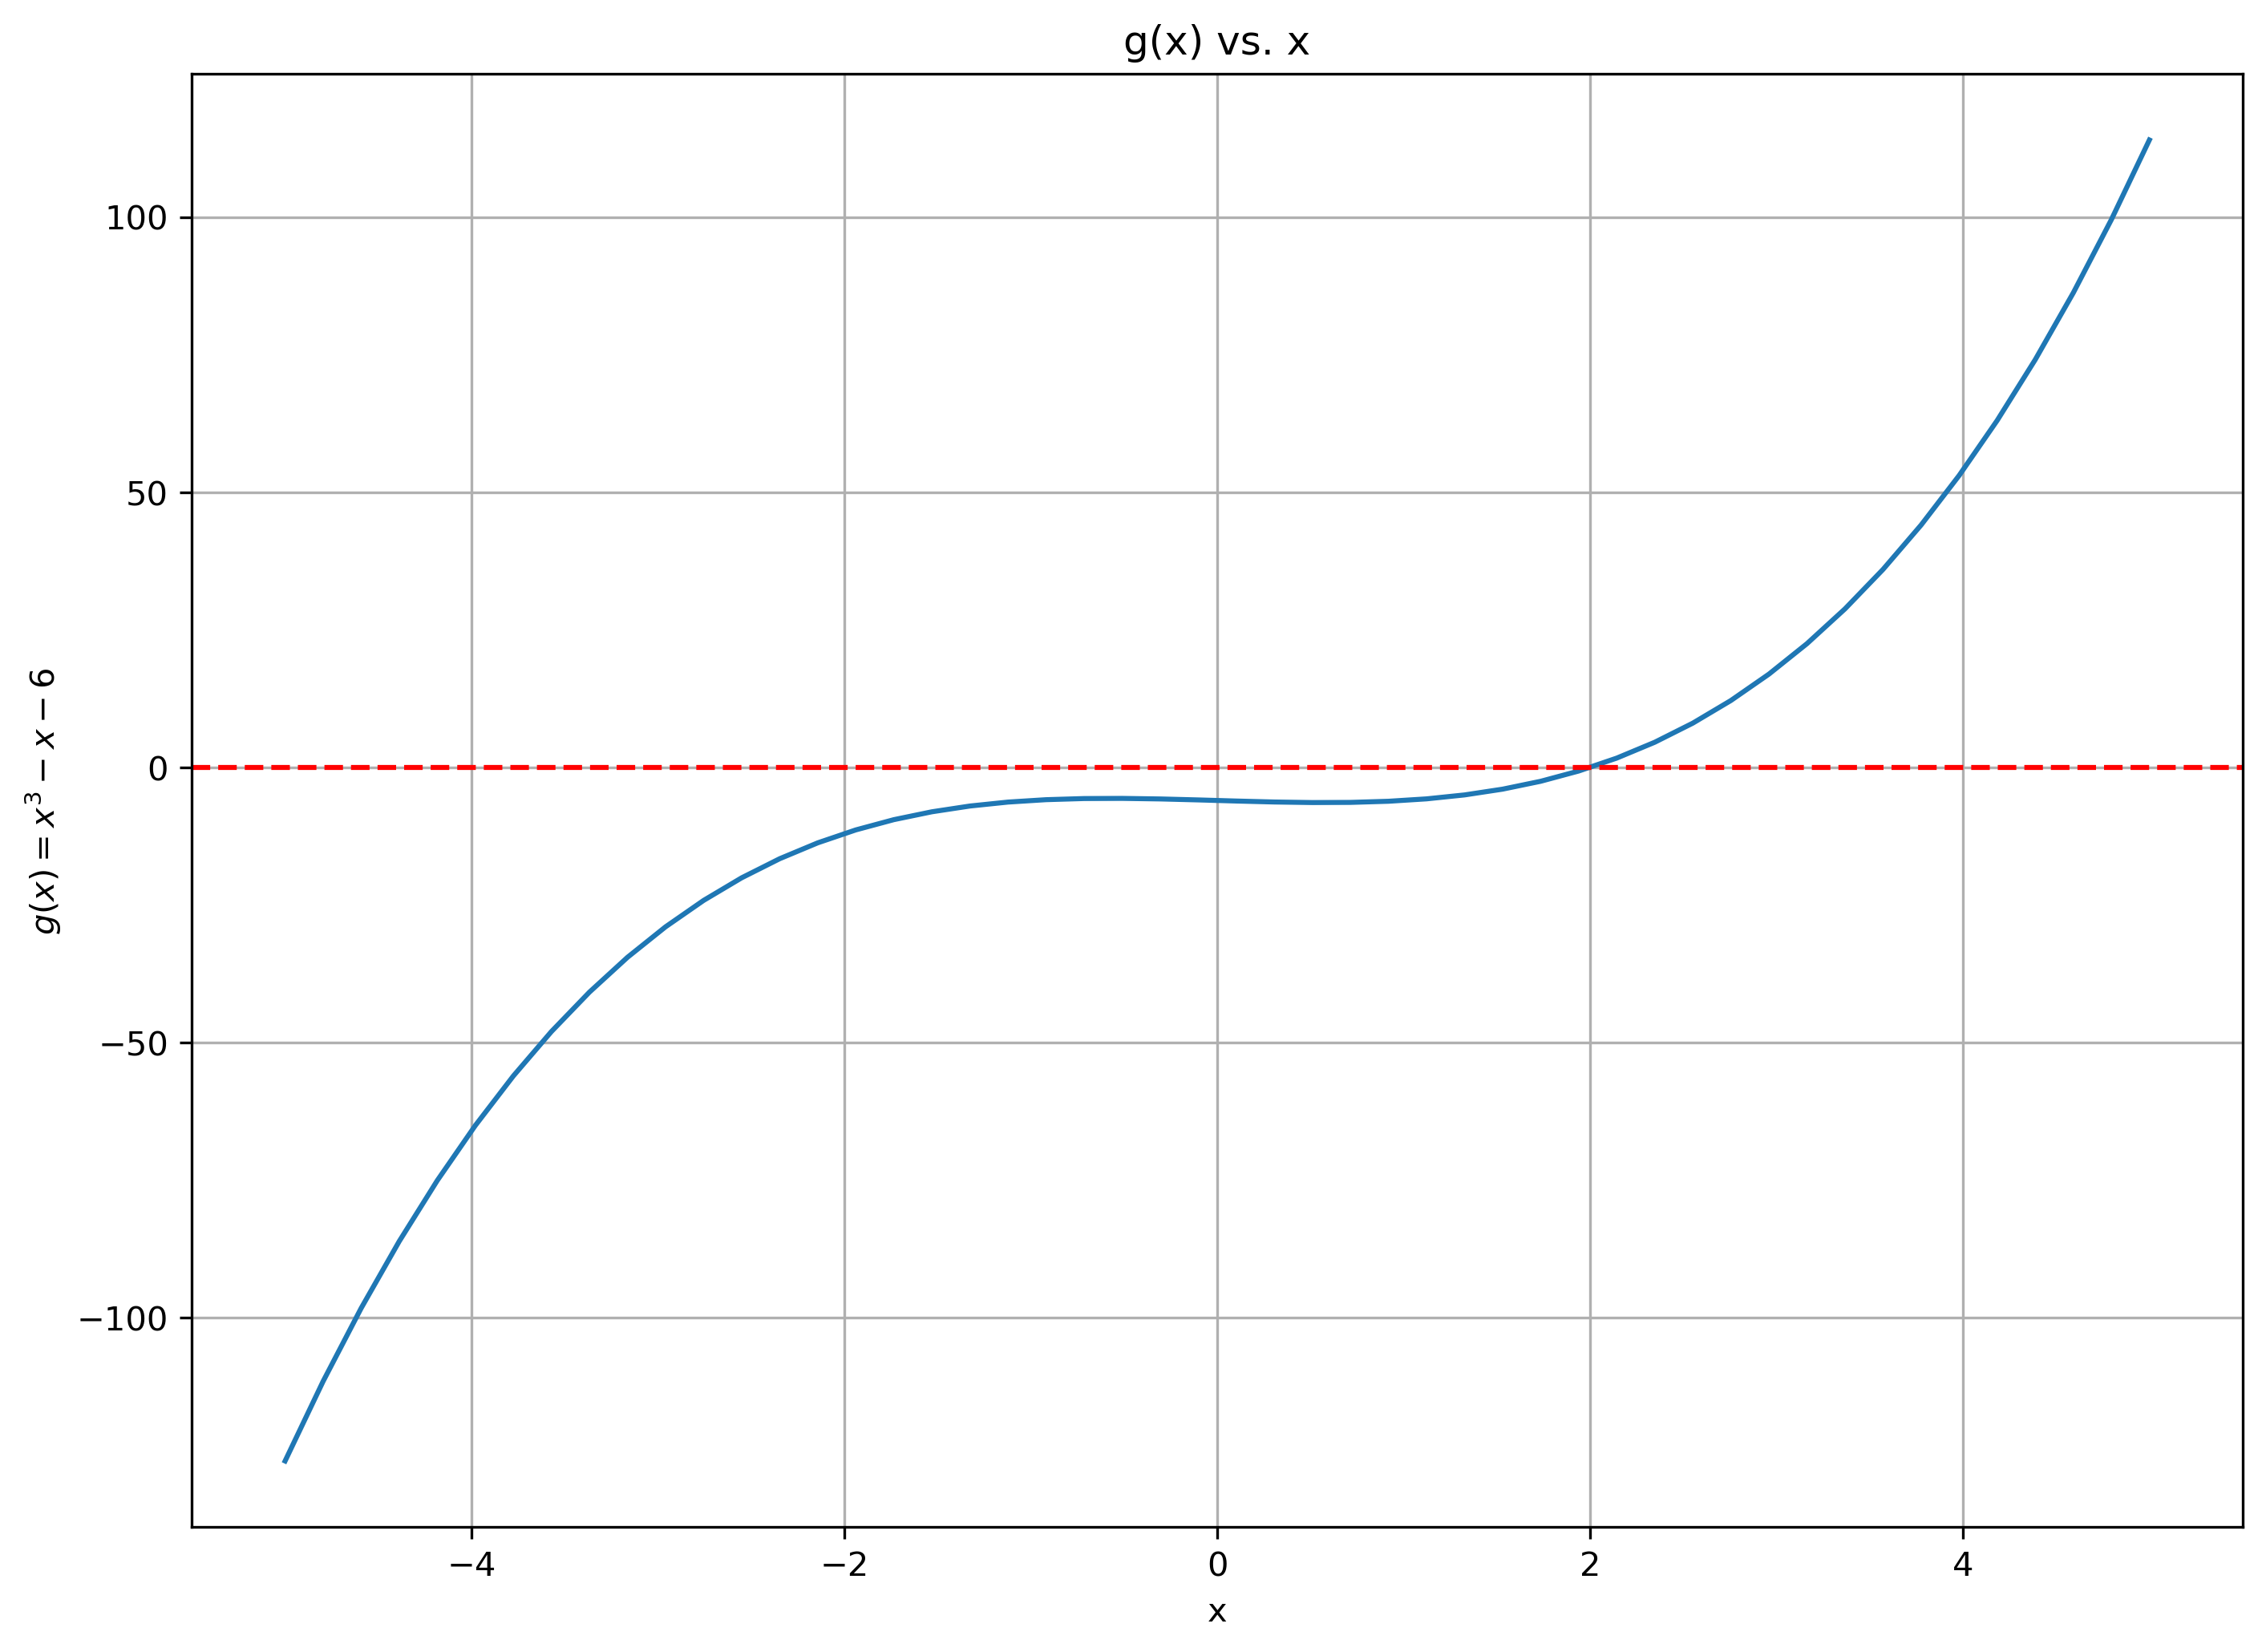
\includegraphics[width=\linewidth]{../figures/g(x)}
	\caption{Graph of g(x) used to verify all the roots that exist.}
	\label{fig:g(x)}
\end{figure}

%%%%%%%%%%%%%%%%%%%%%%%%%%%%%%%%%%%%%%%%%%%%%%%%%%%%%%%%%%%%%%%%%%%%%%%%%%%%%%%%%%%
\subsection{Bisection Plots - f(x):}

\begin{figure}[H]
	\centering
	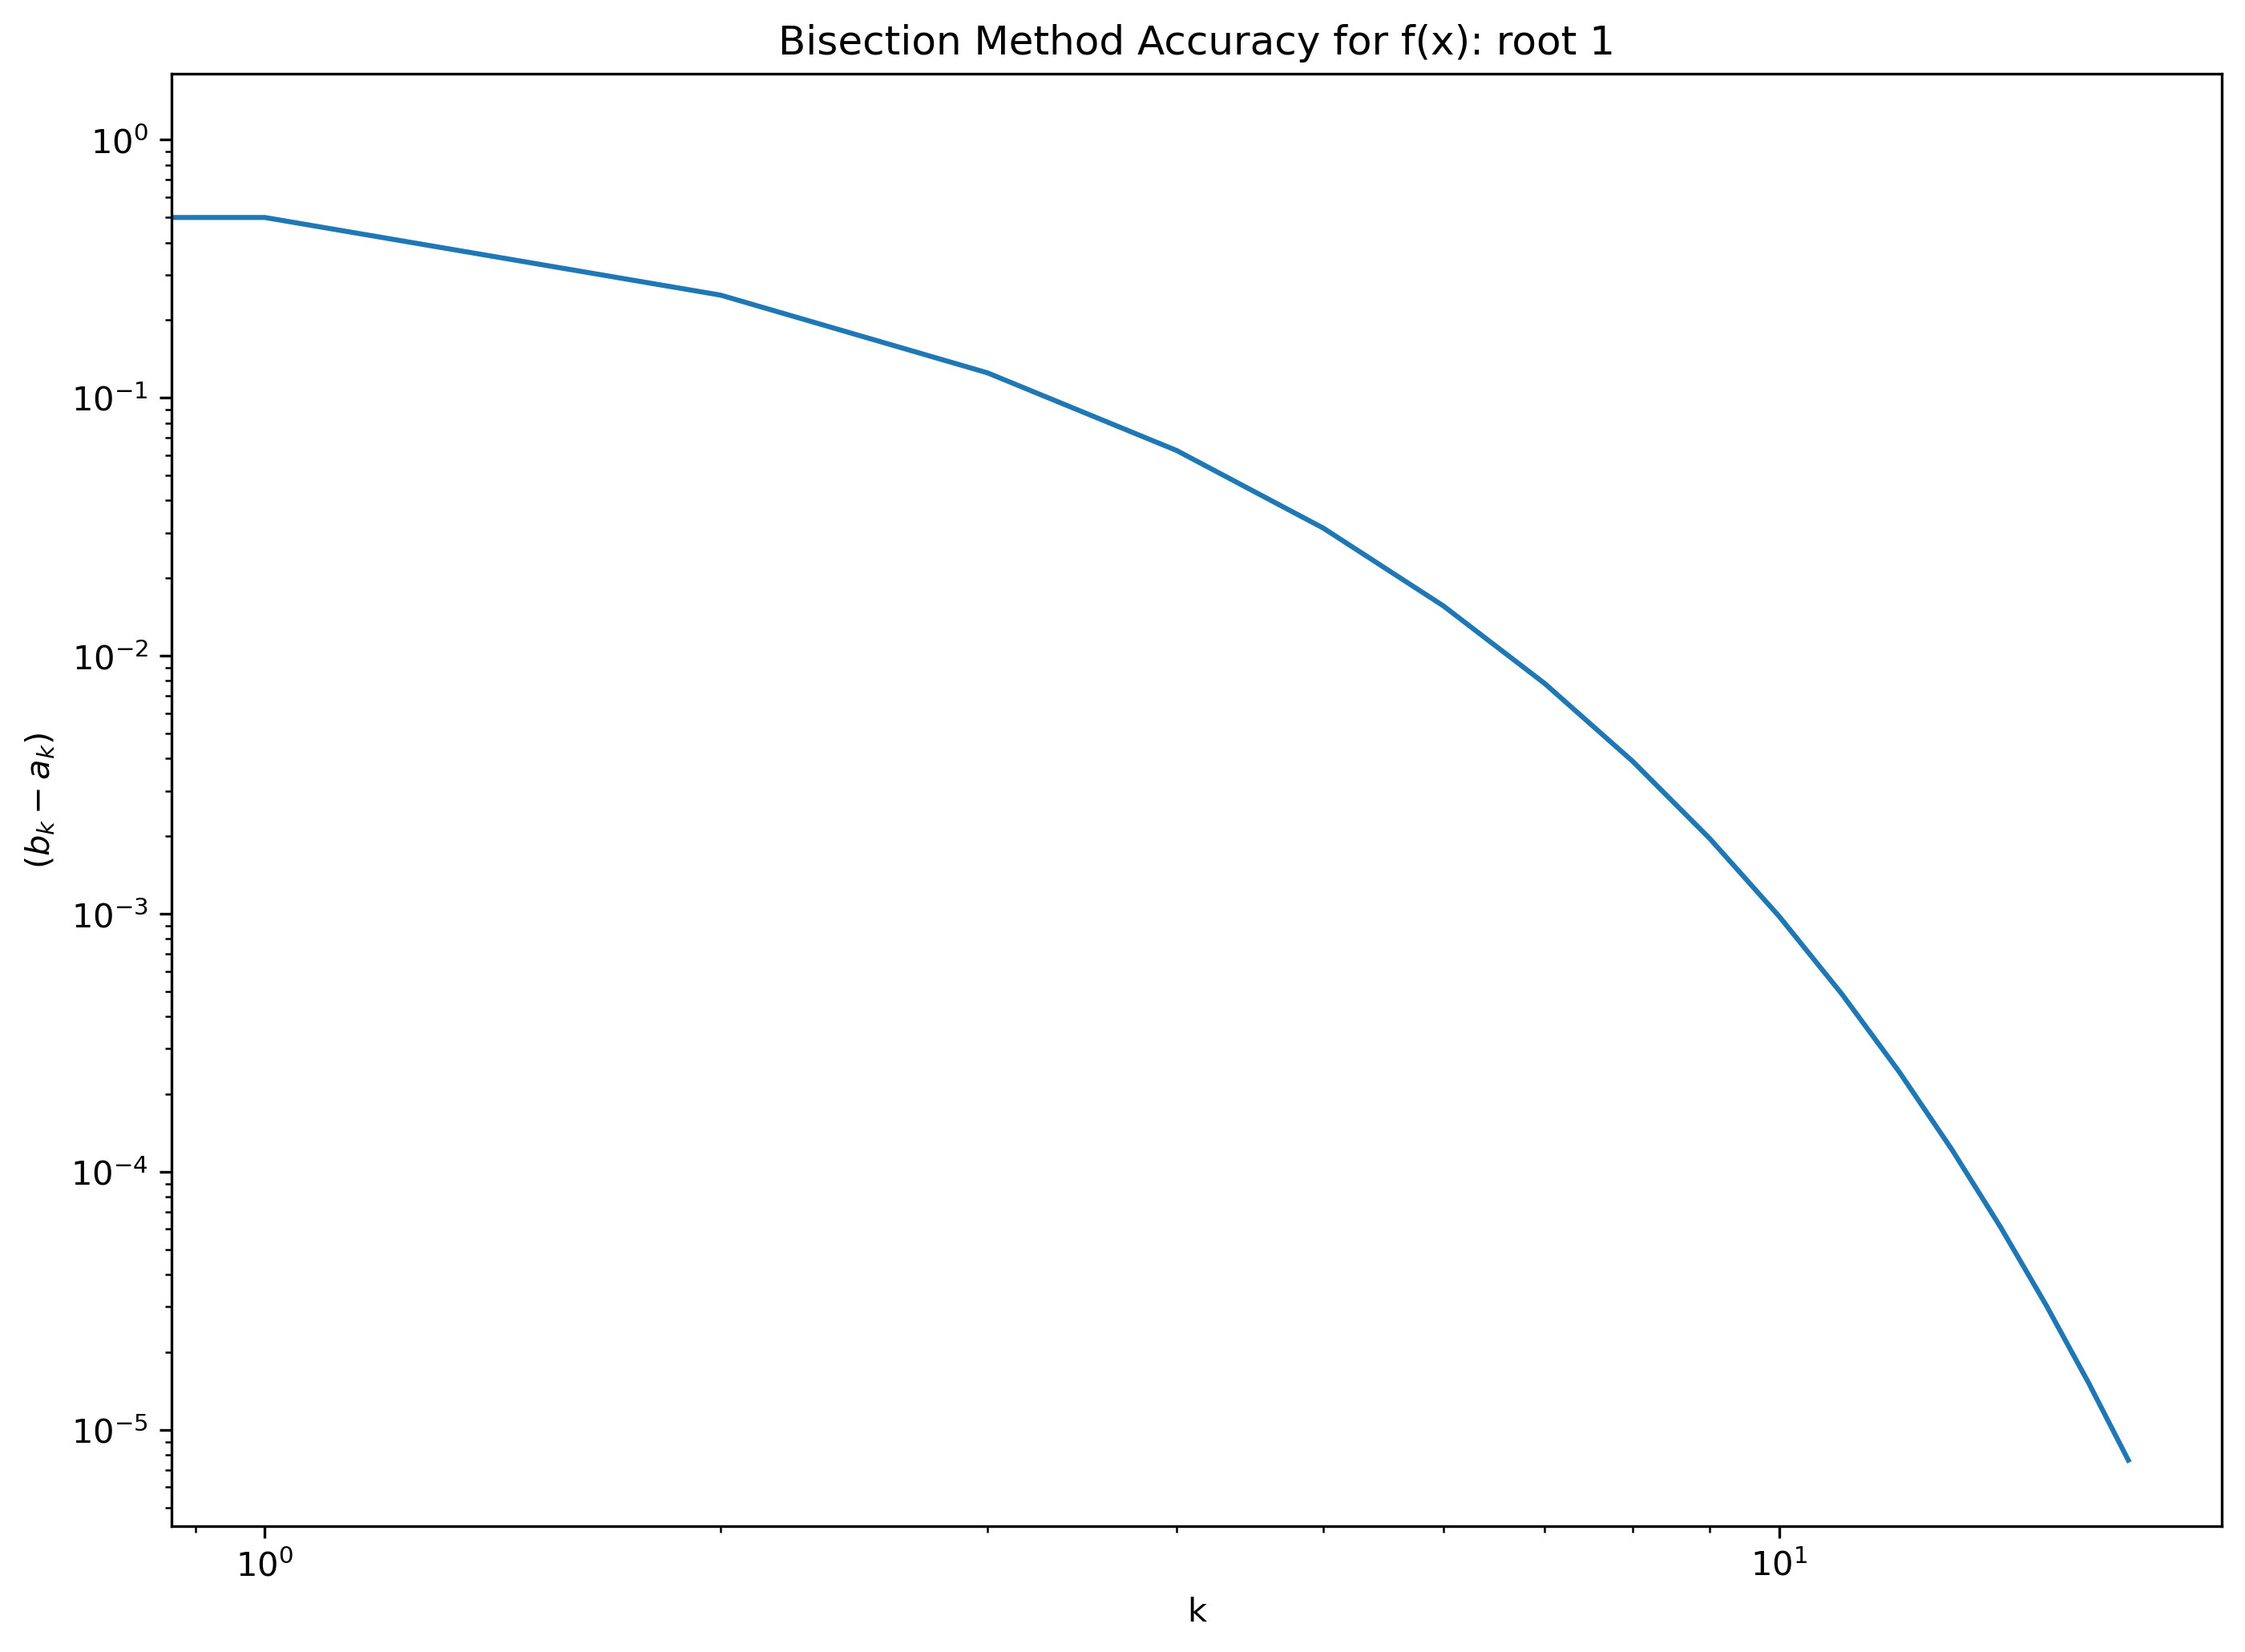
\includegraphics[width=\linewidth]{../figures/Bisection_f_root1}
	\caption{Interval size per iteration step for the first root of $f(x) = xe^{-x} - 0.06064$ using the bisection method, shown in logscale.}
	\label{fig:bisec_f1}
\end{figure}

\begin{figure}[H]
	\centering
	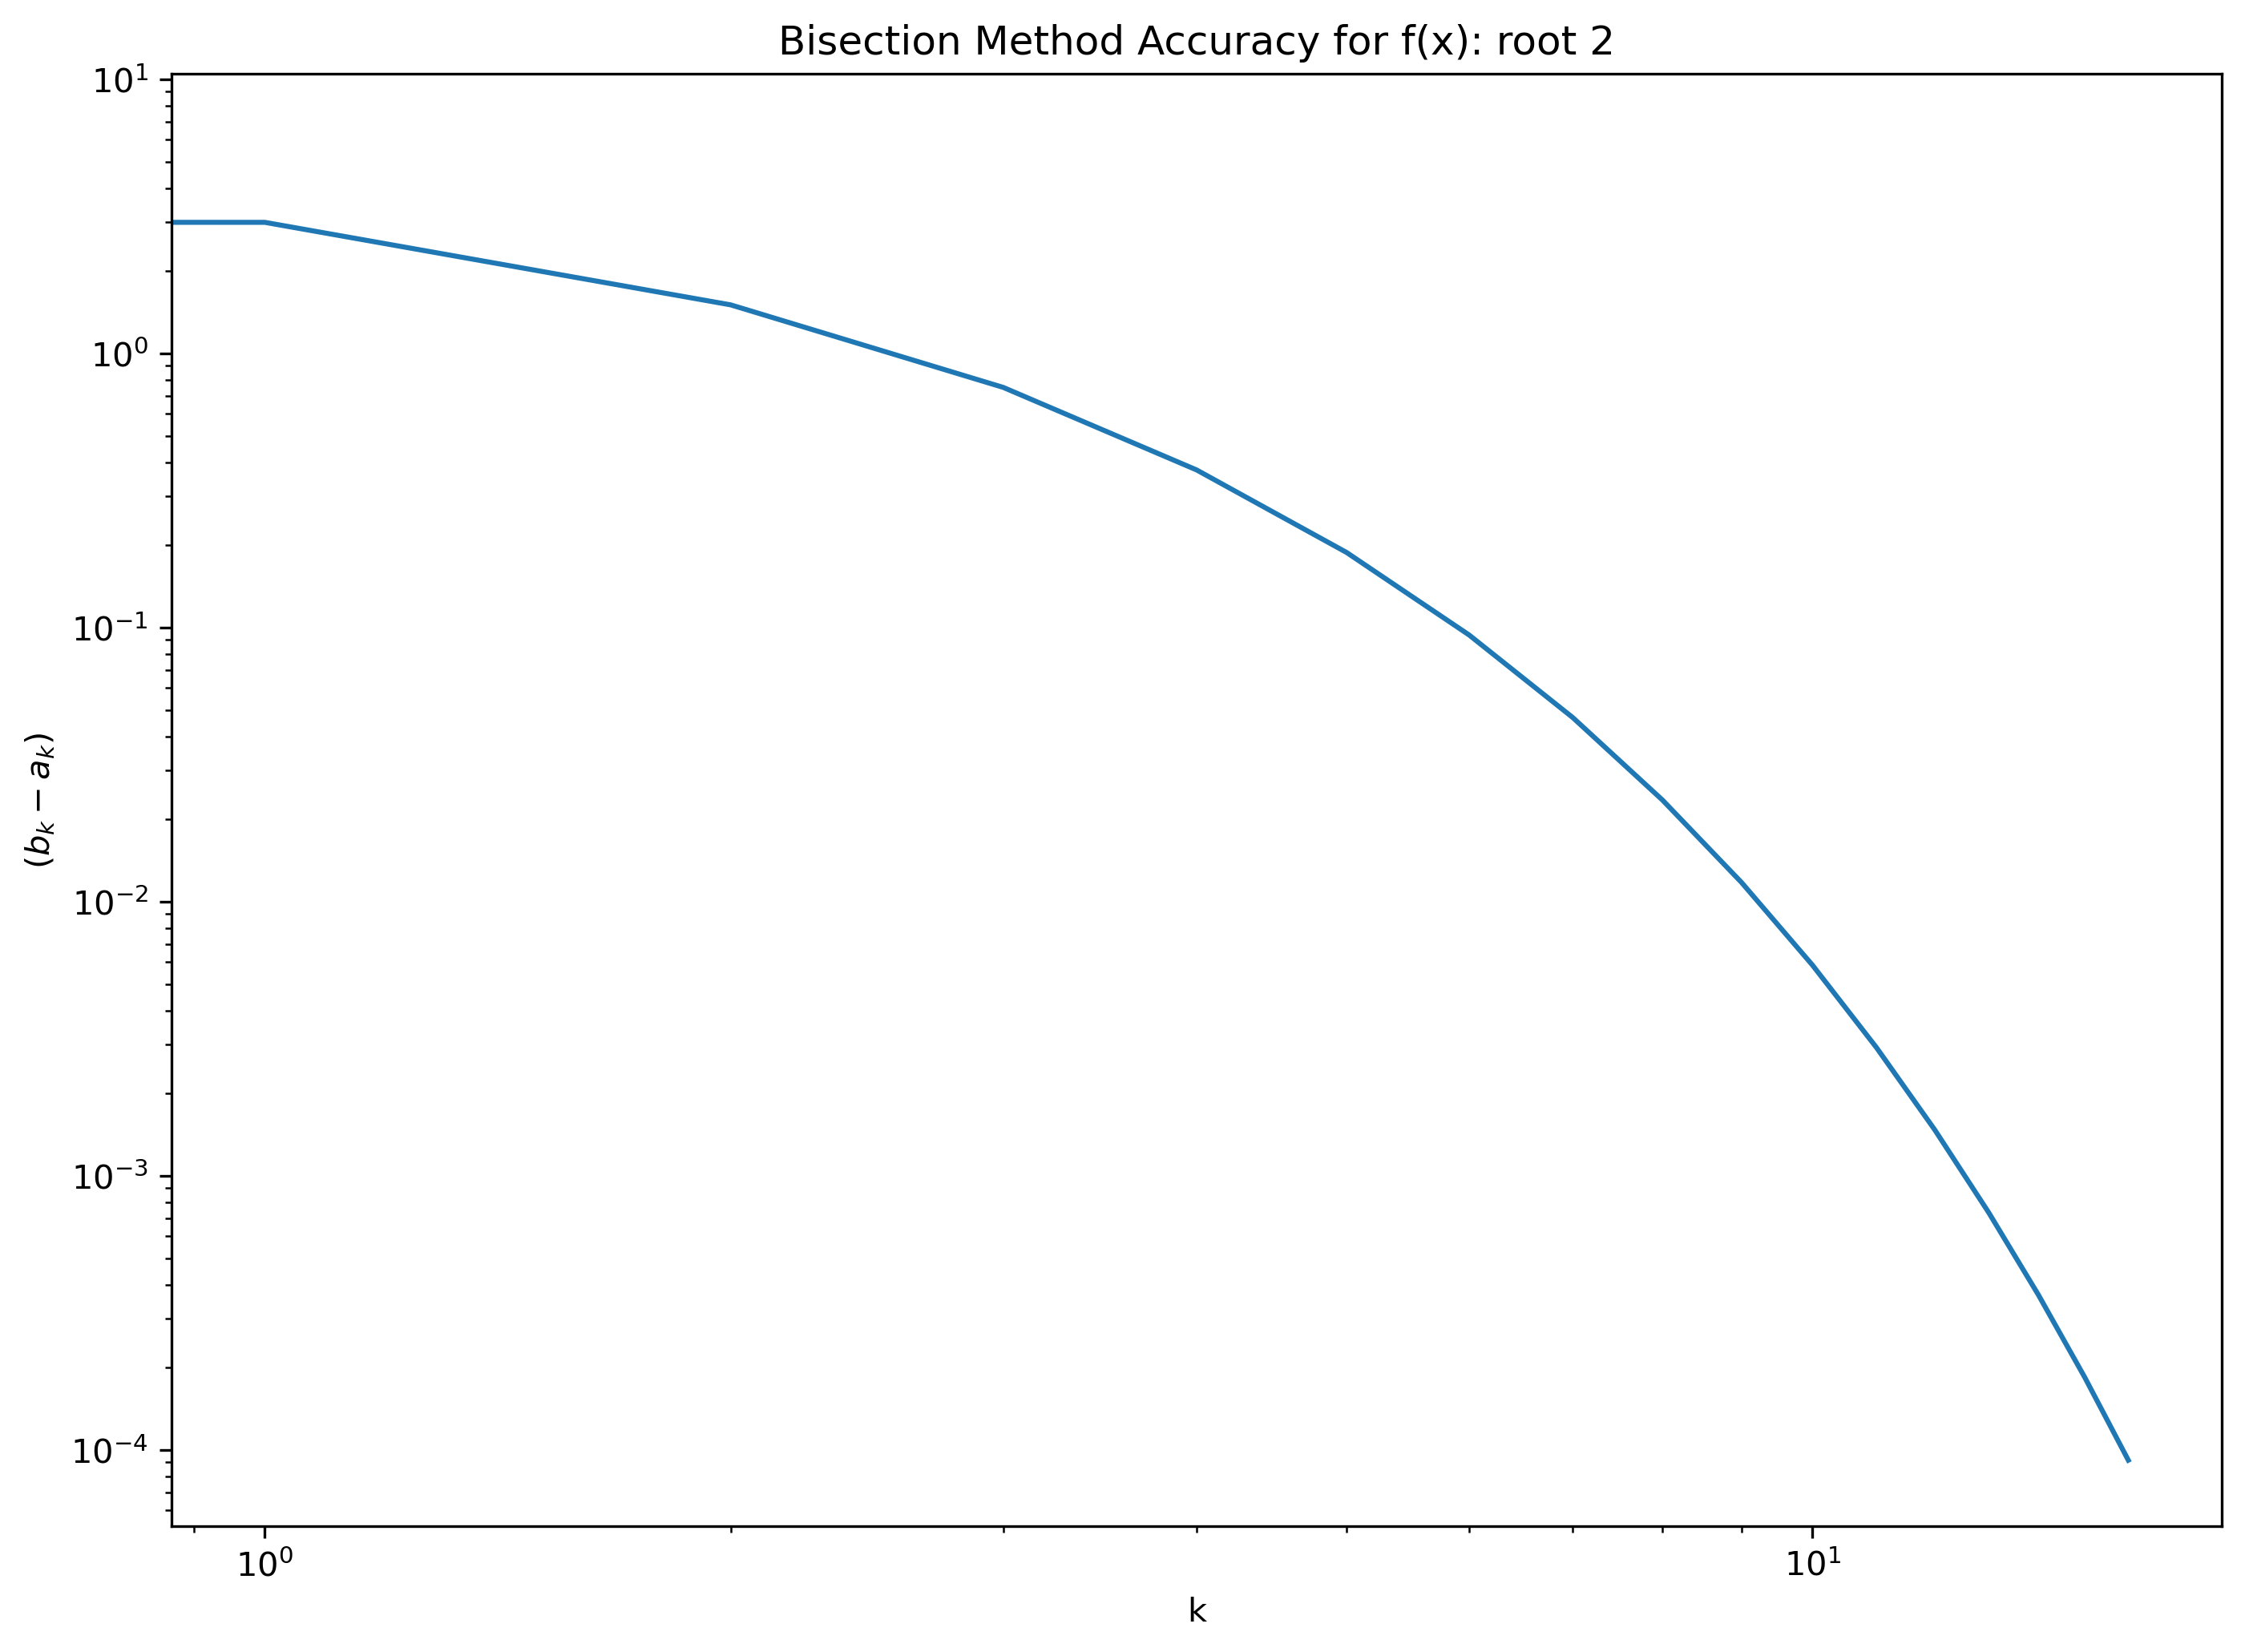
\includegraphics[width=\linewidth]{../figures/Bisection_f_root2}
	\caption{Interval size per iteration step for the second root of $f(x) = xe^{-x} - 0.06064$ using the bisection method, shown in logscale.}
	\label{fig:bisec_f2}
\end{figure}

%%%%%%%%%%%%%%%%%%%%%%%%%%%%%%%%%%%%%%%%%%%%%%%%%%%%%%%%%%%%%%%%%%%%%%%%%%%%%%%%%%%
\subsection{Newton's Method Plots - f(x):}
\begin{figure}[H]
	\centering
	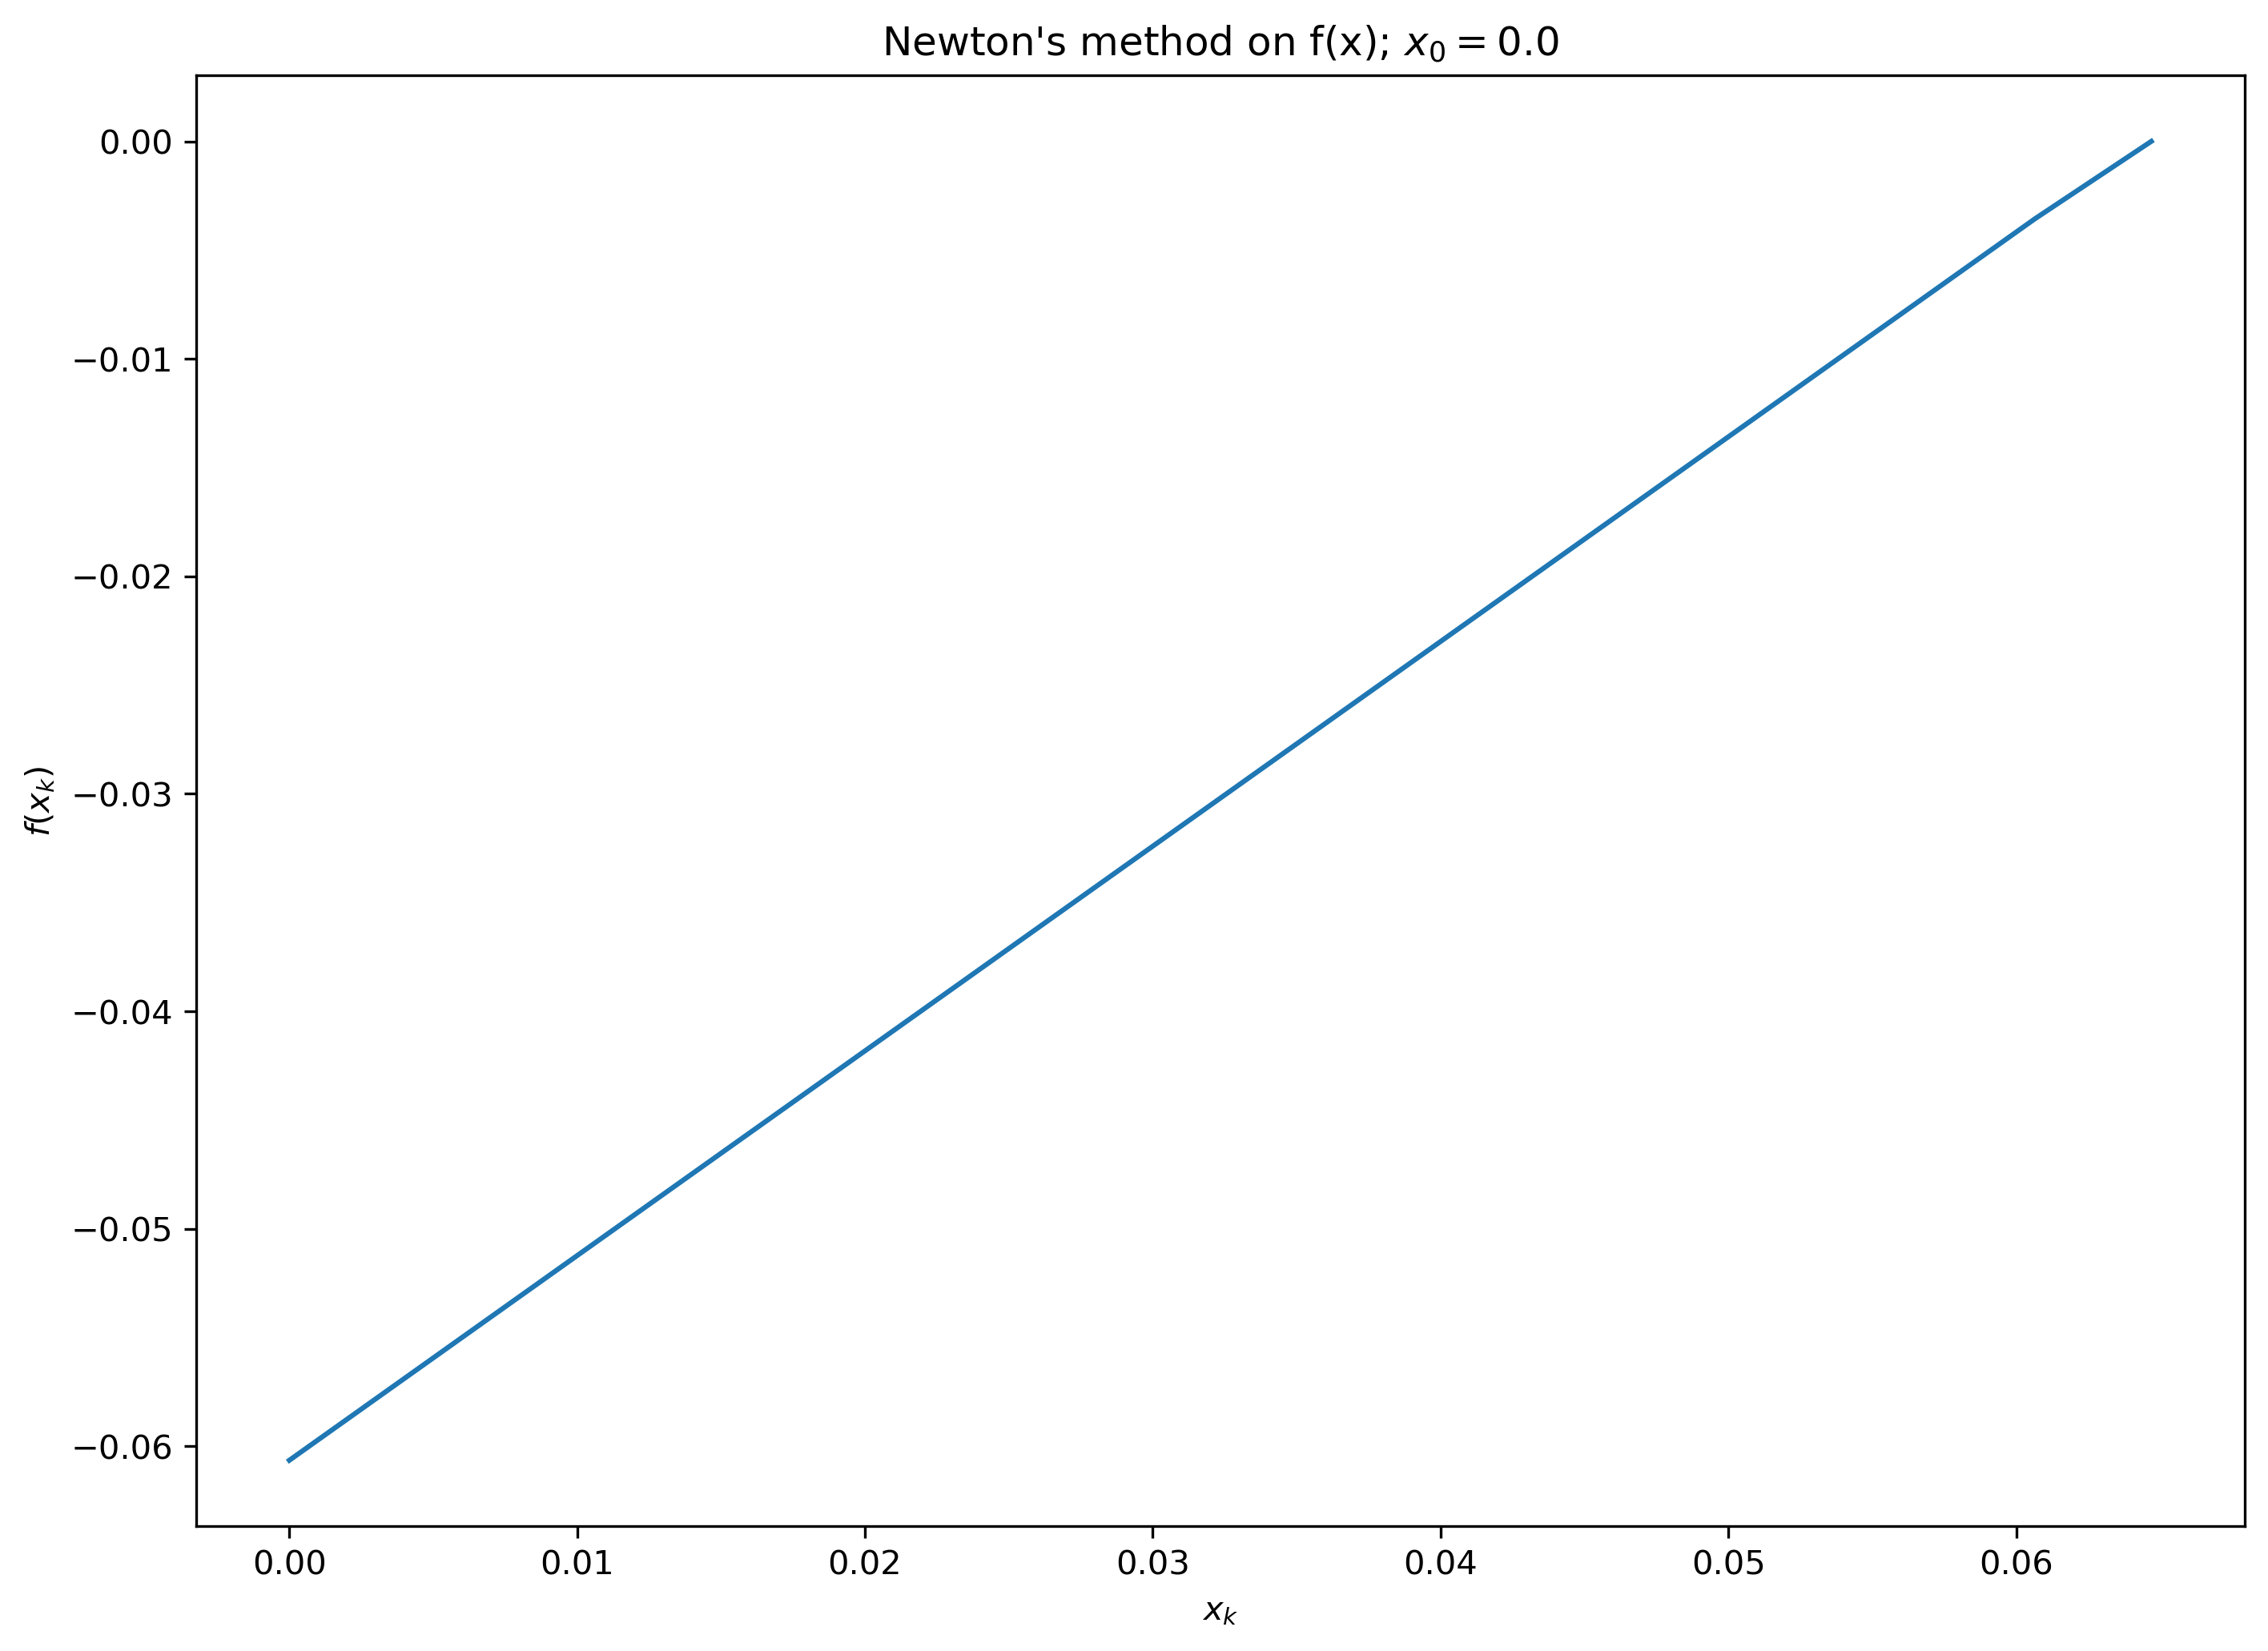
\includegraphics[width=\linewidth]{../figures/Newtons_f_0.0}
	\caption{Function values, $f(x_k)$, versus $x_k$ for each $k$ using Newton's method with $x_0 = 0.0$.}
	\label{fig:newton_f_0.0}
\end{figure}

\begin{figure}[H]
	\centering
	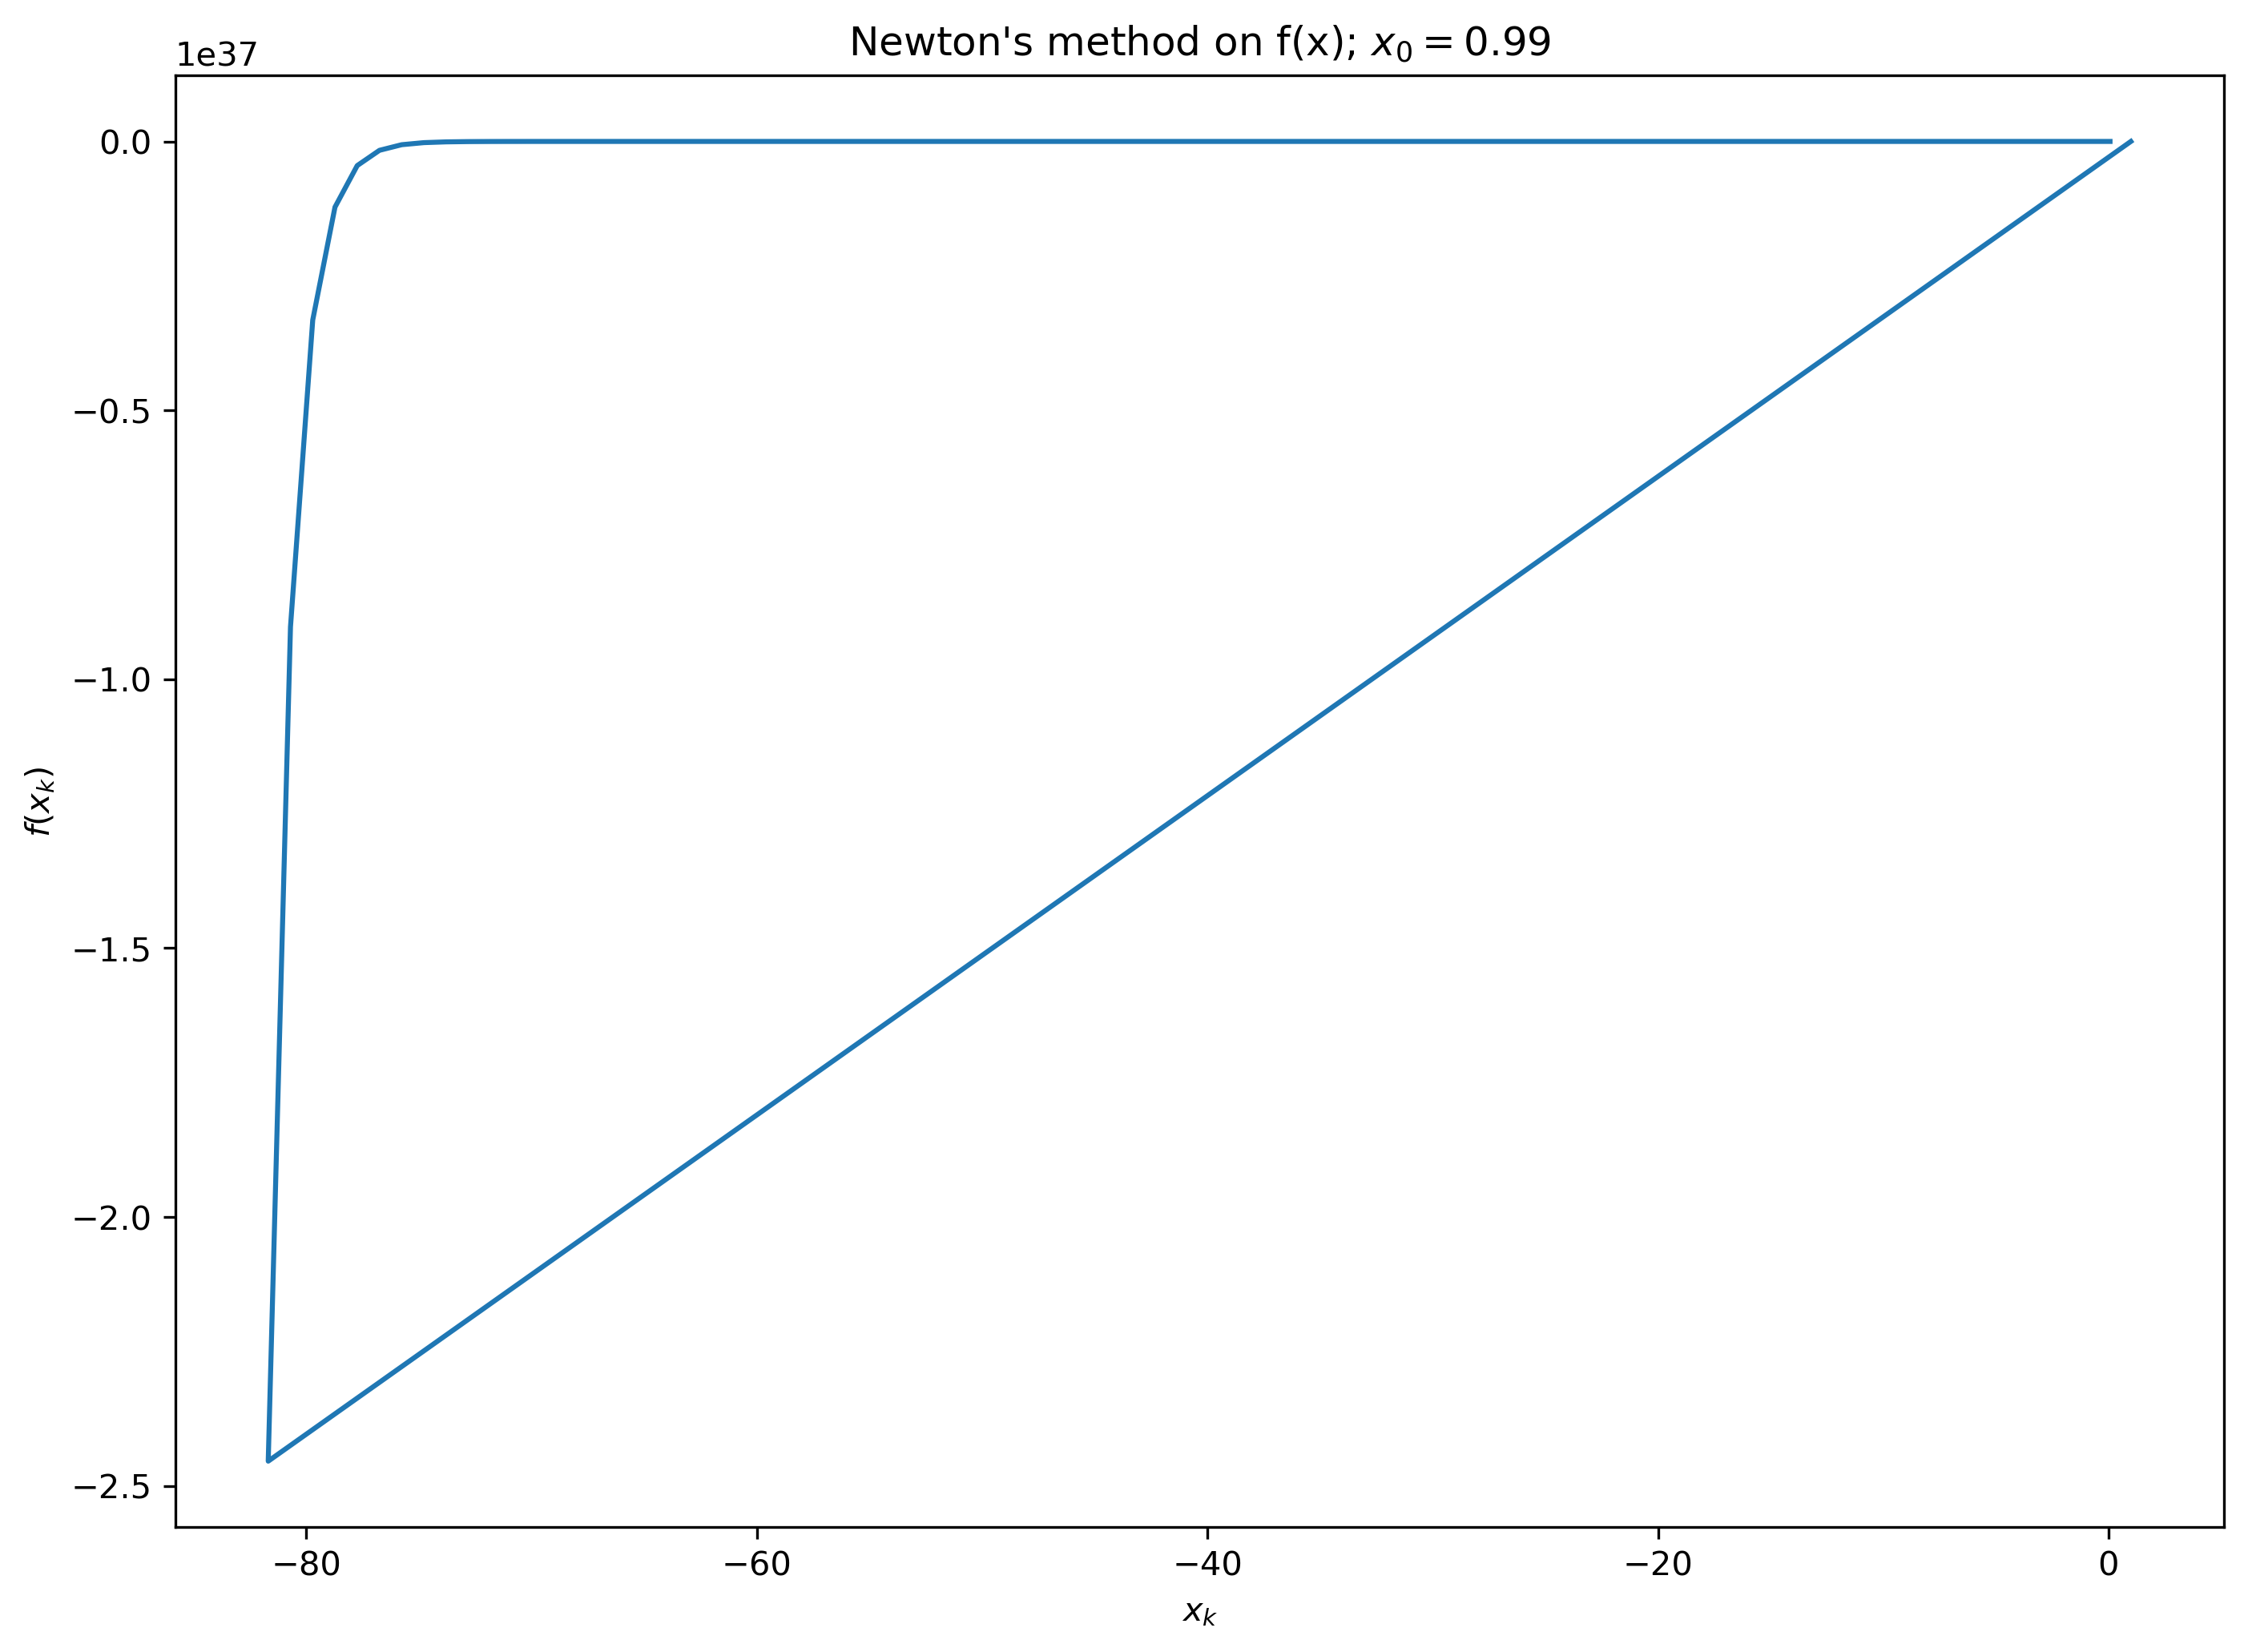
\includegraphics[width=\linewidth]{../figures/Newtons_f_0.99}
	\caption{Function values, $f(x_k)$, versus $x_k$ for each $k$ using Newton's method with $x_0 = 0.99$.}
	\label{fig:newton_f_0.99}
\end{figure}

\begin{figure}[H]
	\centering
	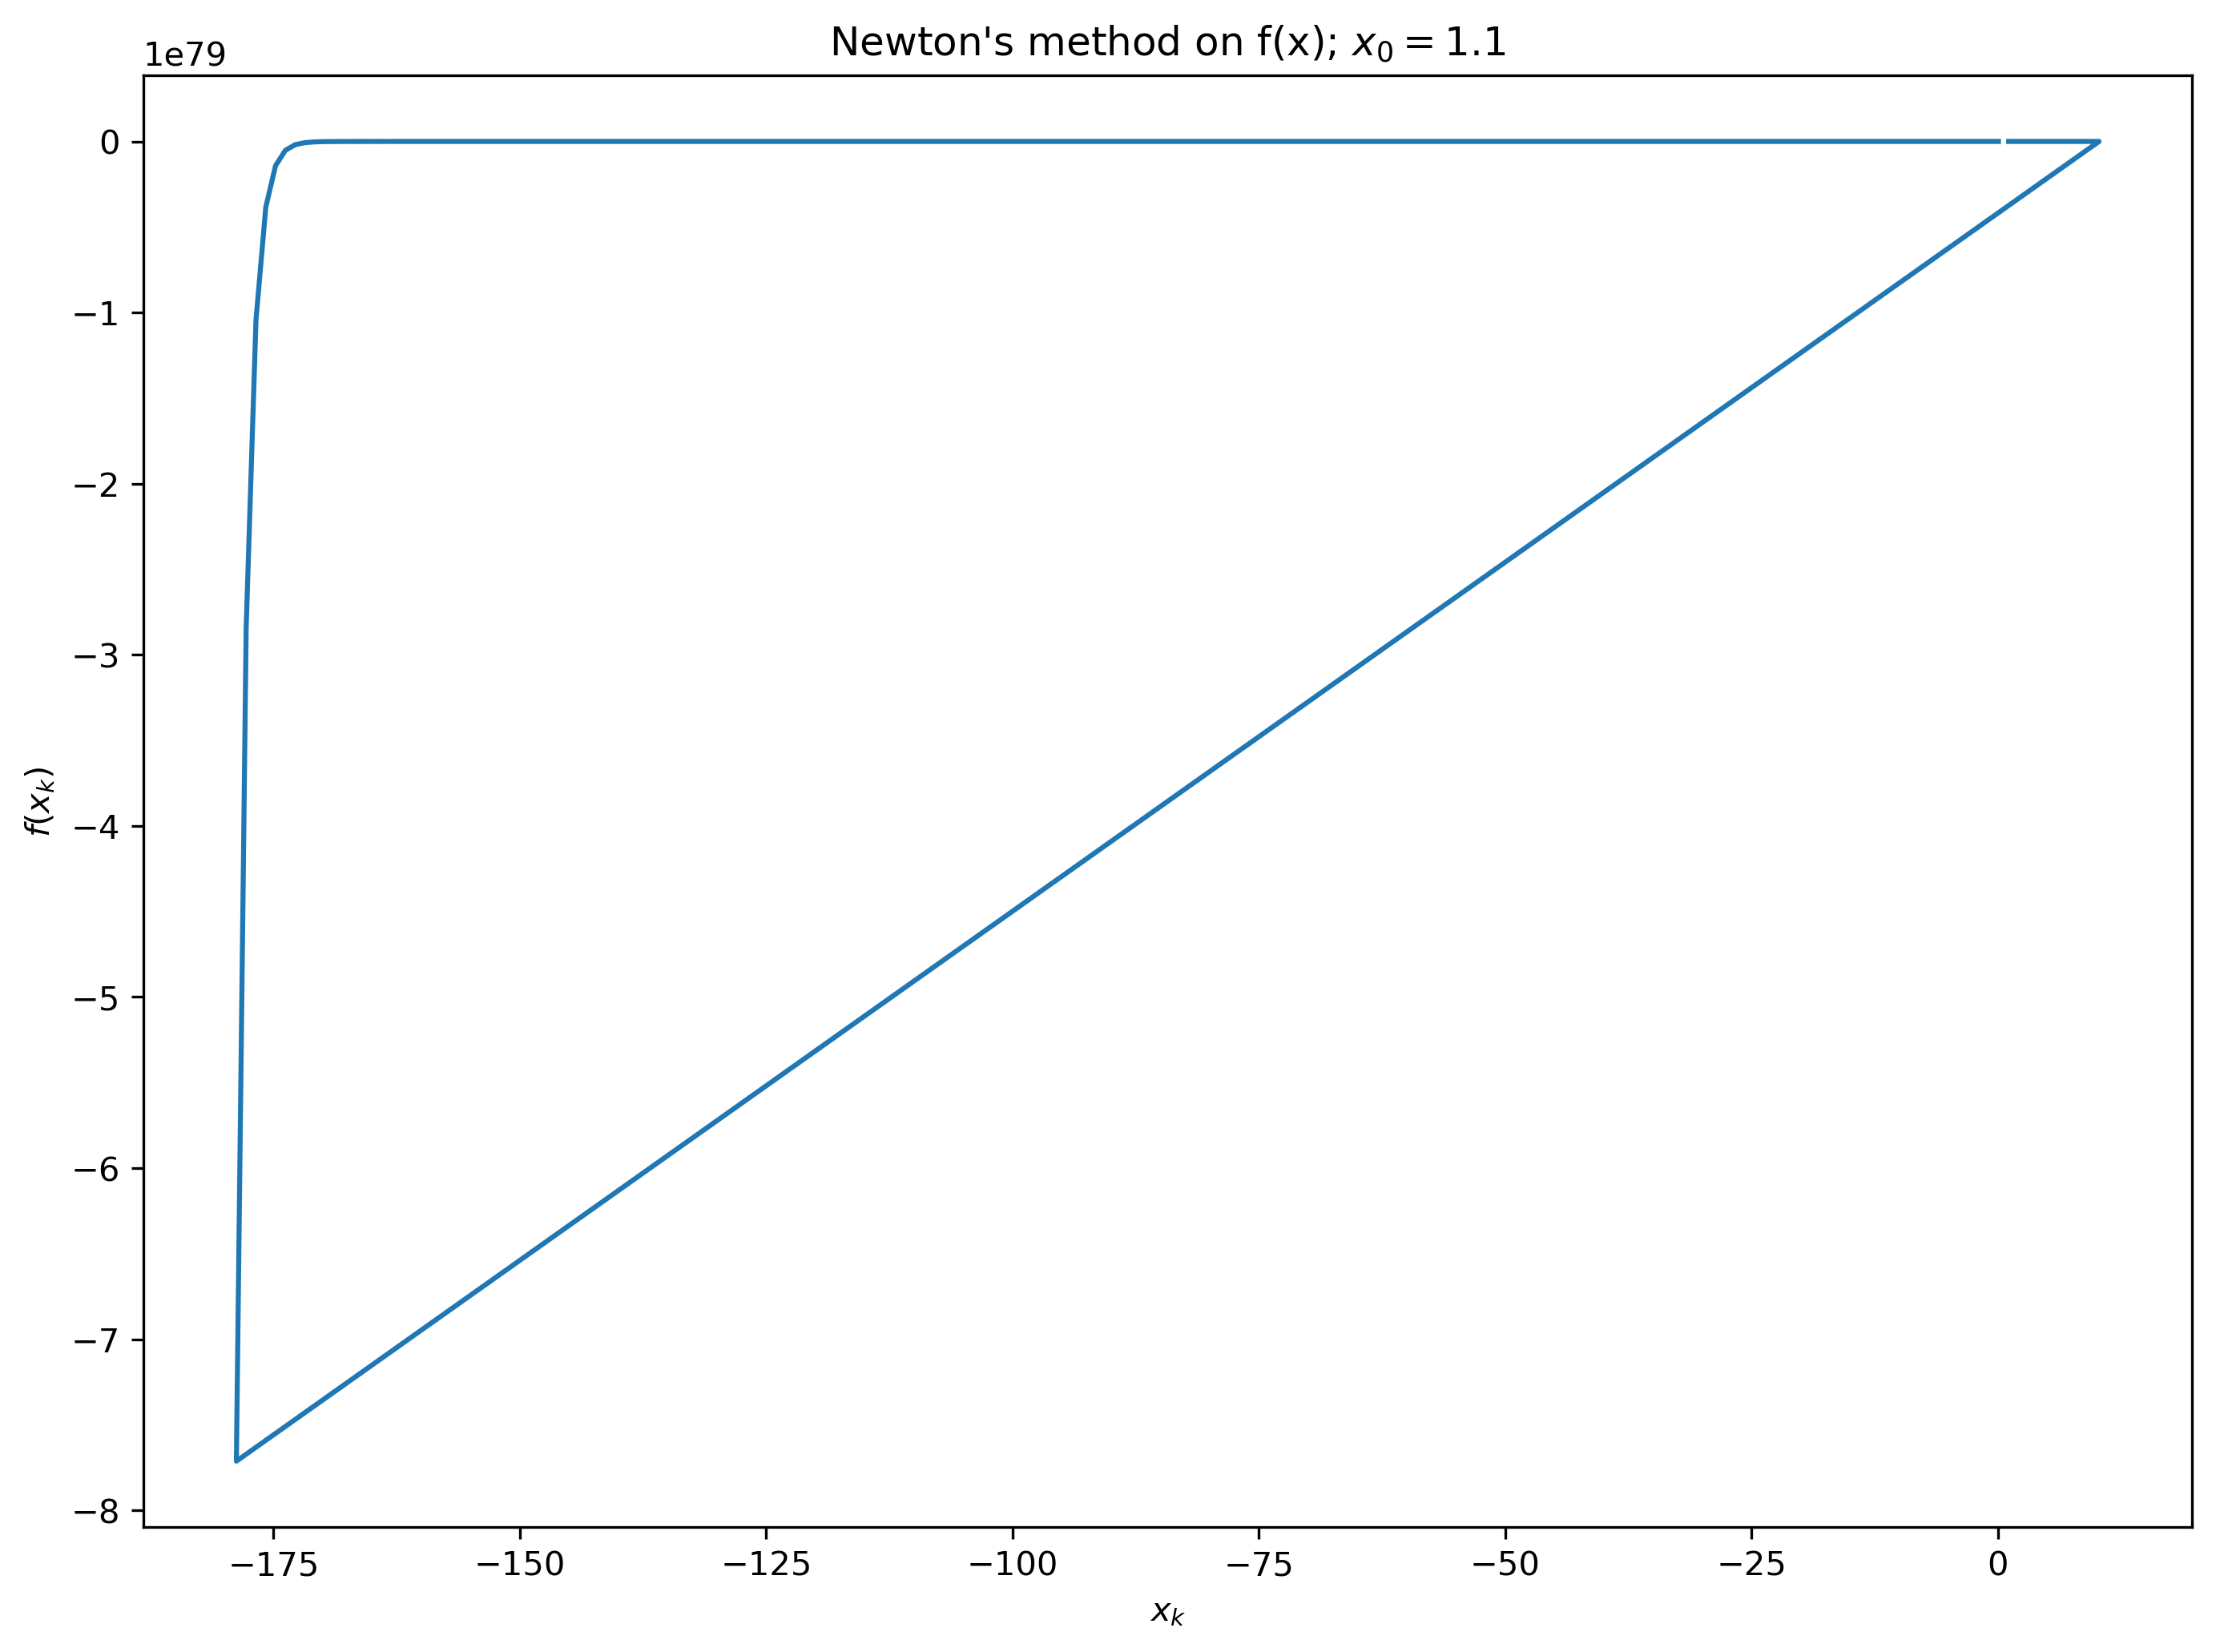
\includegraphics[width=\linewidth]{../figures/Newtons_f_1.1}
	\caption{Function values, $f(x_k)$, versus $x_k$ for each $k$ using Newton's method with $x_0 = 1.1$.}
	\label{fig:newton_f_1.1}
\end{figure}

\begin{figure}[H]
	\centering
	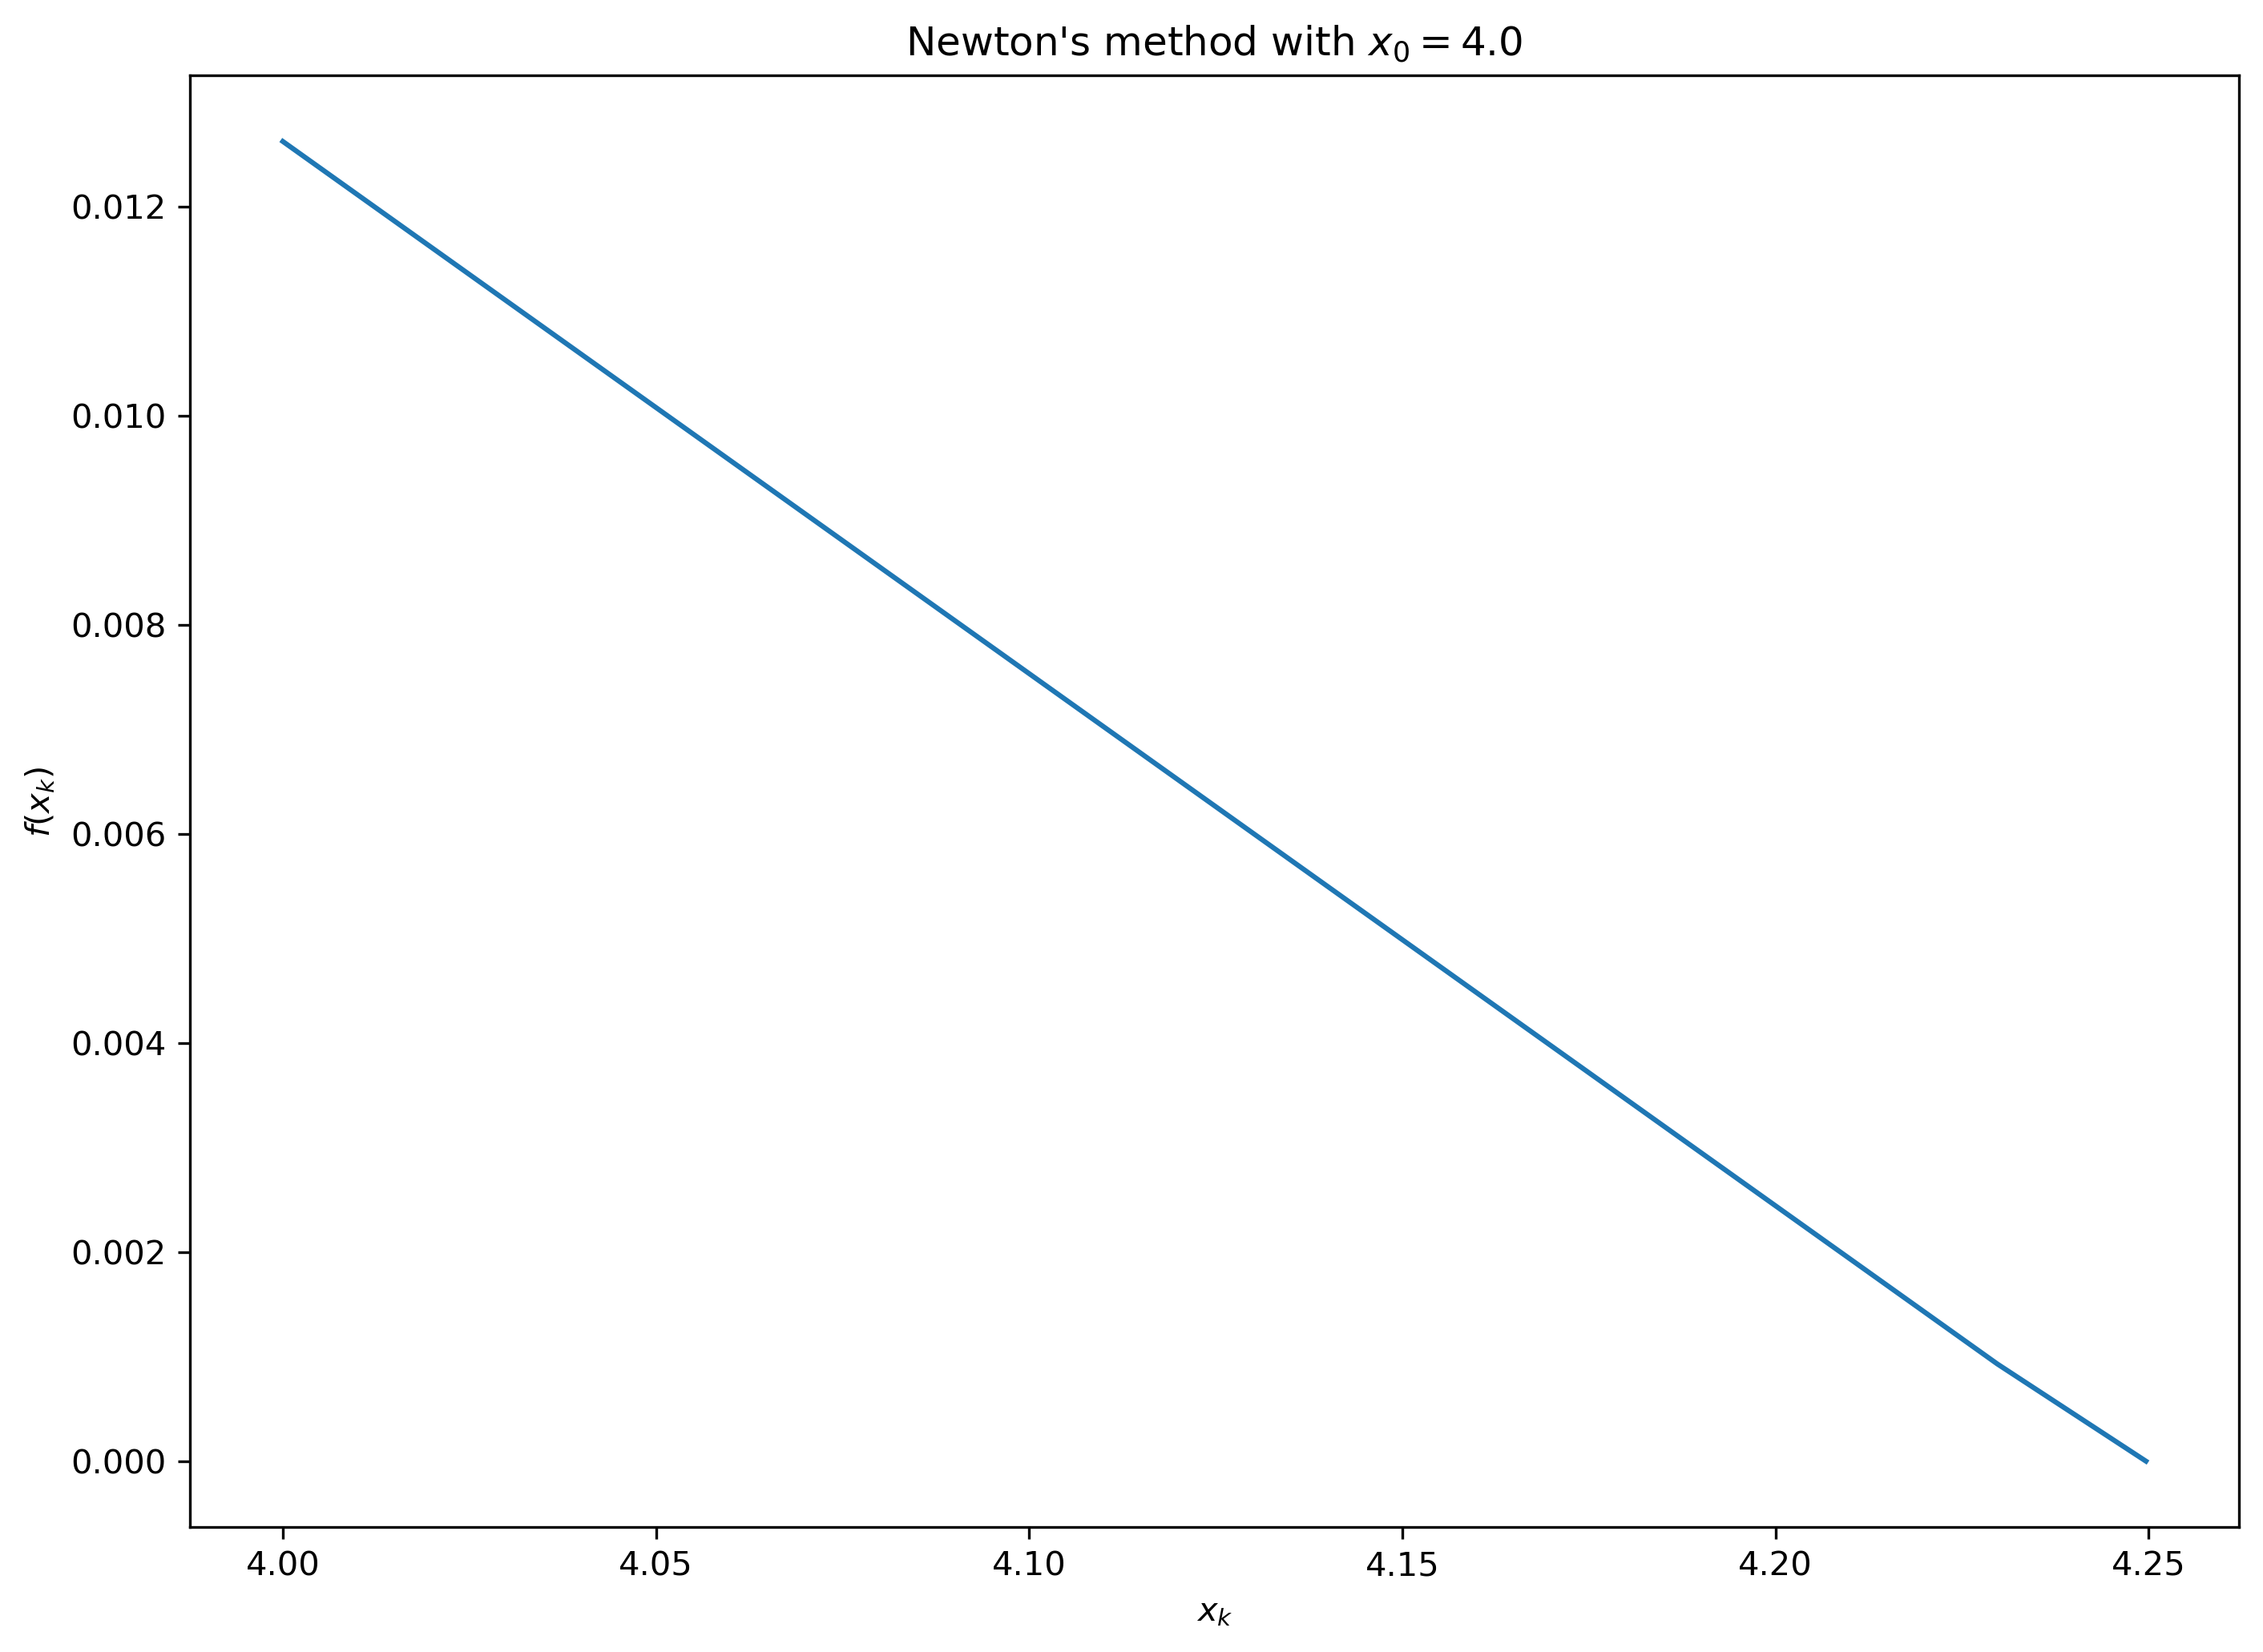
\includegraphics[width=\linewidth]{../figures/Newtons_f_4.0}
	\caption{Function values, $f(x_k)$, versus $x_k$ for each $k$ using Newton's method with $x_0 = 4.0$.}
	\label{fig:newton_f_4.0}
\end{figure}

\begin{figure}[H]
	\centering
	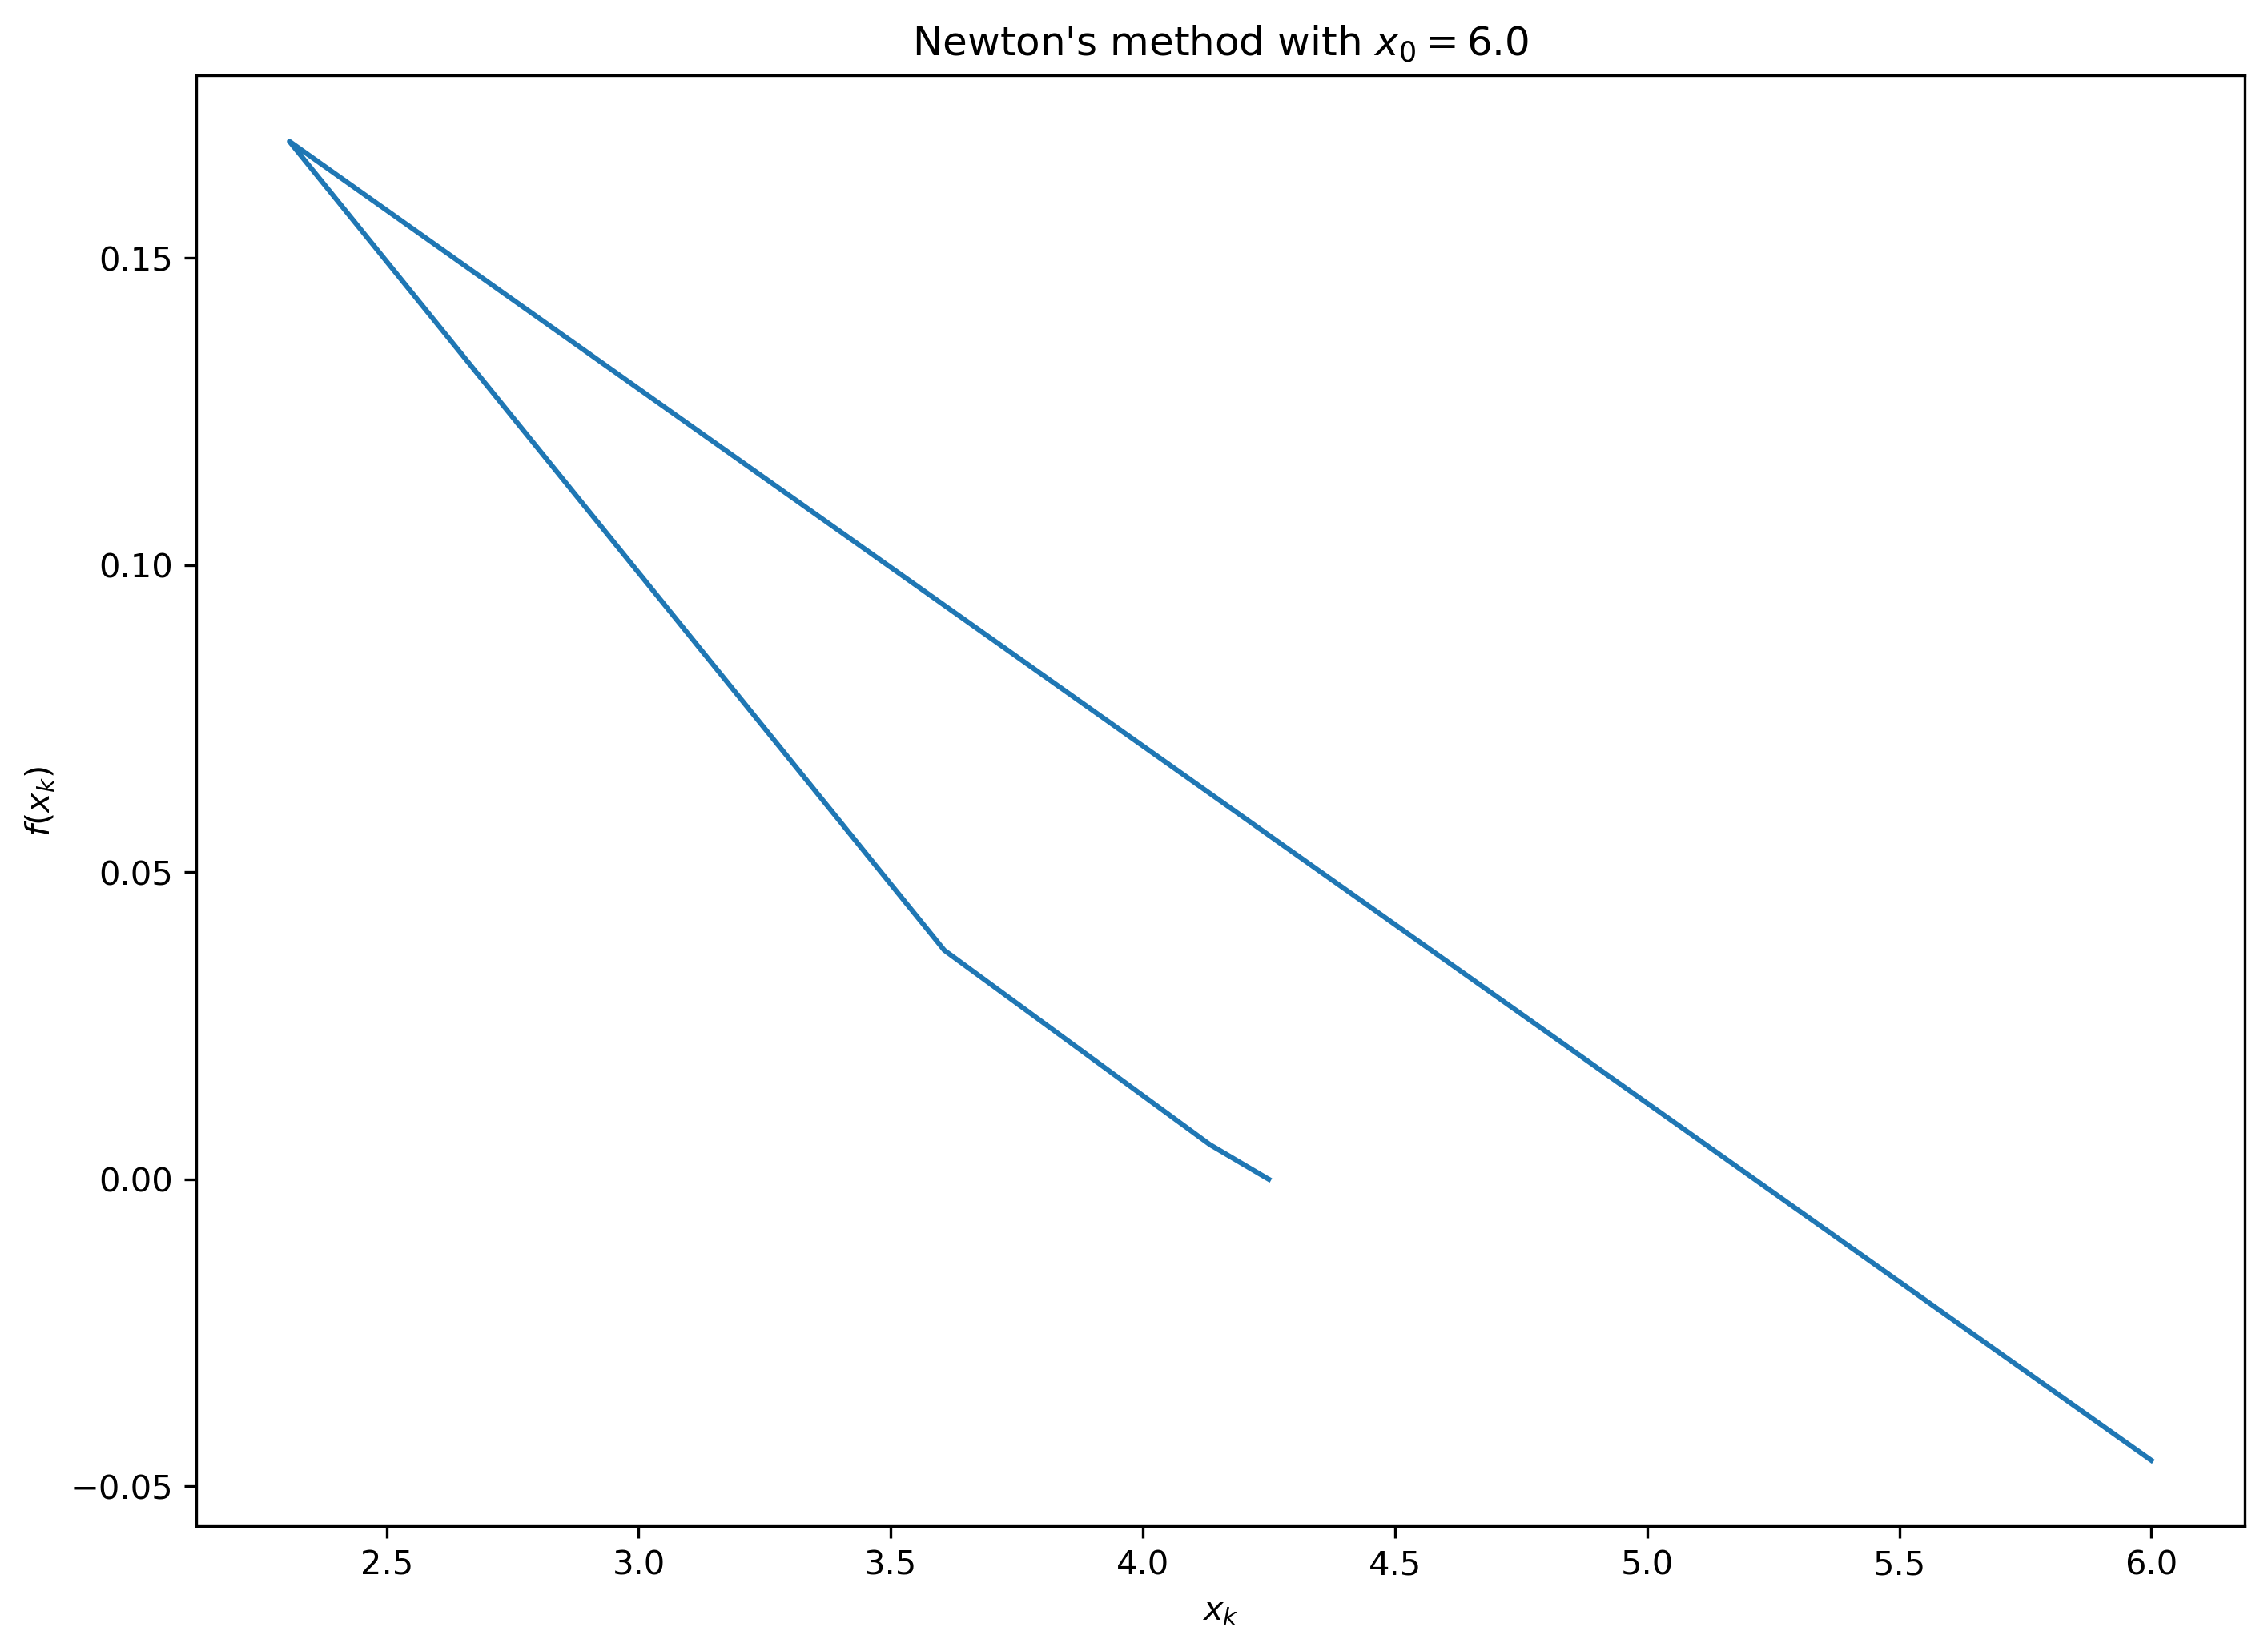
\includegraphics[width=\linewidth]{../figures/Newtons_f_6.0}
	\caption{Function values, $f(x_k)$, versus $x_k$ for each $k$ using Newton's method with $x_0 = 6.0$.}
	\label{fig:newton_f_6.0}
\end{figure}

%%%%%%%%%%%%%%%%%%%%%%%%%%%%%%%%%%%%%%%%%%%%%%%%%%%%%%%%%%%%%%%%%%%%%%%%%%%%%%%%%%%
\subsection{Fixed-point Method Plots - f(x):}

\begin{figure}[H]
	\centering
	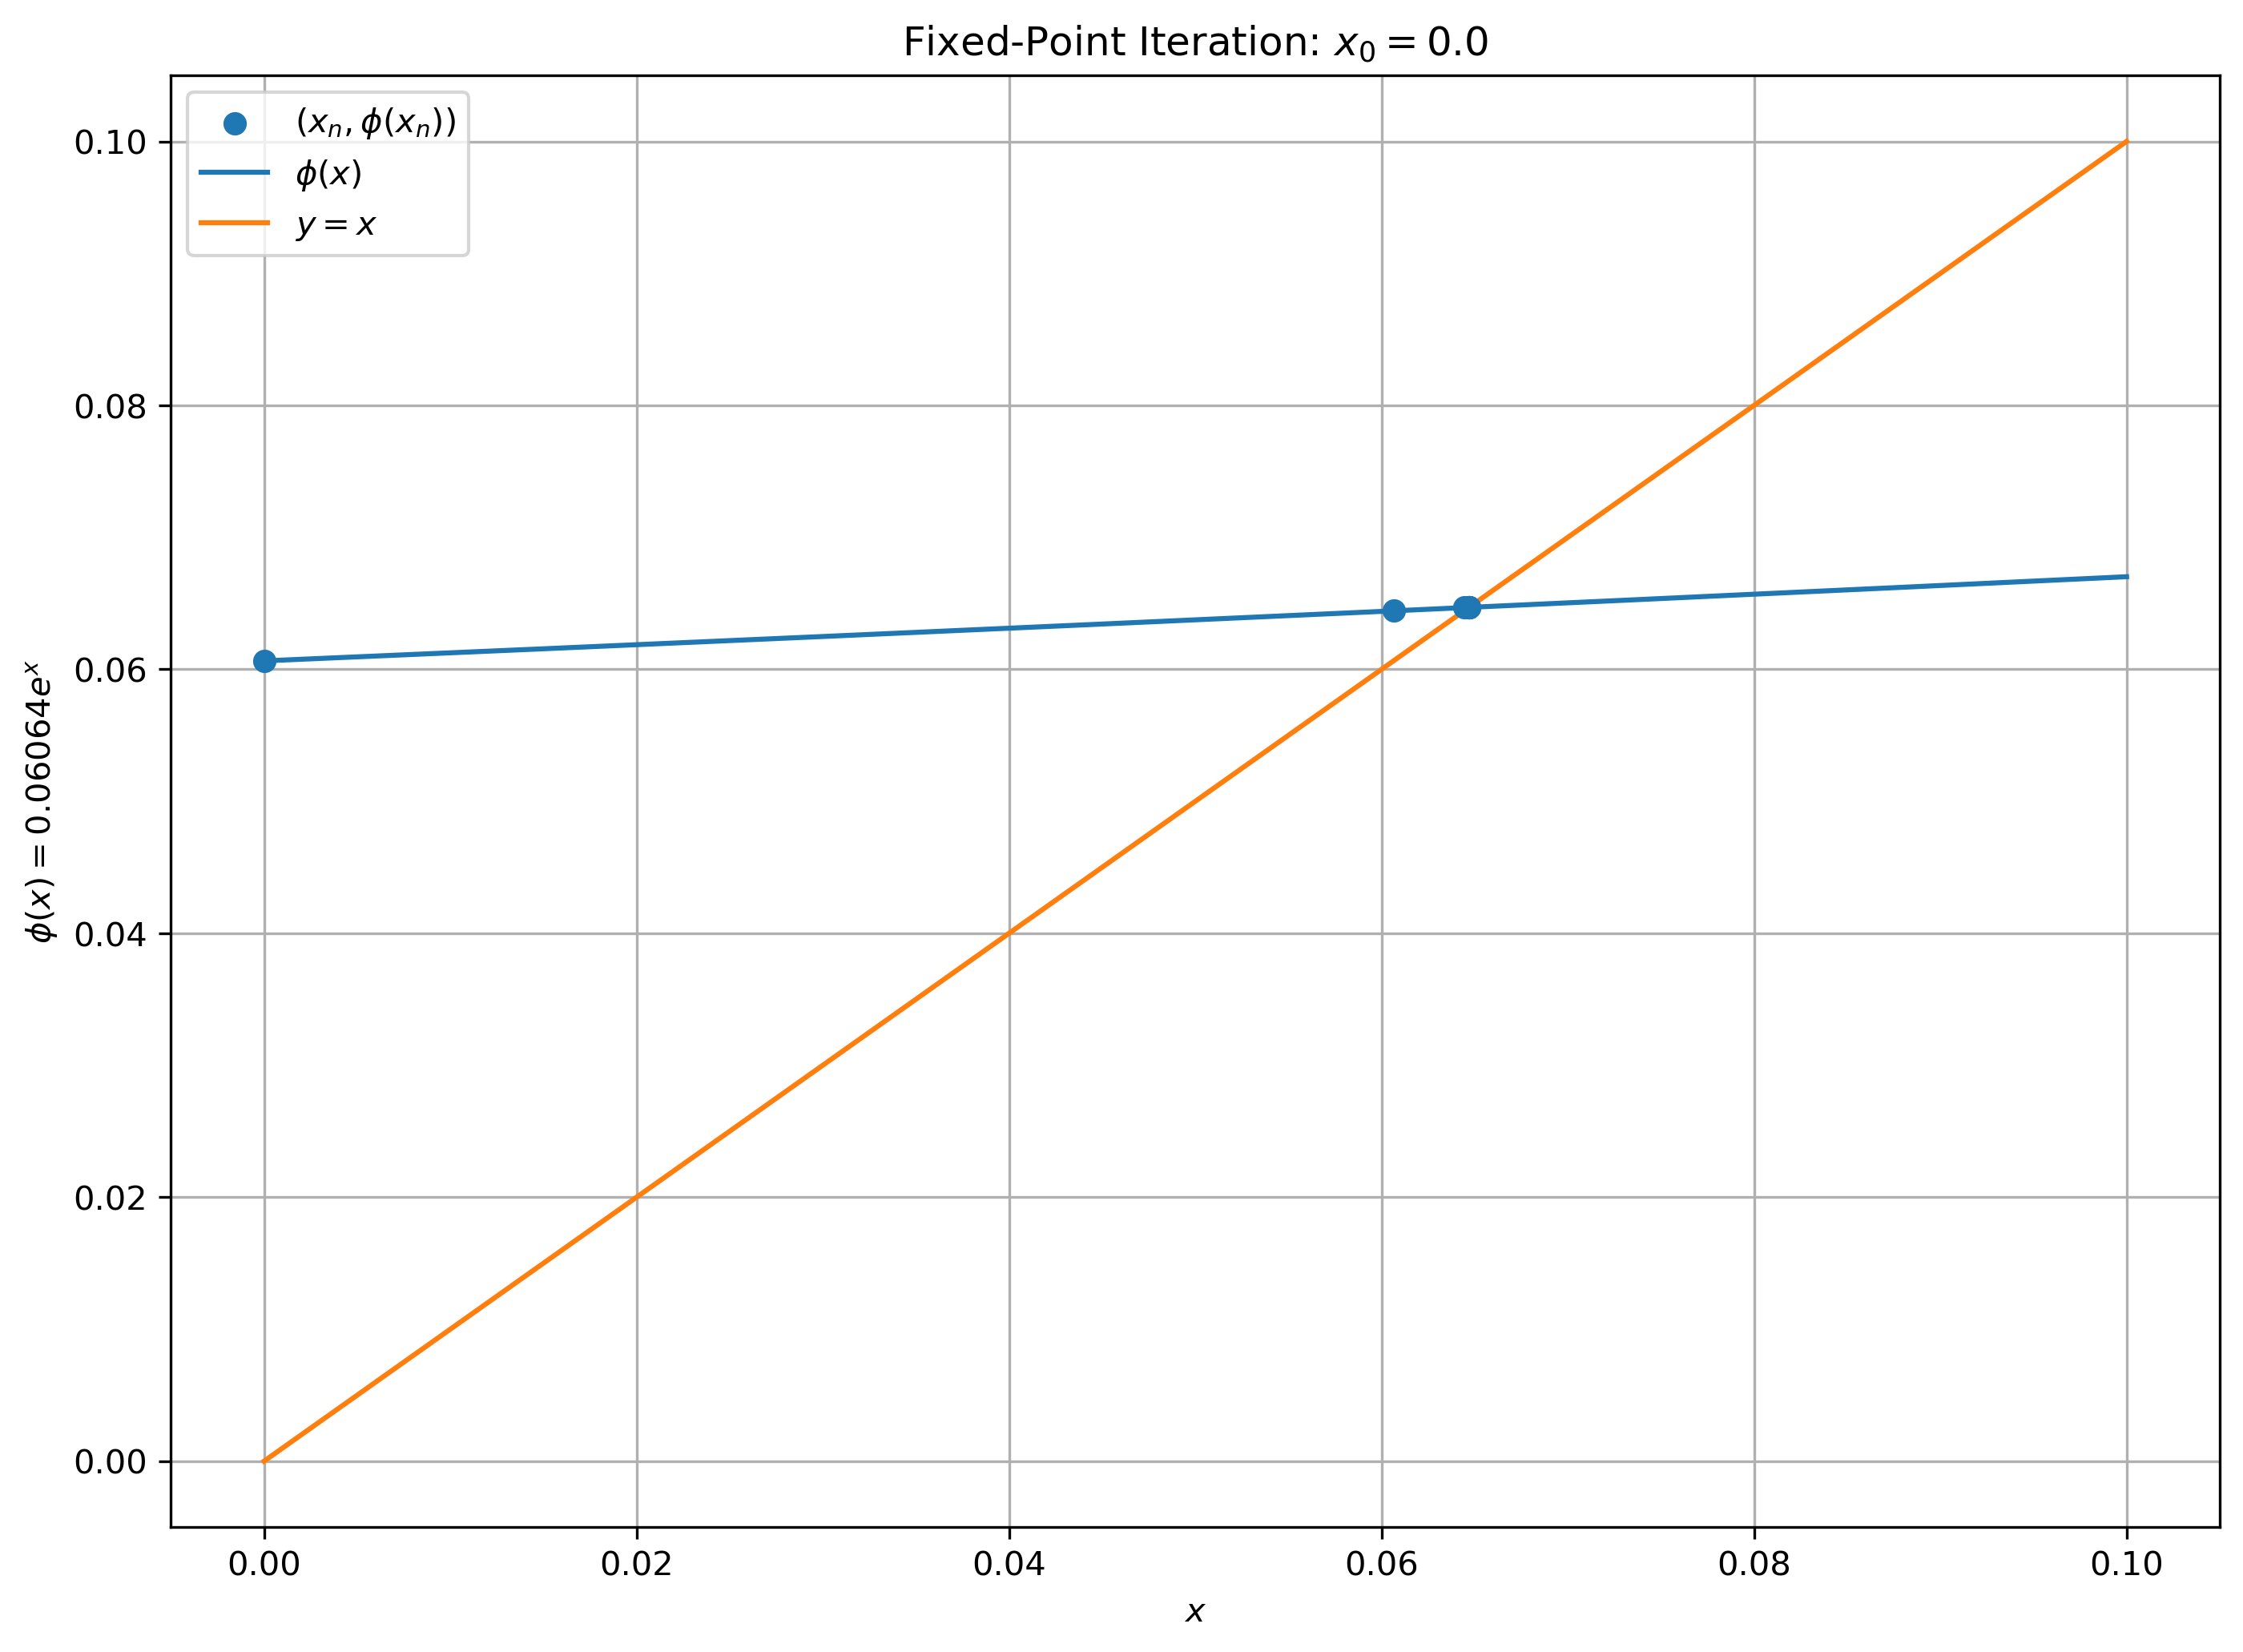
\includegraphics[width=\linewidth]{../figures/Fixed_f_0.0}
	\caption{Fixed-point function values, $\phi(x_k)$, versus $x_k$ for each $k$ using fixed-point method with $x_0 = 0.0$.}
	\label{fig:fixed_f_0.0}
\end{figure}

\begin{figure}[H]
	\centering
	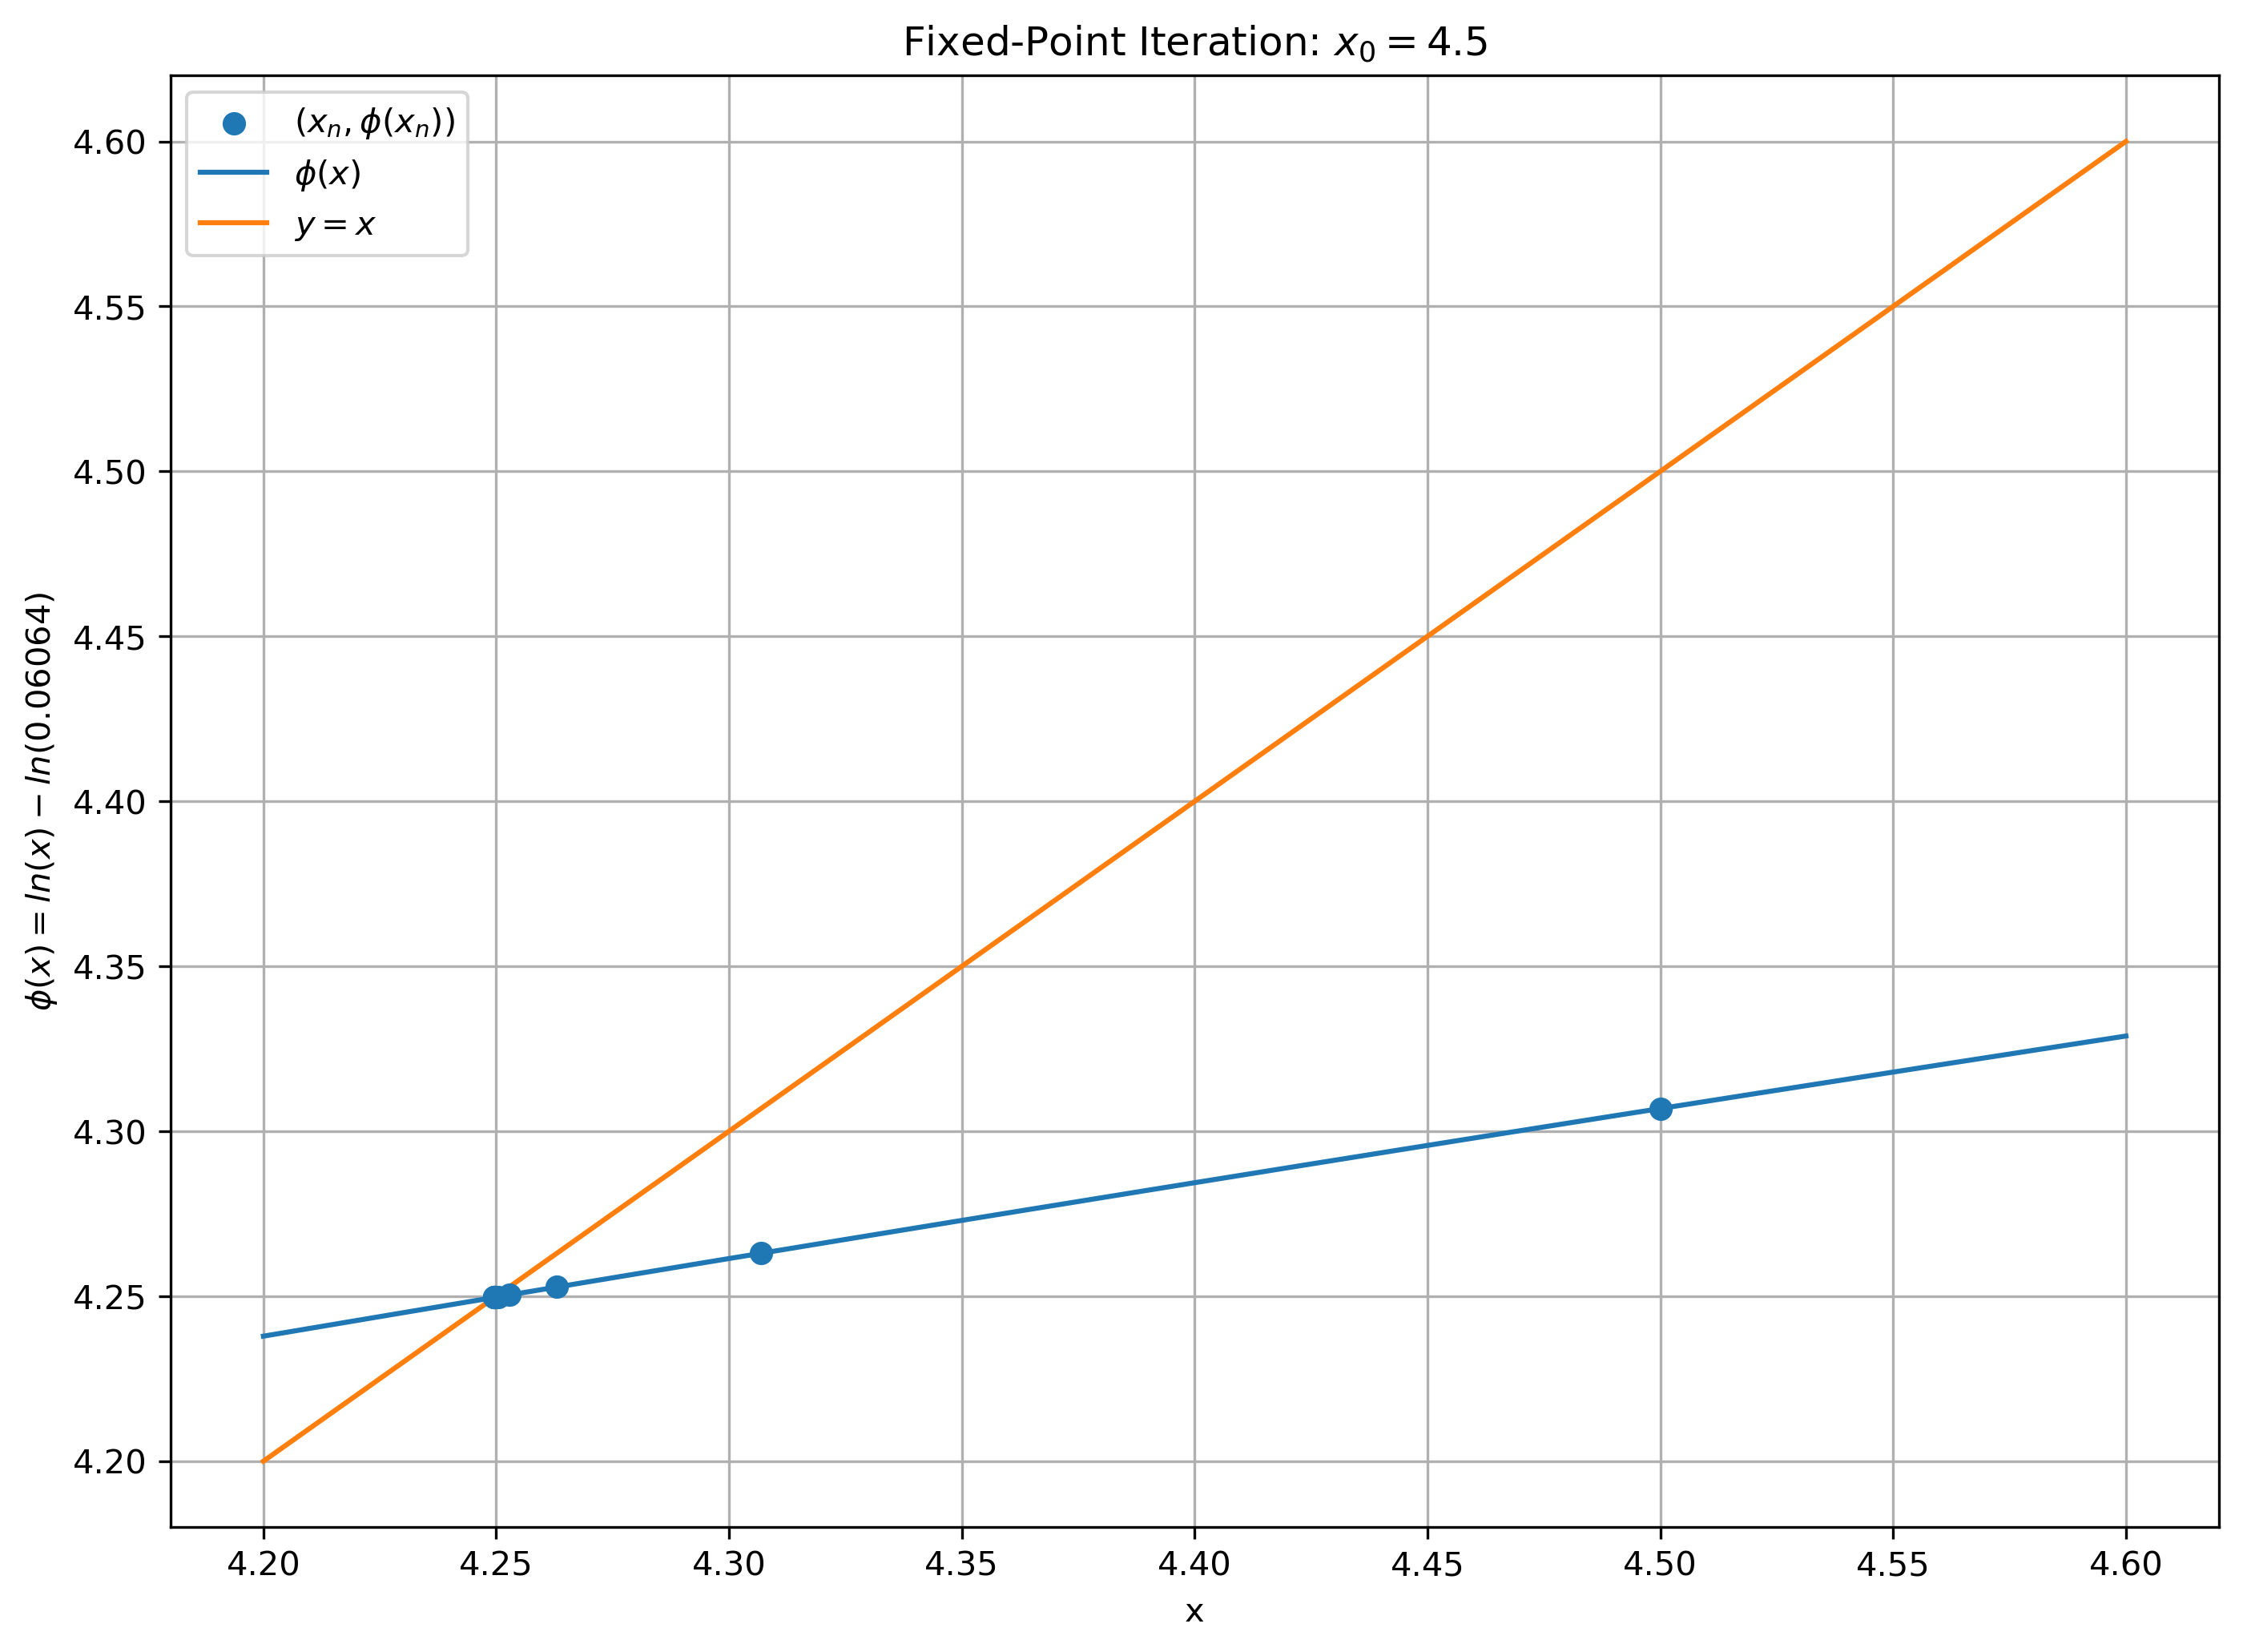
\includegraphics[width=\linewidth]{../figures/Fixed_f_4.5}
	\caption{Fixed-point function values, $\phi(x_k)$, versus $x_k$ for each $k$ using fixed-point method with $x_0 = 0.0$.}
	\label{fig:fixed_f_4.5}
\end{figure}

%%%%%%%%%%%%%%%%%%%%%%%%%%%%%%%%%%%%%%%%%%%%%%%%%%%%%%%%%%%%%%%%%%%%%%%%%%%%%%%%%%%
%%%%%%%%%%%%%%%%%%%%%%%%%%%%%%%%%%%%%%%%%%%%%%%%%%%%%%%%%%%%%%%%%%%%%%%%%%%%%%%%%%%

\subsection{Bisection Plots - g(x):}
\begin{figure}[H]
	\centering
	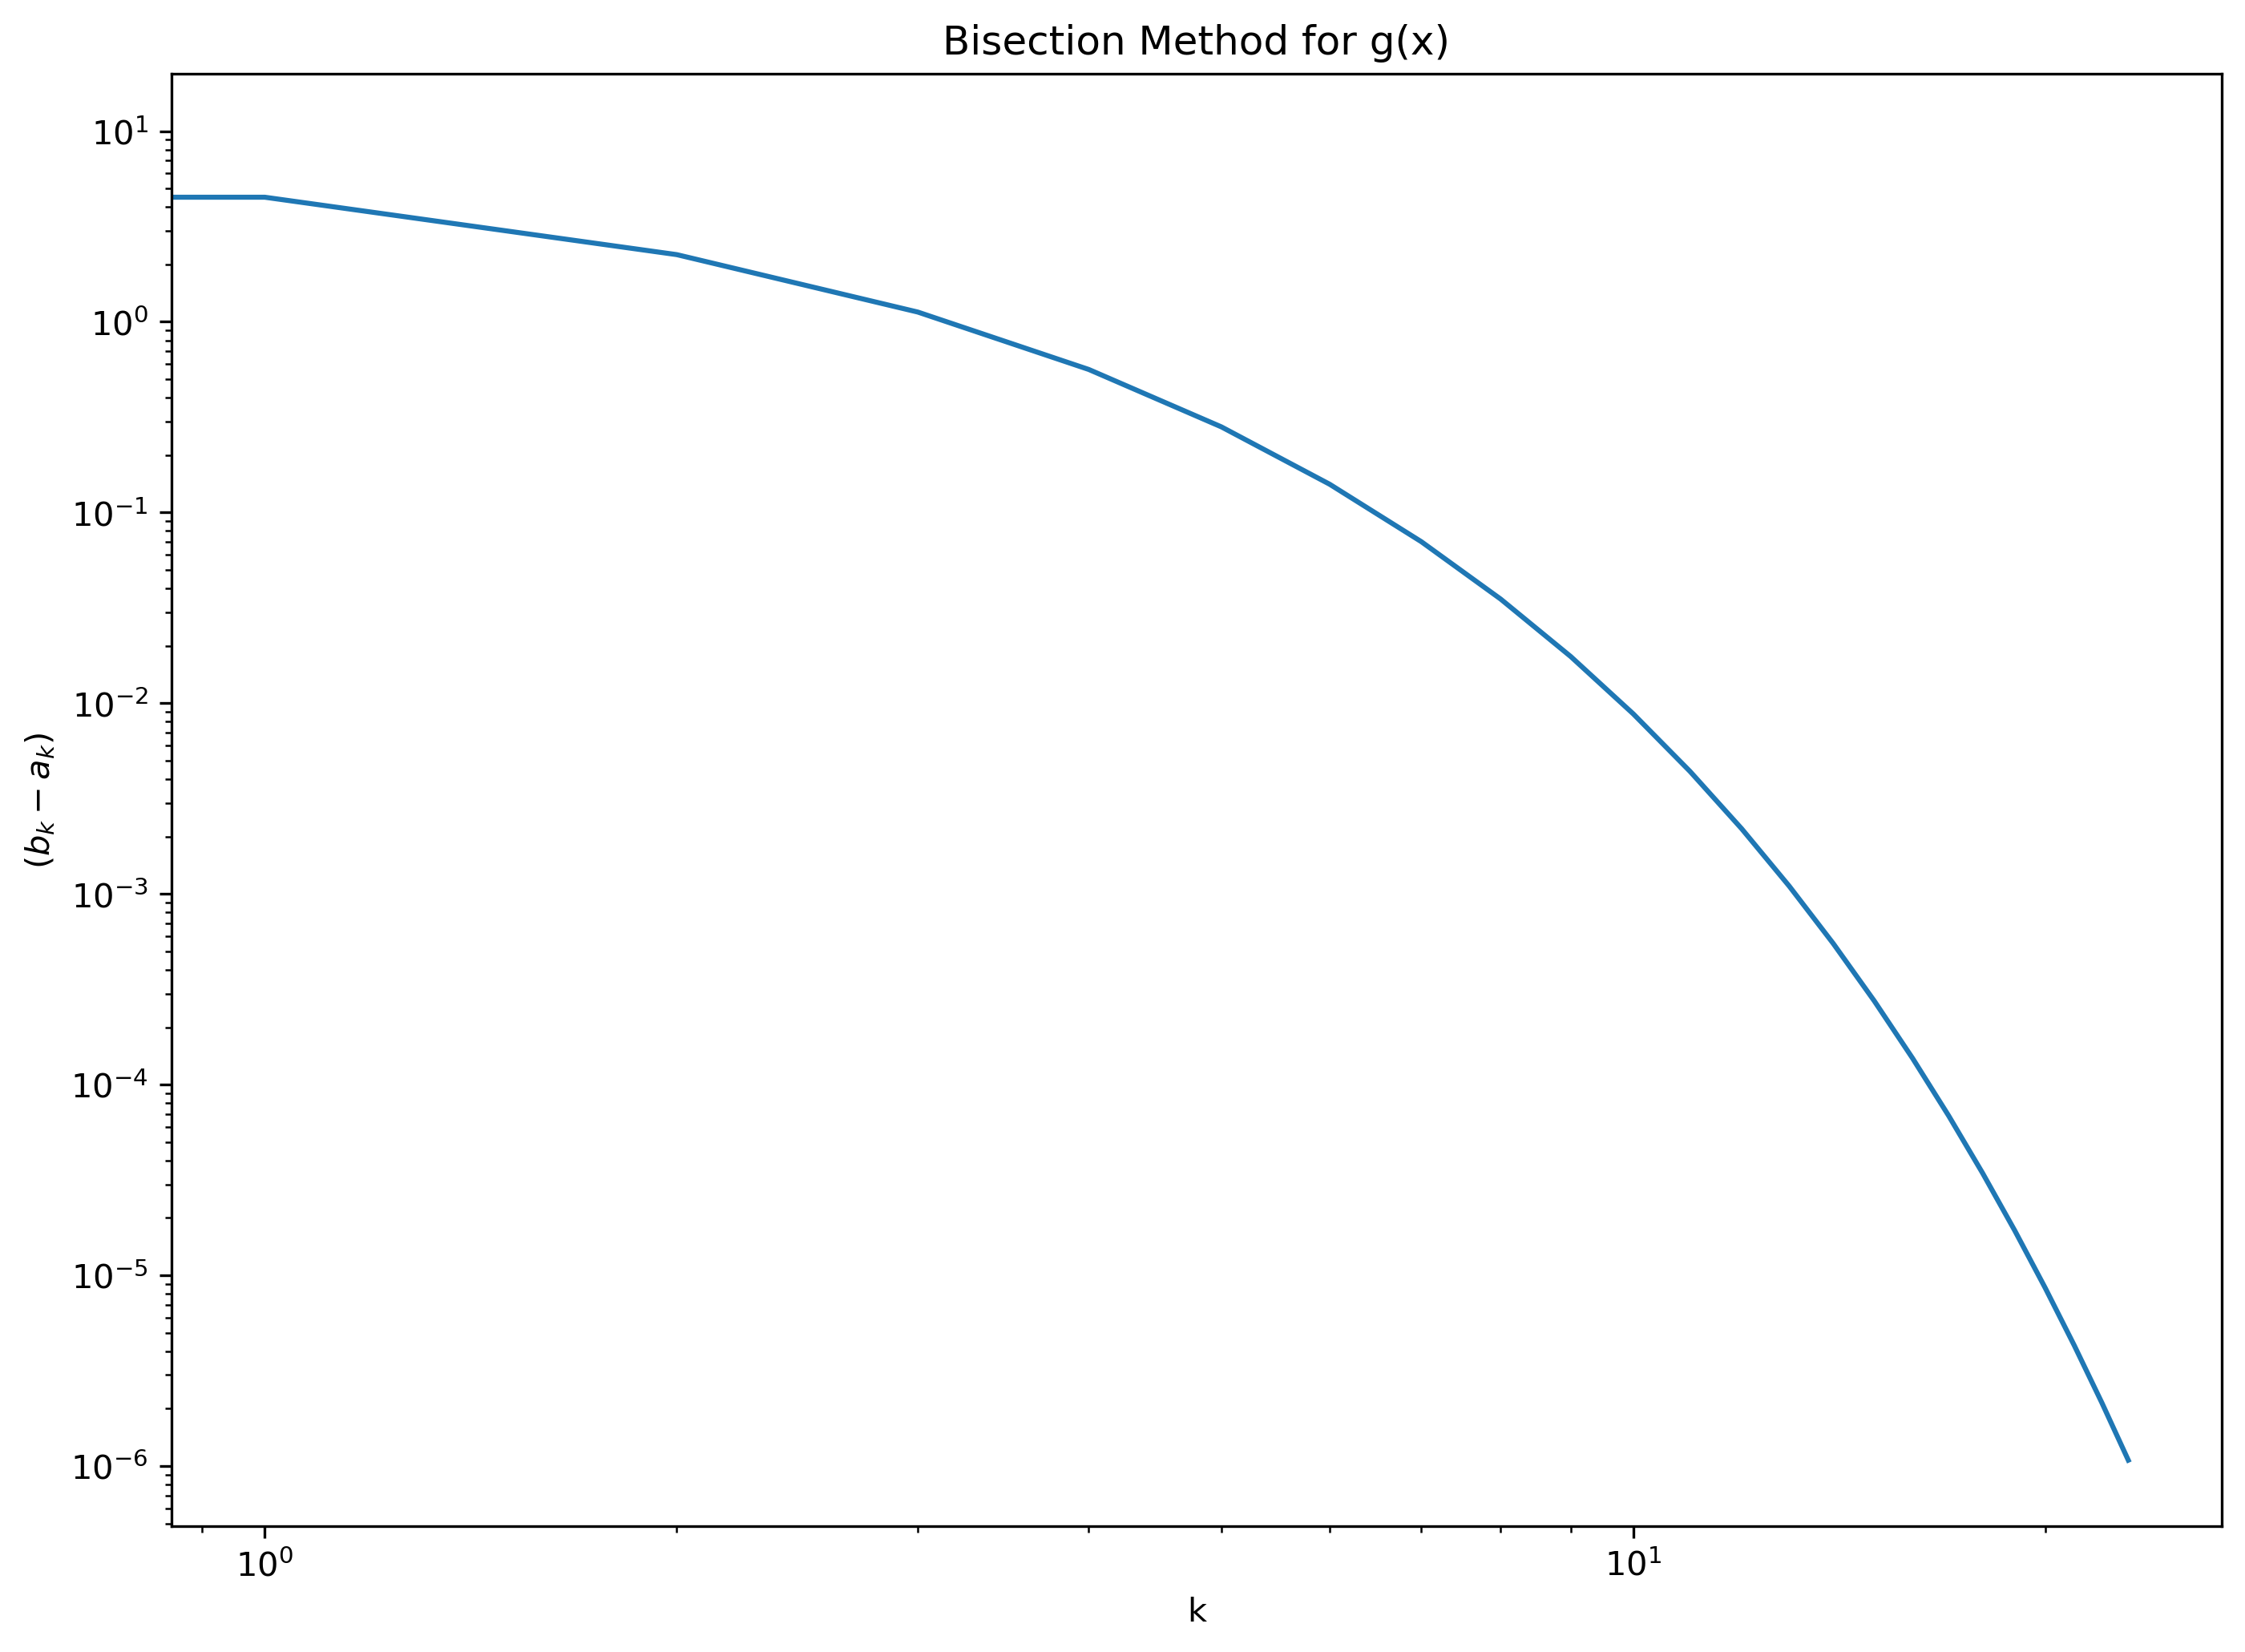
\includegraphics[width=\linewidth]{../figures/Bisection_g}
	\caption{Interval size per iteration step for the first root of $g(x) = x^3 - x - 6$ using the bisection method, shown in logscale.}
	\label{fig:bisec_g}
\end{figure}

\begin{figure}[H]
	\centering
	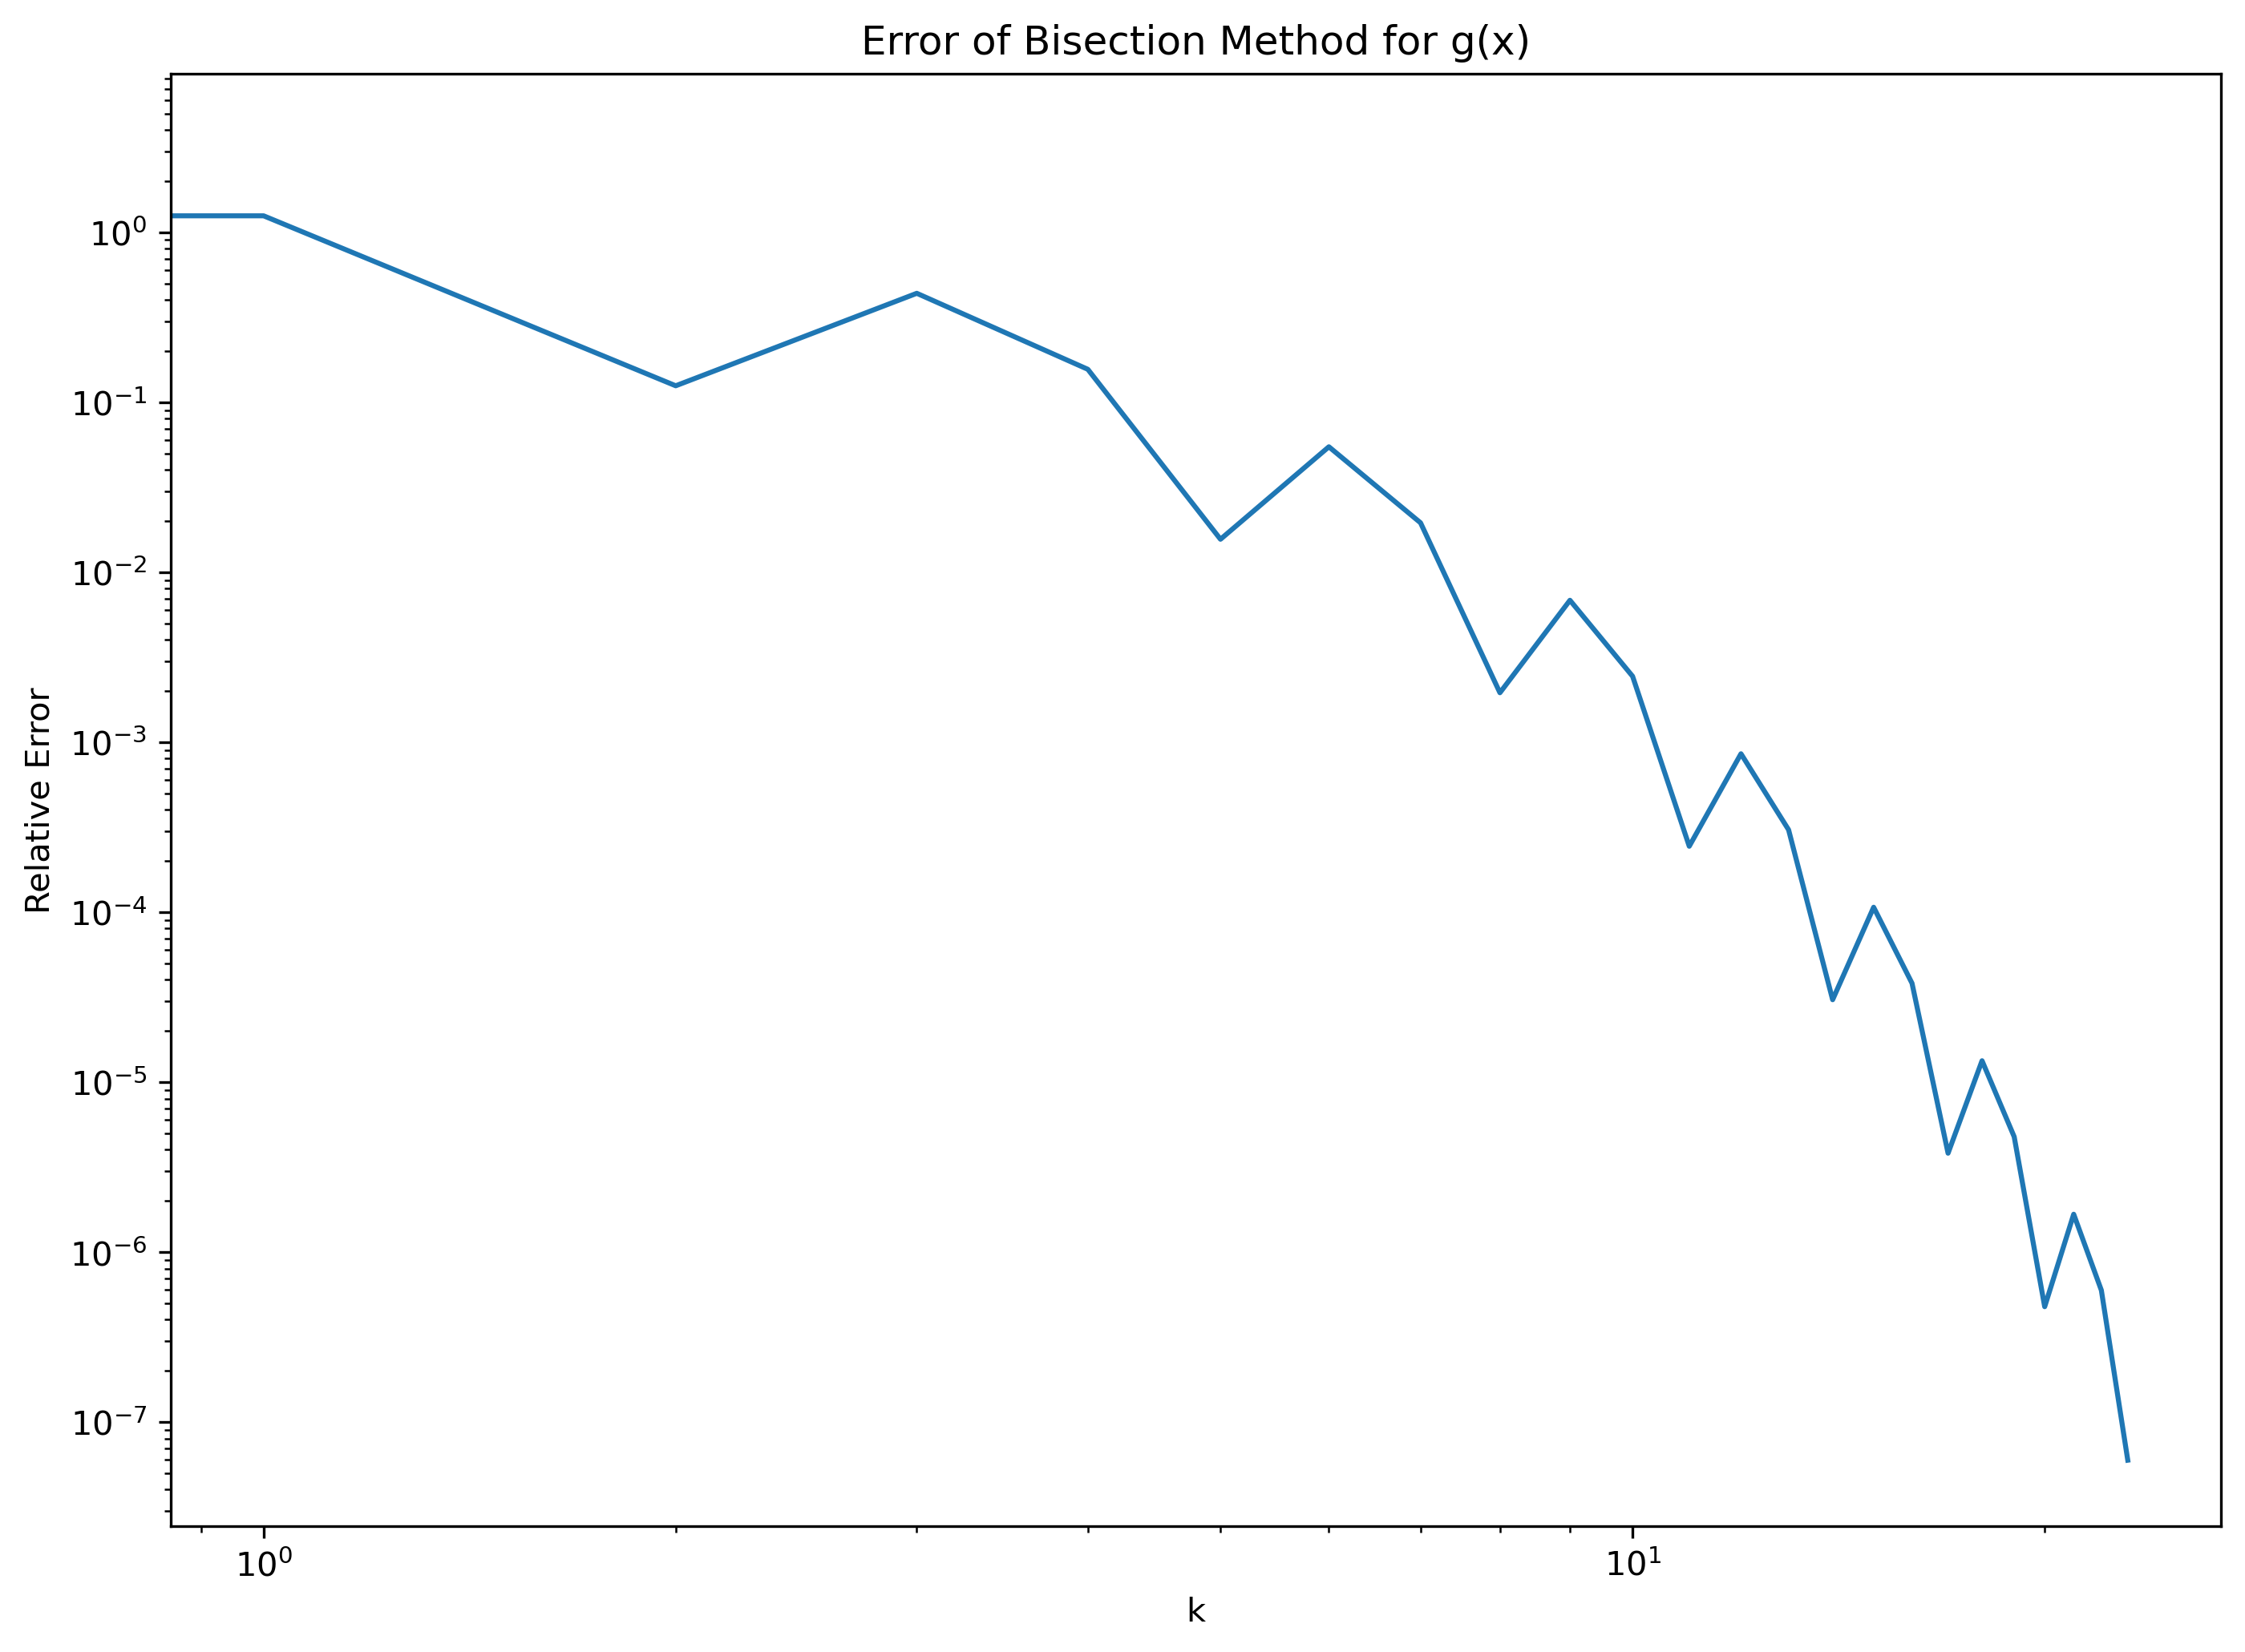
\includegraphics[width=\linewidth]{../figures/Bisection_g_err}
	\caption{Error achieved per iteration step for the root of $g(x) = x^3 - x - 6$ using the bisection method, shown in logscale.}
	\label{fig:bisec_g_err}
\end{figure}

%%%%%%%%%%%%%%%%%%%%%%%%%%%%%%%%%%%%%%%%%%%%%%%%%%%%%%%%%%%%%%%%%%%%%%%%%%%%%%%%%%%

\subsection{Newton's Method Plots - g(x):}
\begin{figure}[H]
	\centering
	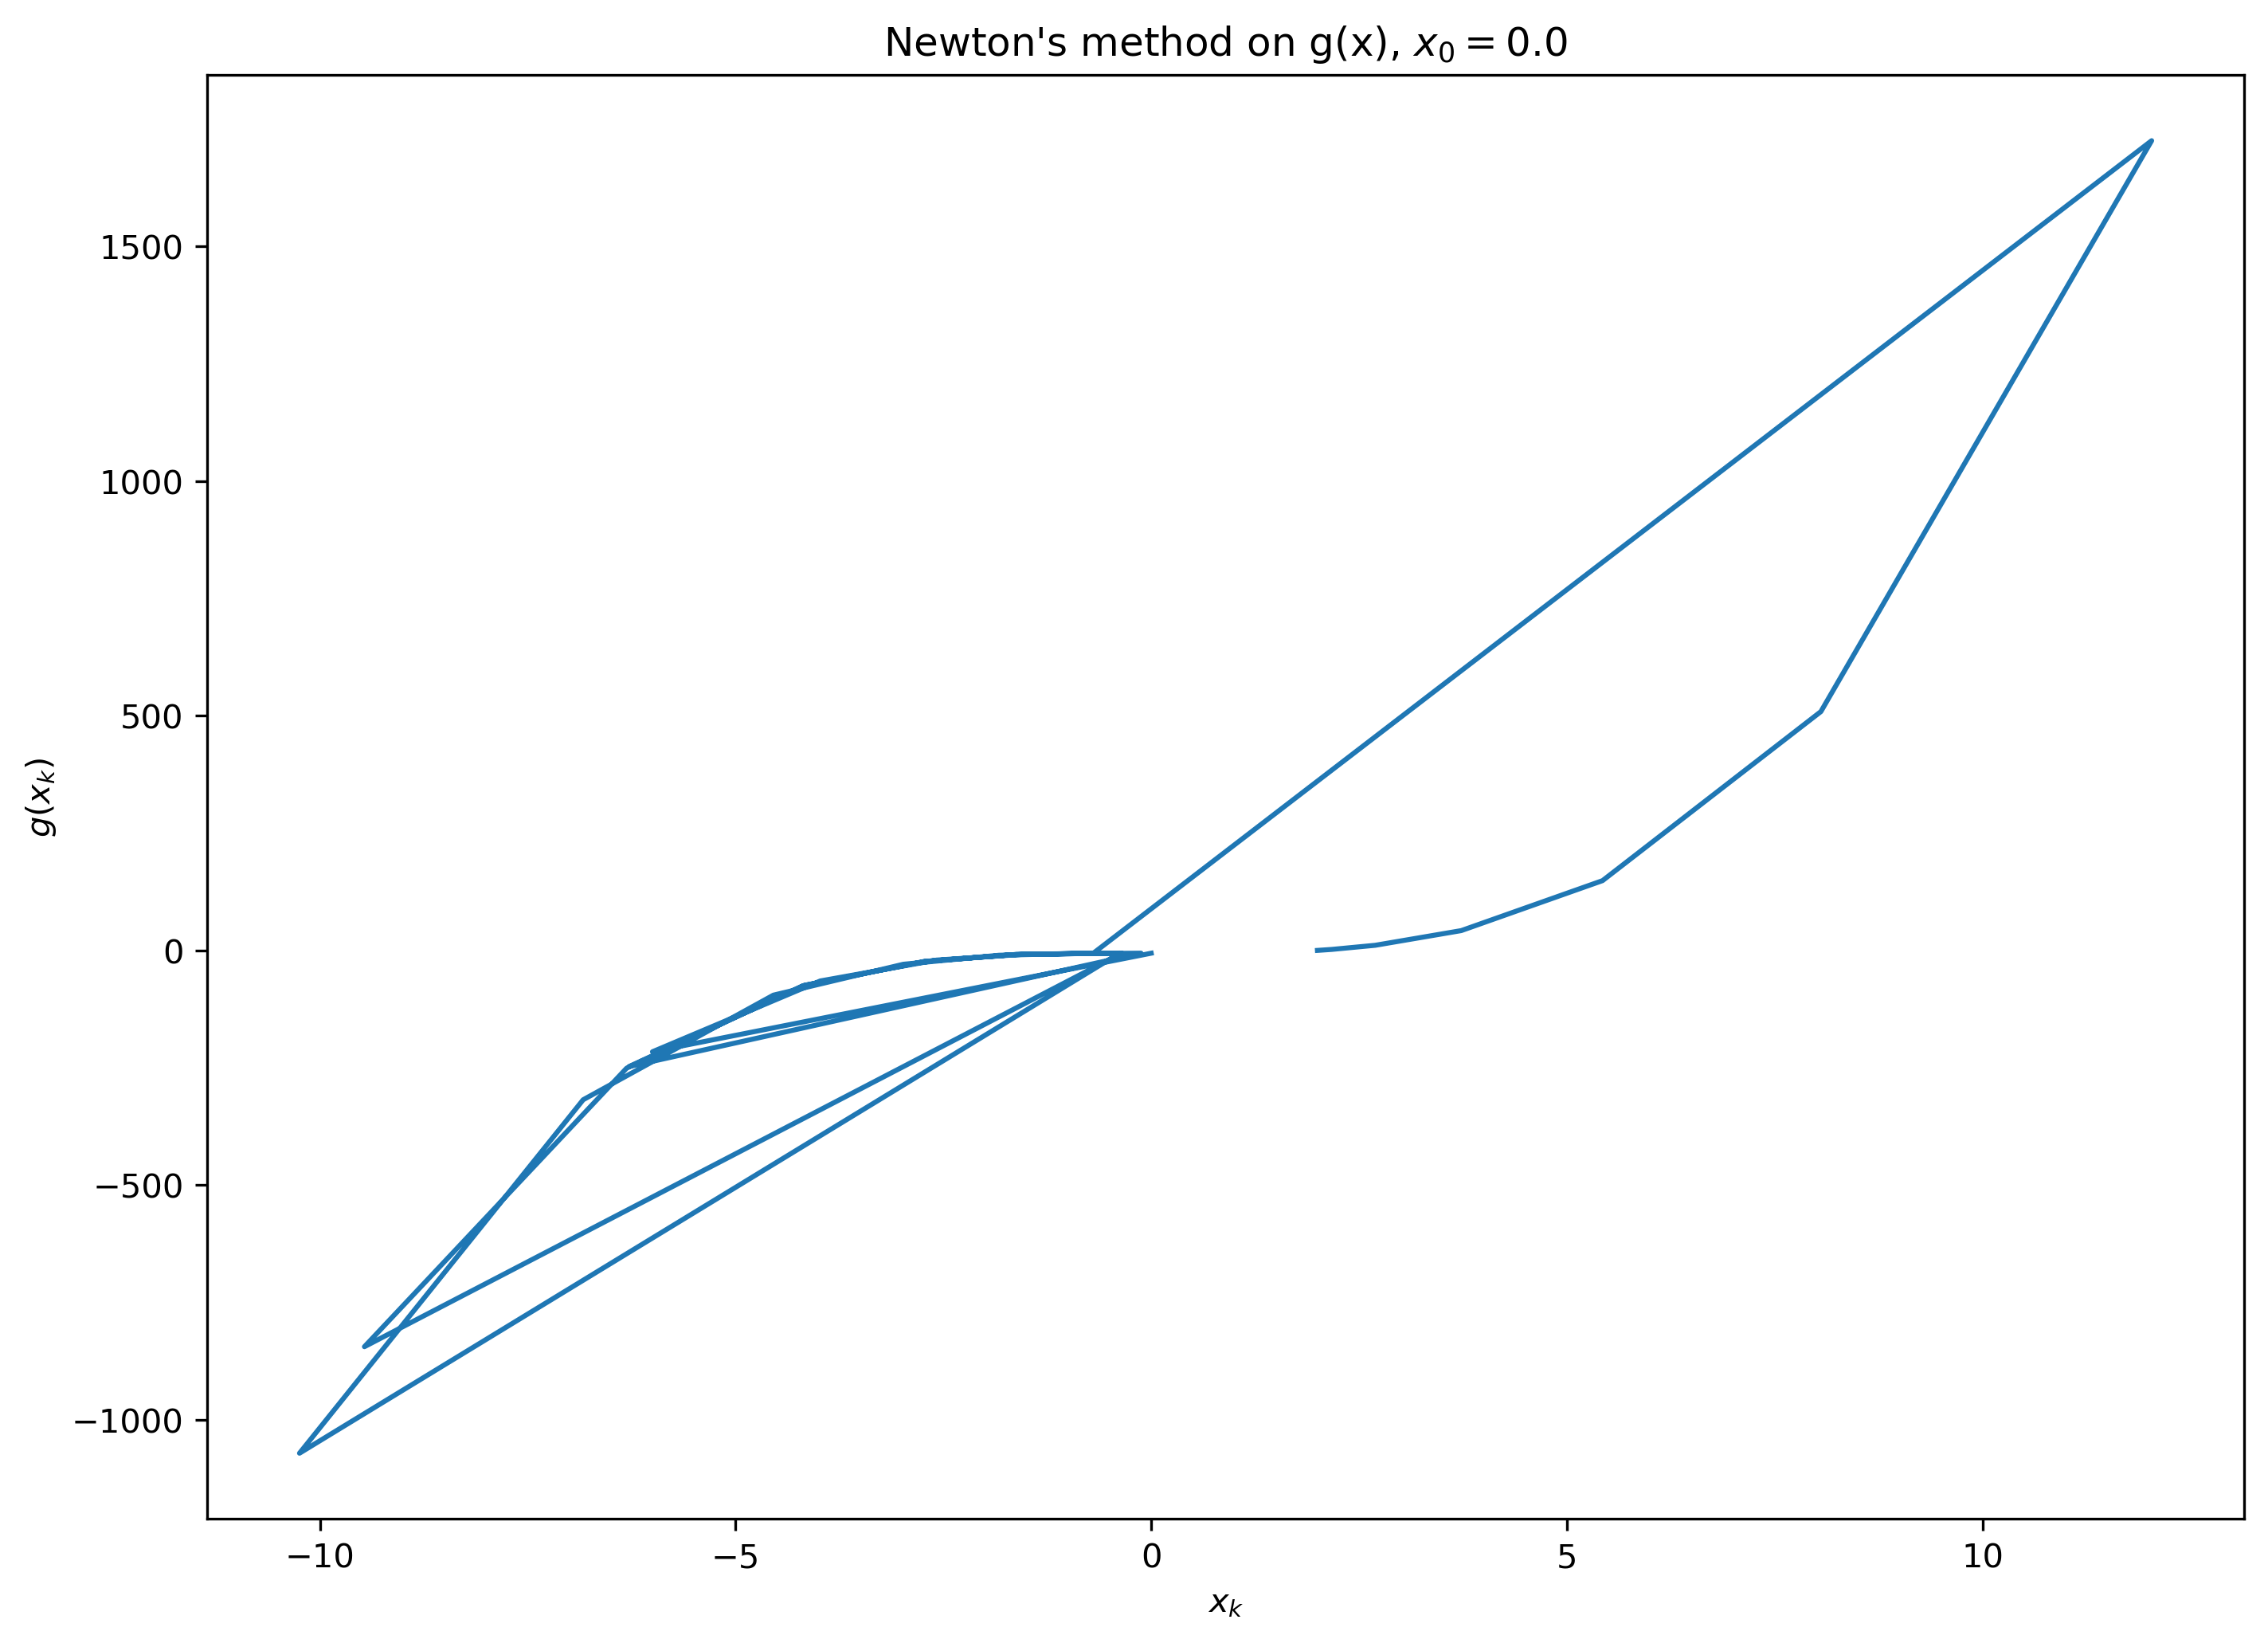
\includegraphics[width=\linewidth]{../figures/Newtons_g_0.0}
	\caption{Function values, $g(x_k)$, versus $x_k$ for each $k$ using Newton's method with $x_0 = 0.0$.}
	\label{fig:newton_g_0.0}
\end{figure}

\begin{figure}[H]
	\centering
	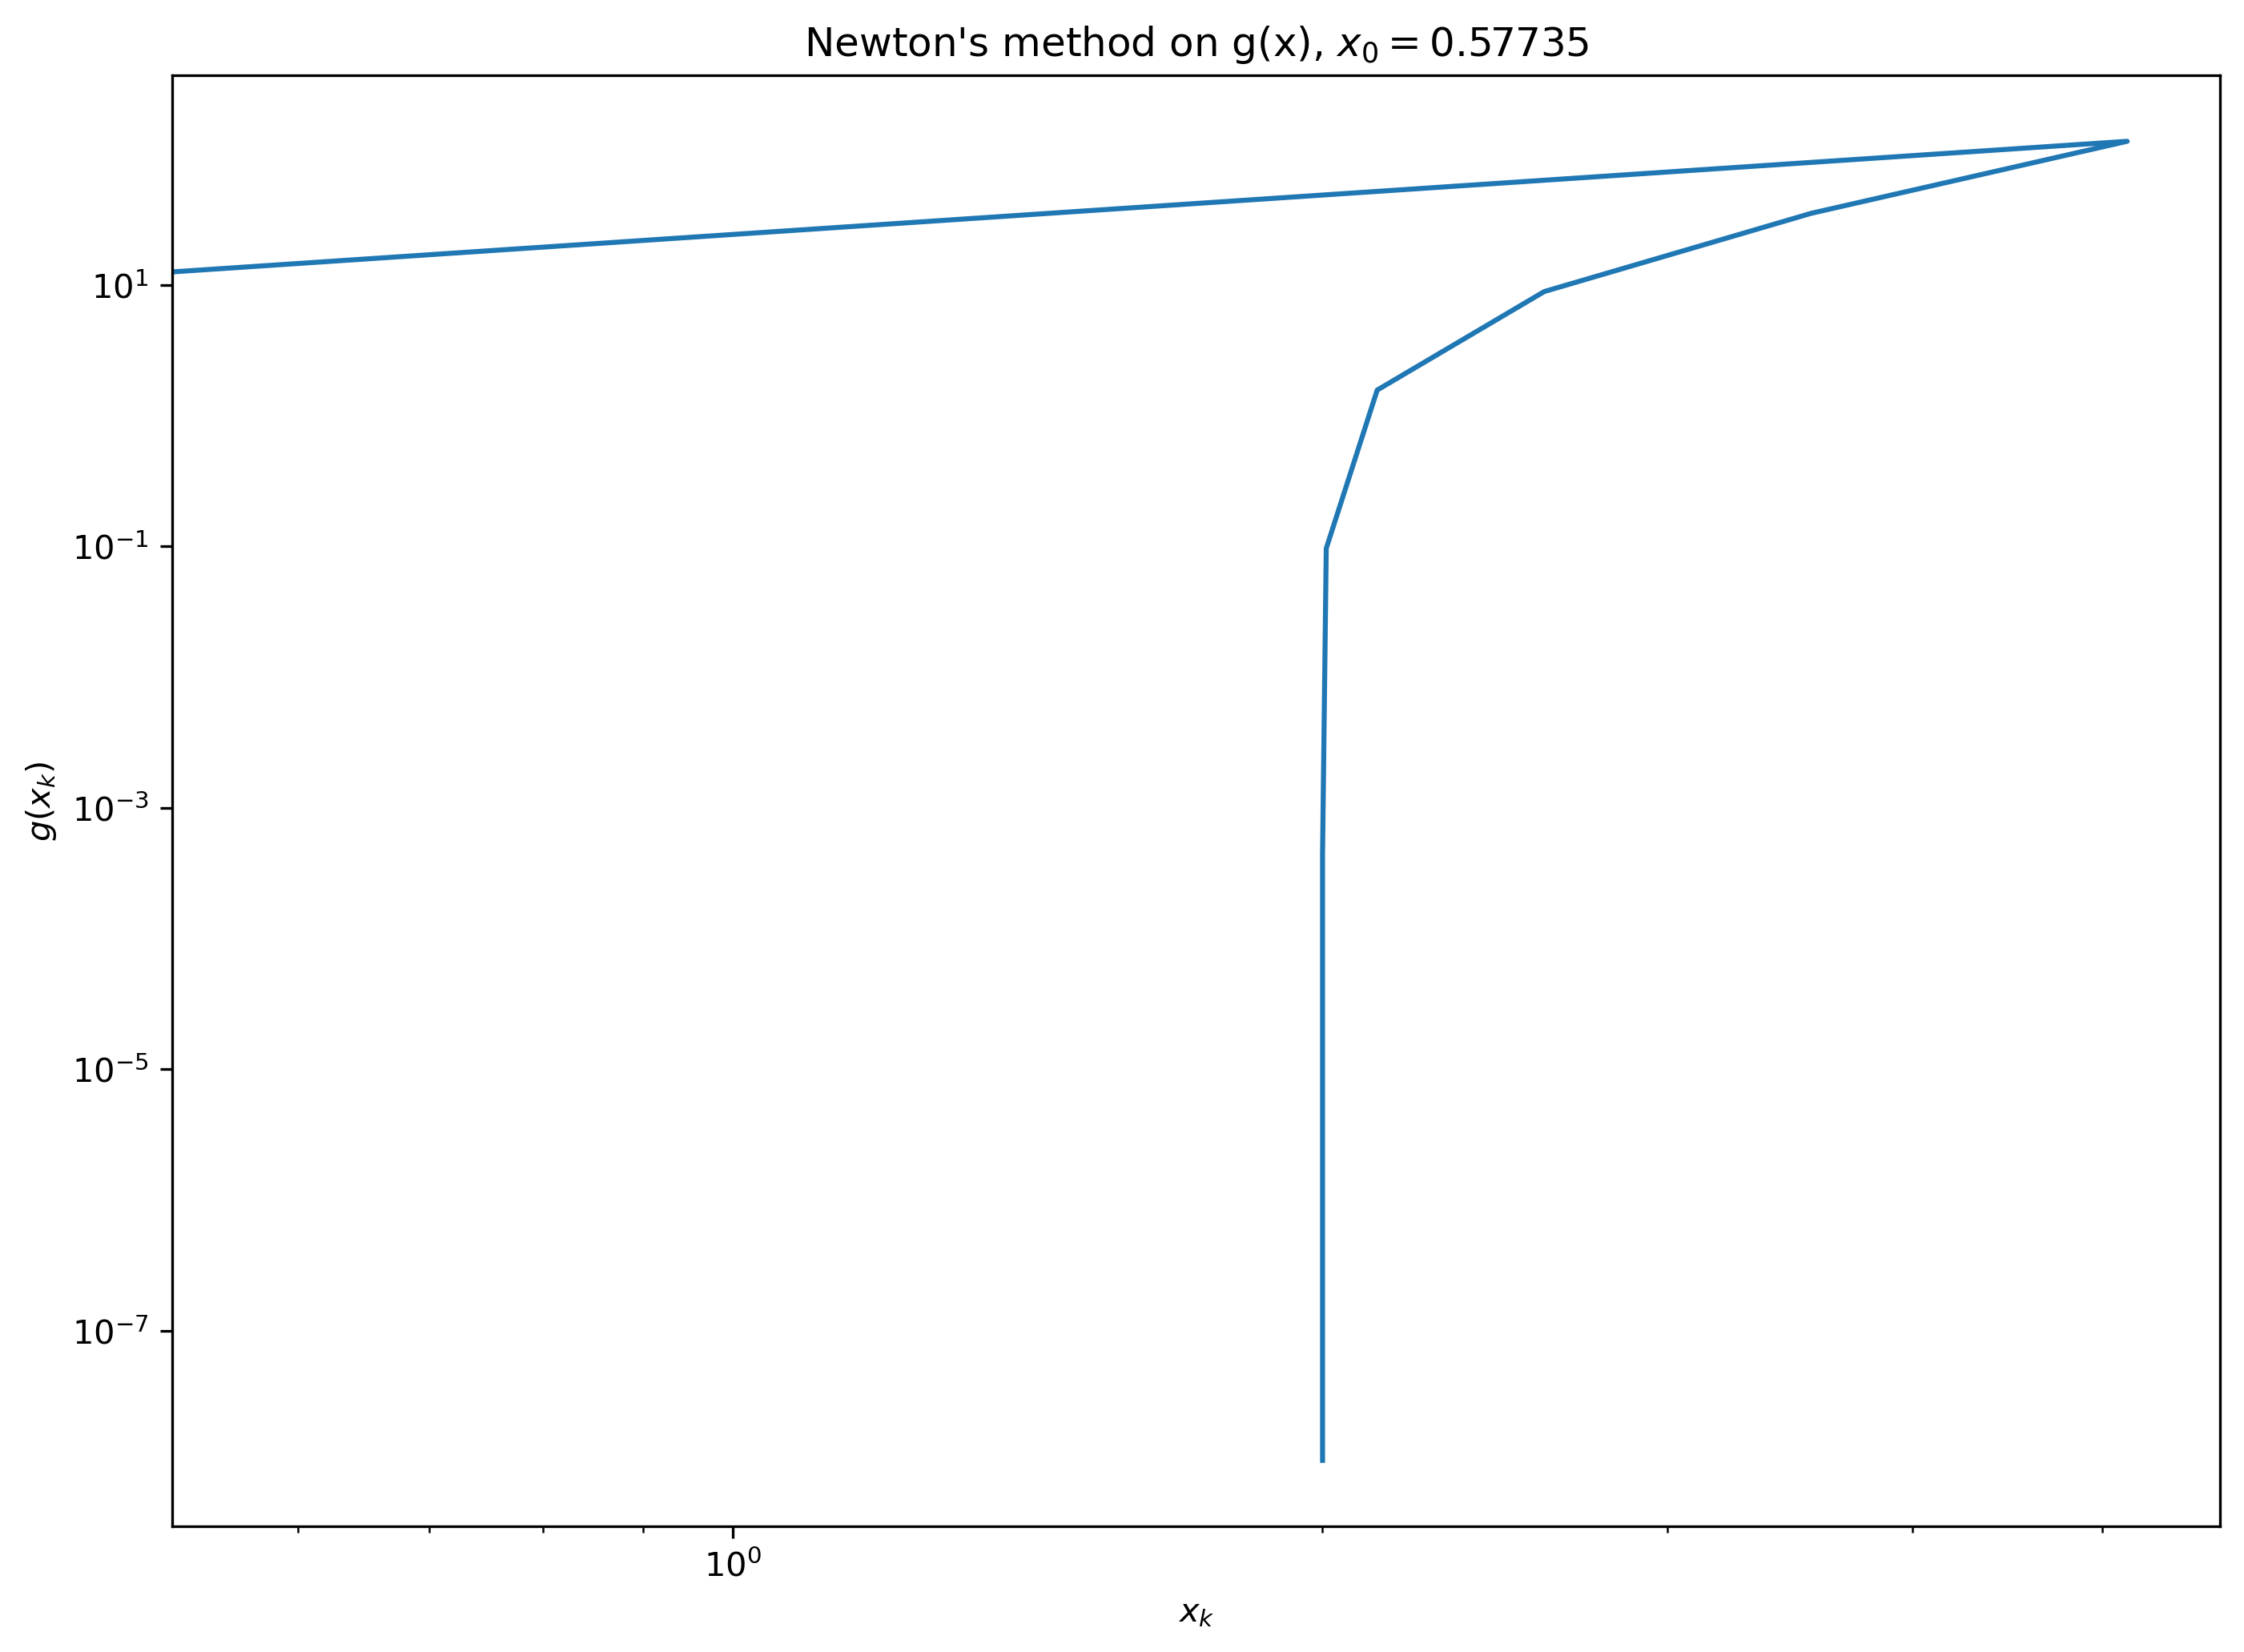
\includegraphics[width=\linewidth]{../figures/Newtons_g_0.57735}
	\caption{Function values, $g(x_k)$, versus $x_k$ for each $k$ using Newton's method with $x_0 = 0.57735$, shown in logscale.}
	\label{fig:newton_g_0.57735}
\end{figure}

\begin{figure}[H]
	\centering
	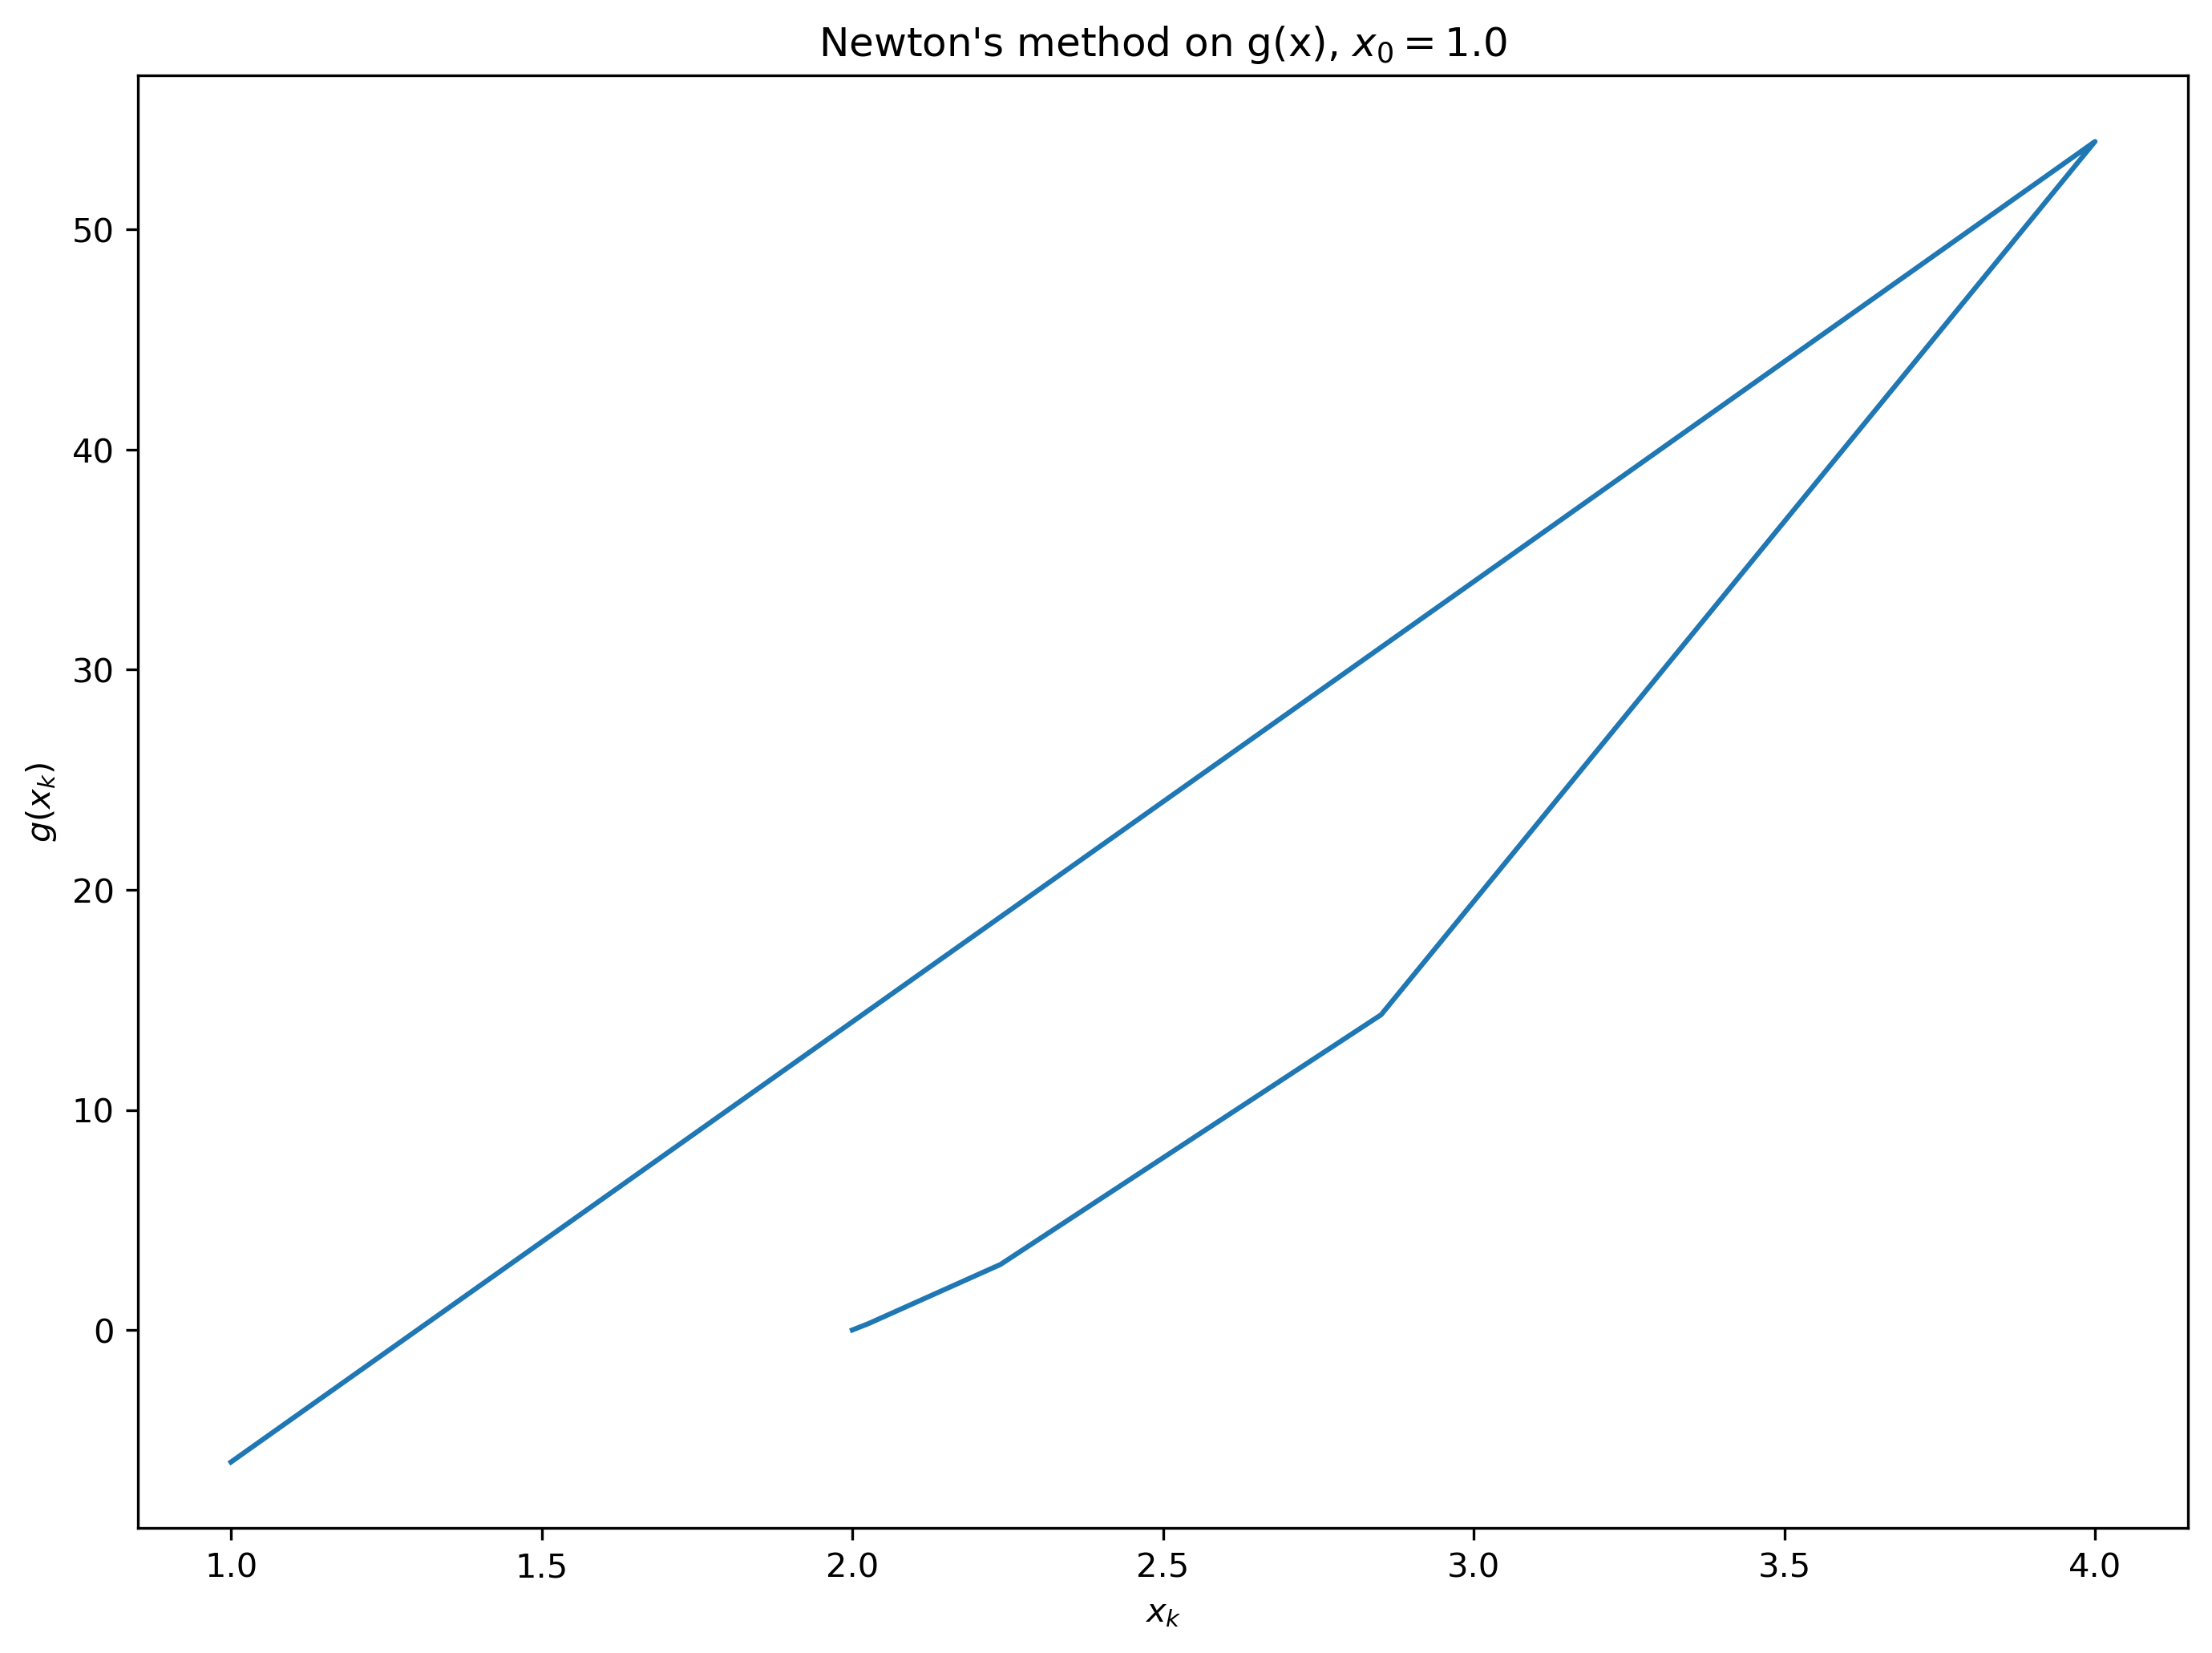
\includegraphics[width=\linewidth]{../figures/Newtons_g_1.0}
	\caption{Function values, $g(x_k)$, versus $x_k$ for each $k$ using Newton's method with $x_0 = 1.0$.}
	\label{fig:newton_g_1.0}
\end{figure}

\begin{figure}[H]
	\centering
	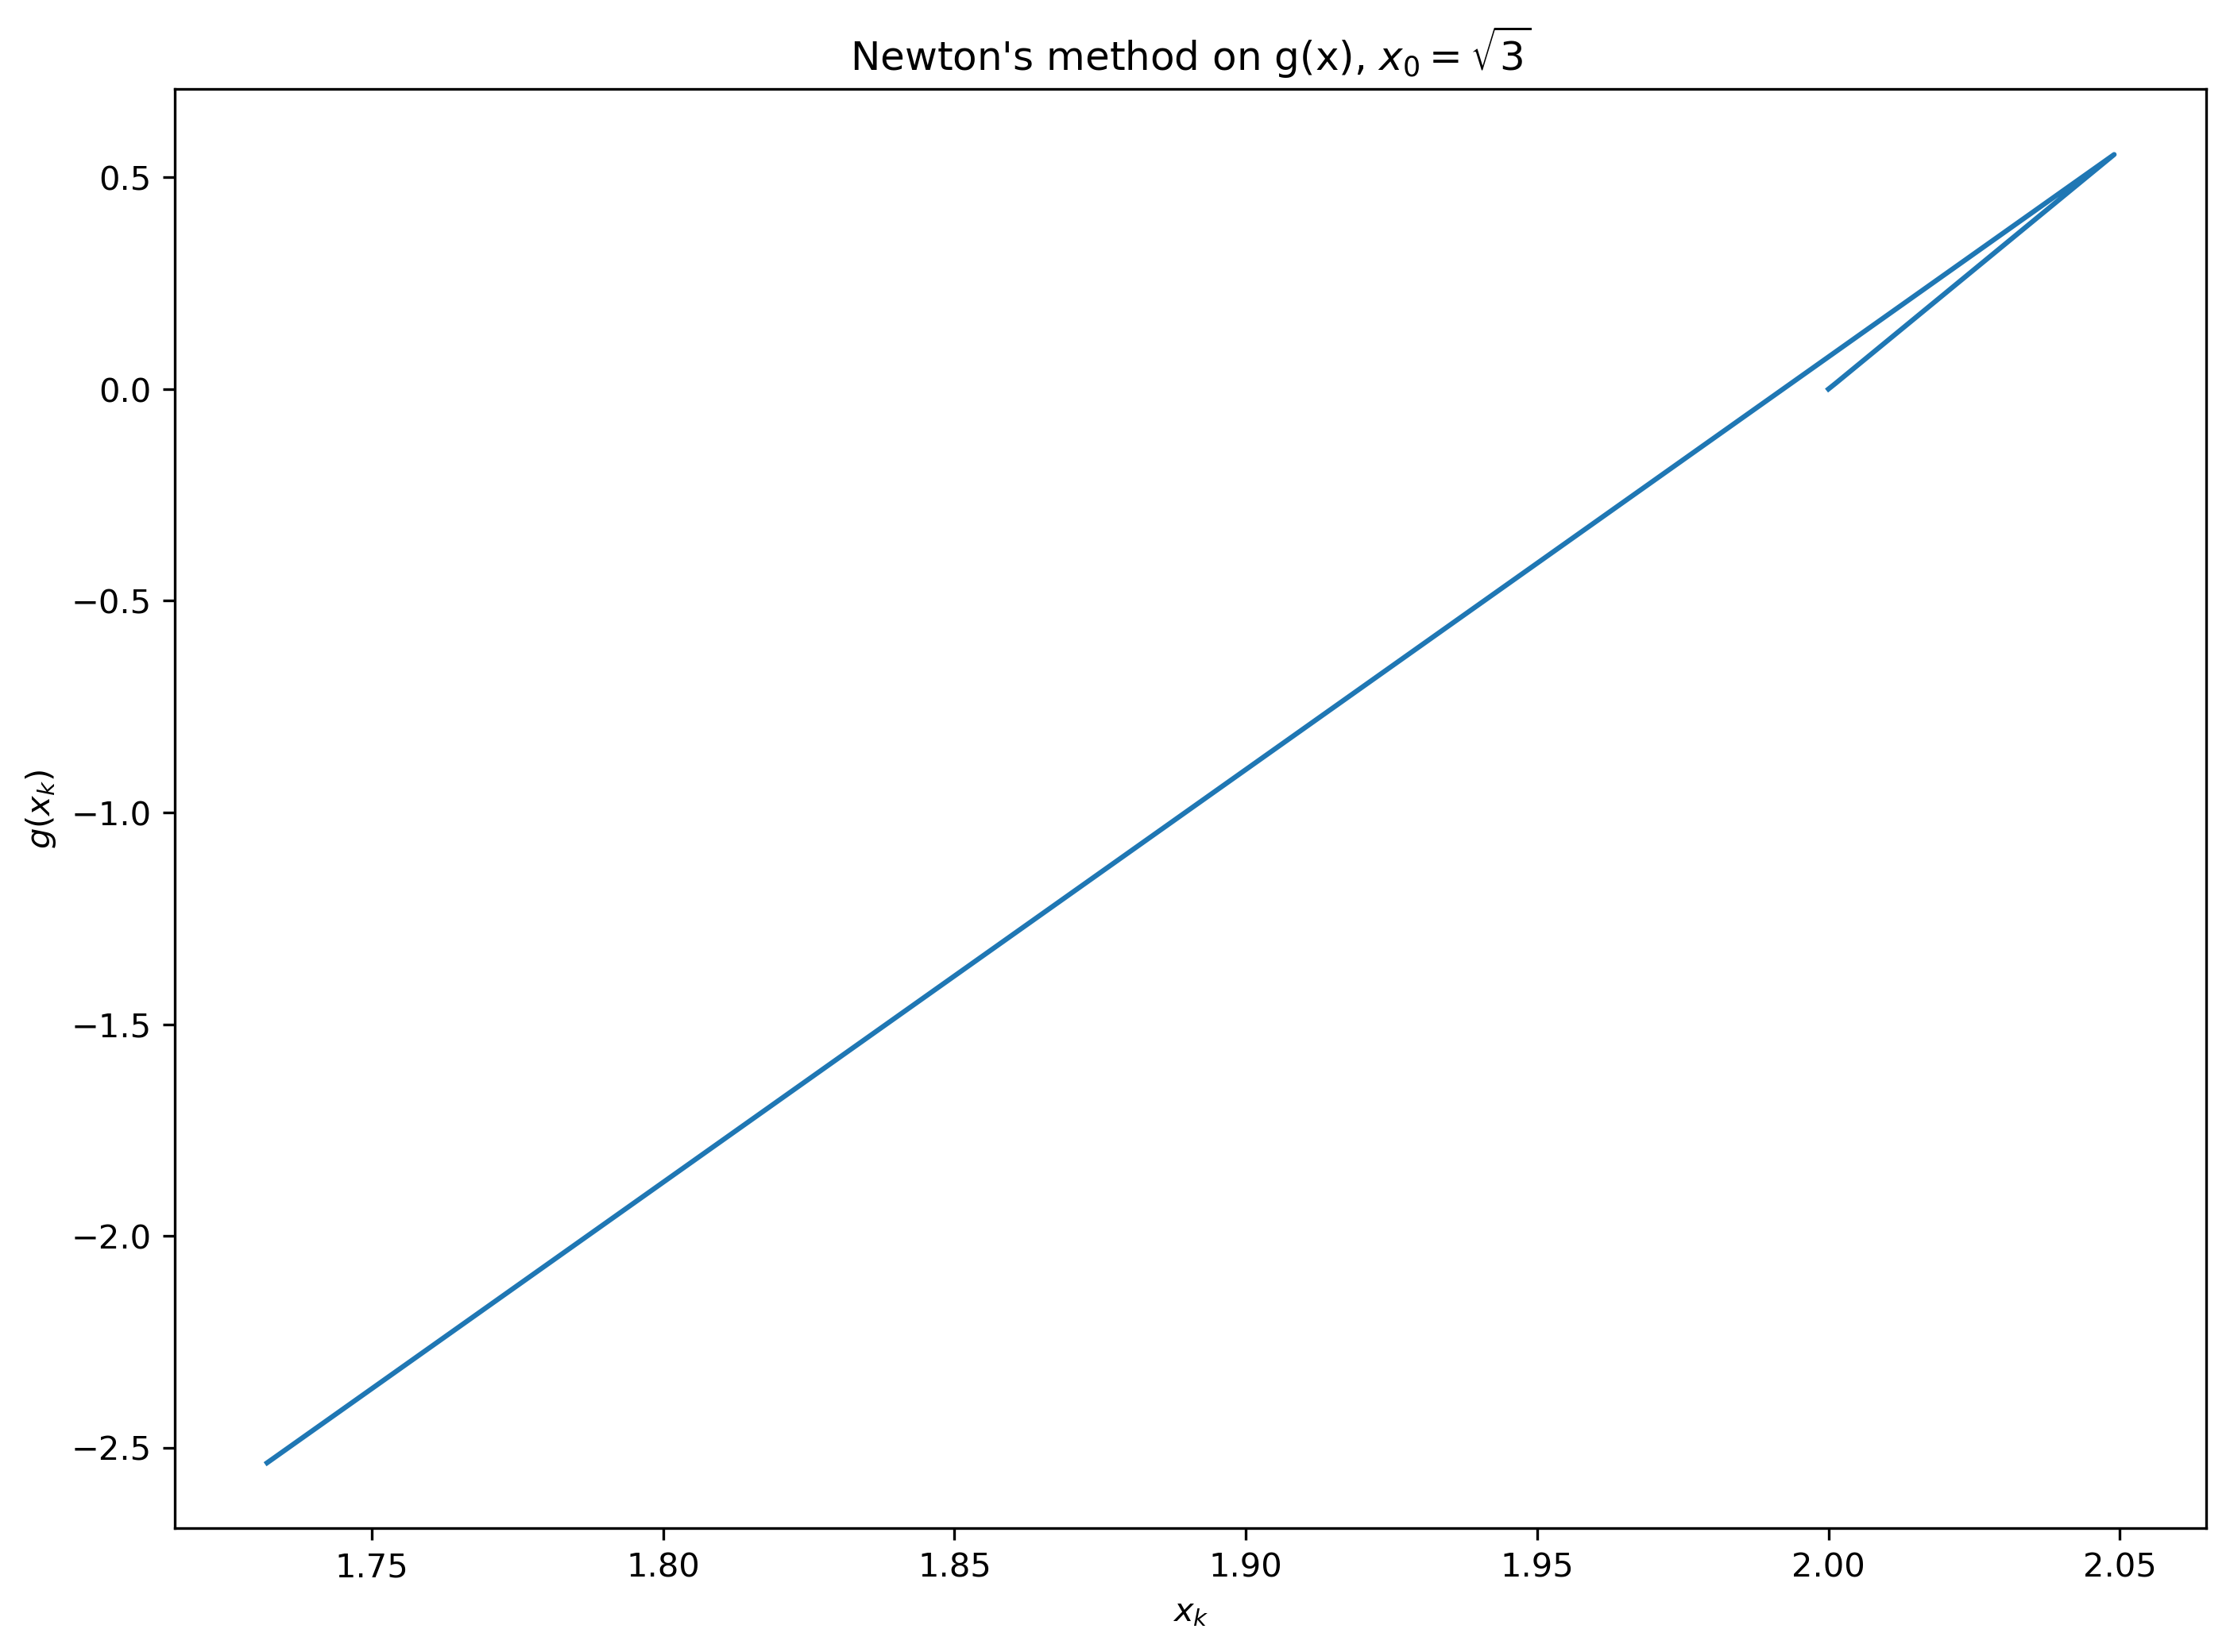
\includegraphics[width=\linewidth]{../figures/Newtons_g_sqrt3}
	\caption{Function values, $g(x_k)$, versus $x_k$ for each $k$ using Newton's method with $x_0 = \sqrt{3}$.}
	\label{fig:newton_g_sqrt3}
\end{figure}

%%%%%%%%%%%%%%%%%%%%%%%%%%%%%%%%%%%%%%%%%%%%%%%%%%%%%%%%%%%%%%%%%%%%%%%%%%%%%%%%%%%

\subsection{Fixed-point Method Plots - g(x):}

\begin{figure}[H]
	\centering
	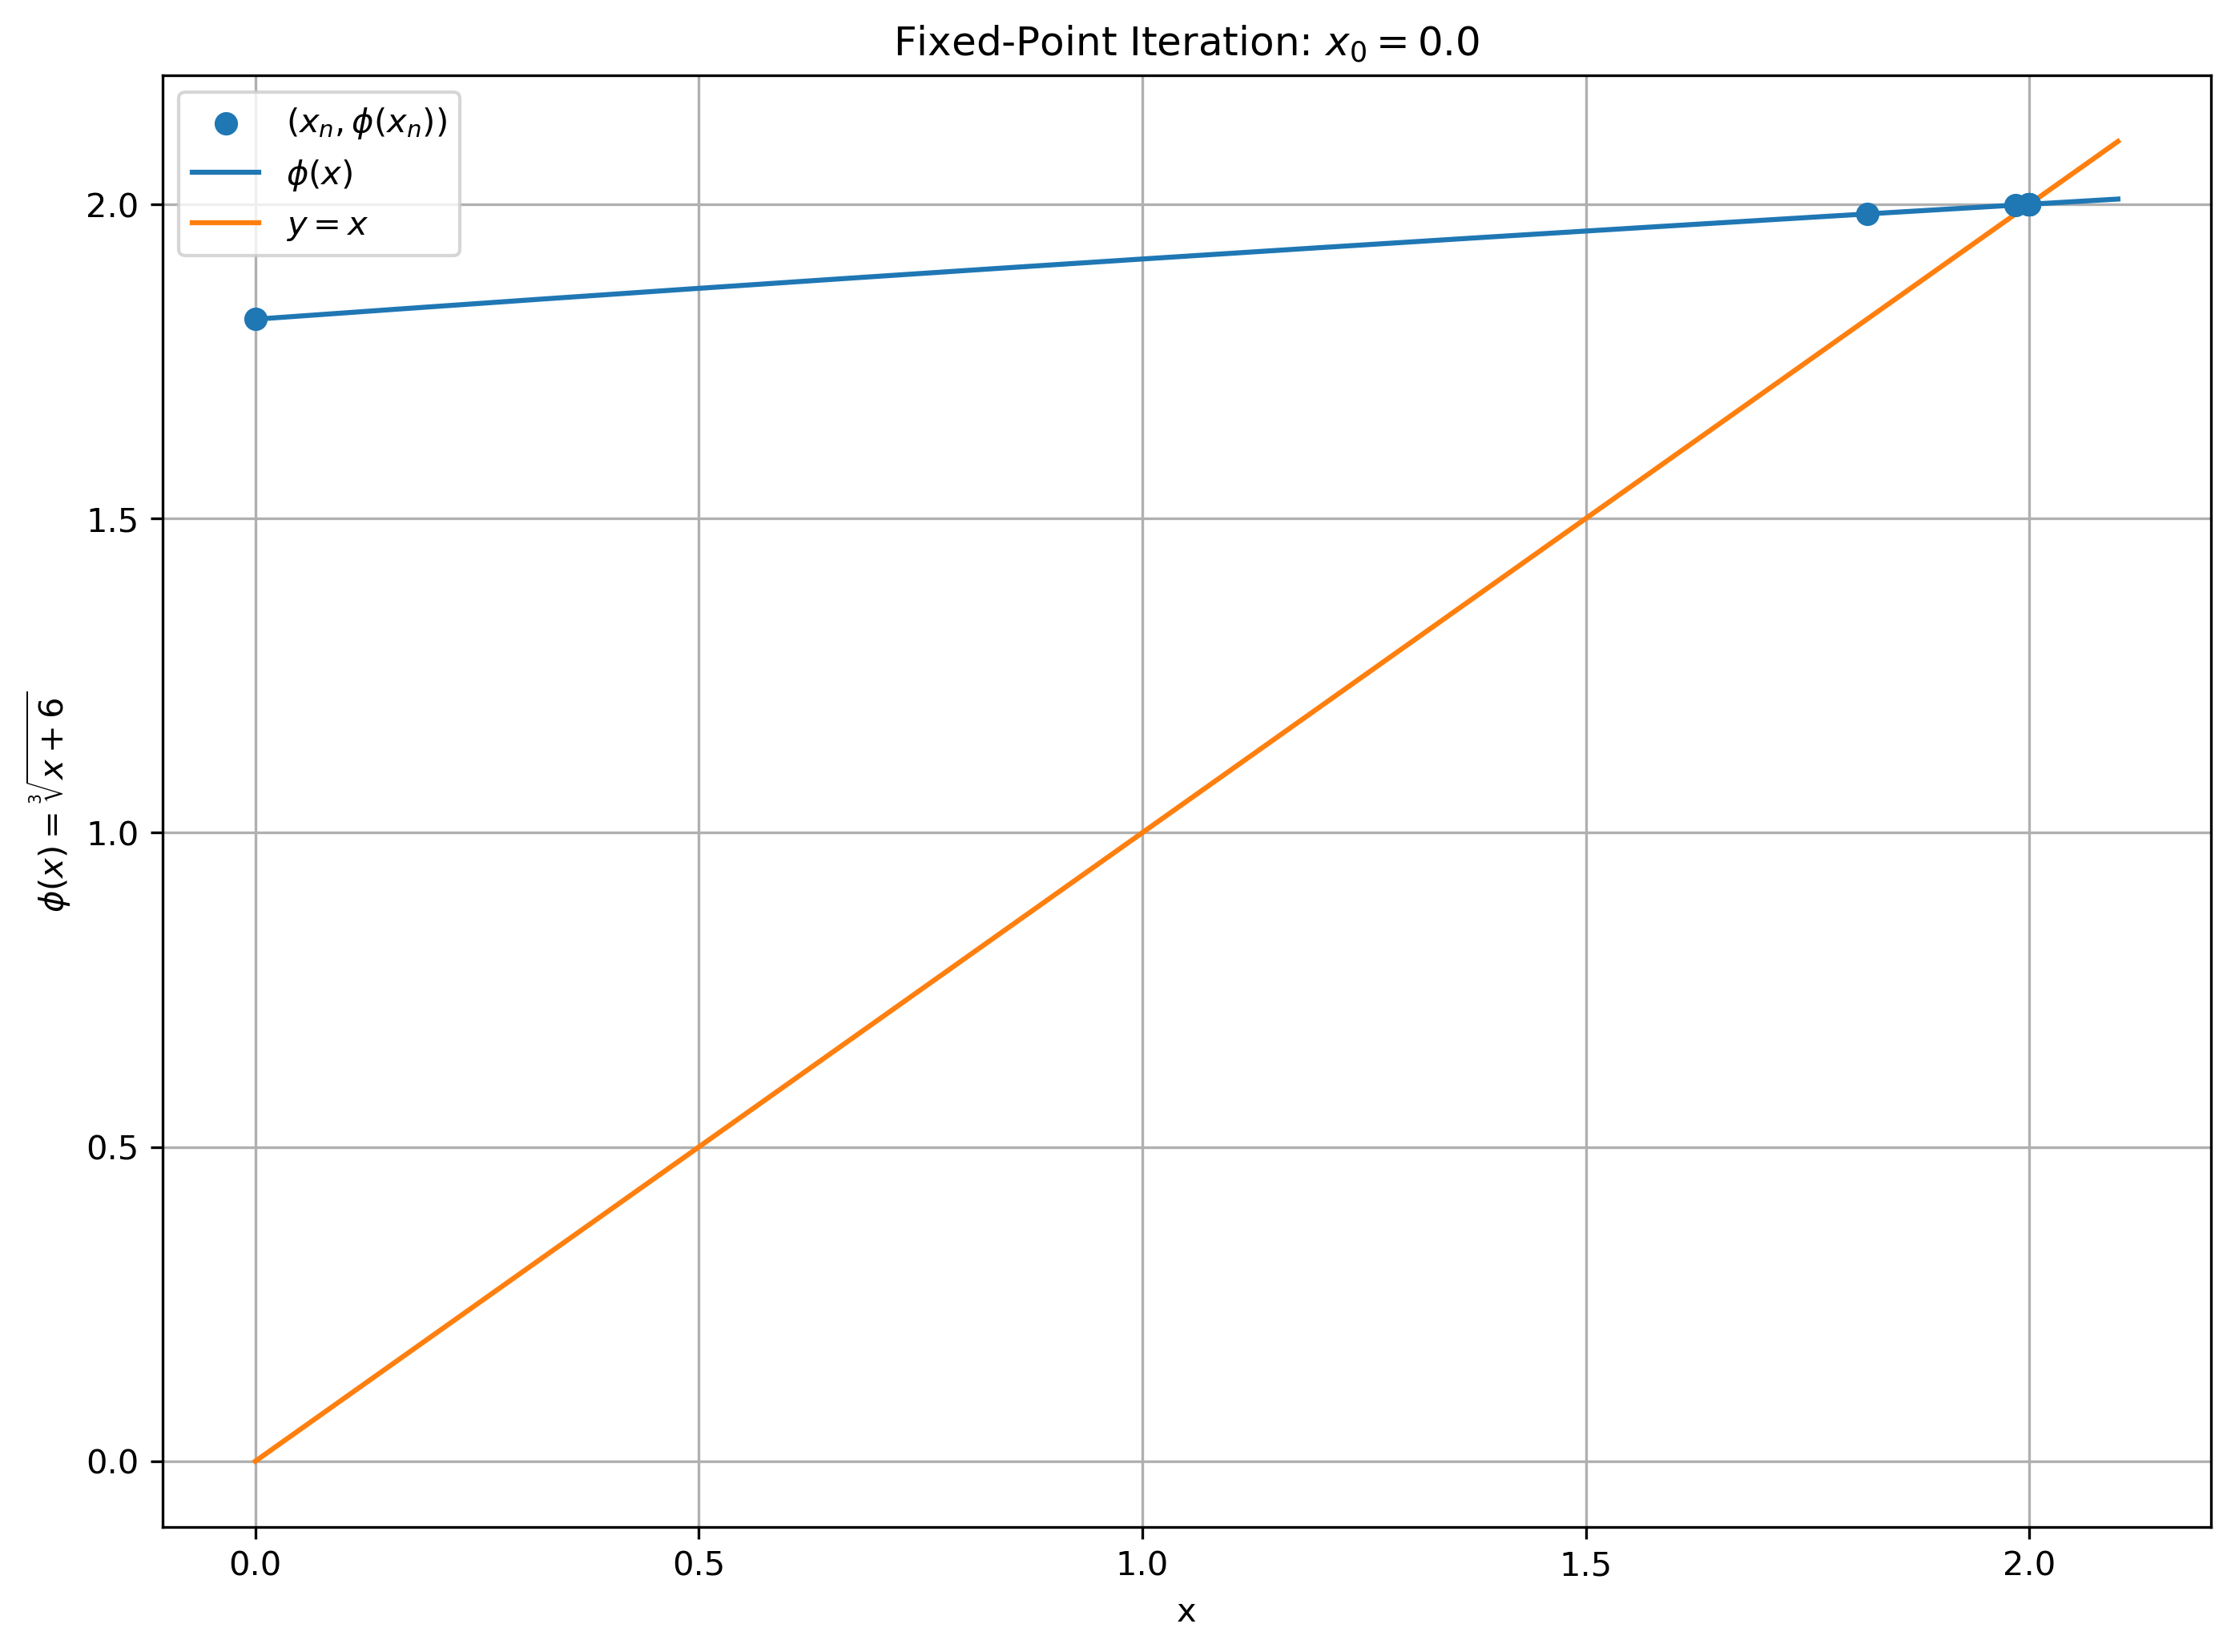
\includegraphics[width=\linewidth]{../figures/Fixed_g}
	\caption{Fixed-point function values, $\phi(x_k)$, versus $x_k$ for each $k$ using fixed-point method with $x_0 = 0.0$.}
	\label{fig:fixed_g_0.0}
\end{figure}

%%%%%%%%%%%%%%%%%%%%%%%%%%%%%%%%%%%%%%%%%%%%%%%%%%%%%%%%%%%%%%%%%%%%%%%%%%%%%%%%%%%
%%%%%%%%%%%%%%%%%%%%%%%%%%%%%%%%%%%%%%%%%%%%%%%%%%%%%%%%%%%%%%%%%%%%%%%%%%%%%%%%%%%

\subsection{Bisection Method Plots - Correctness Test:}
\begin{figure}[H]
	\centering
	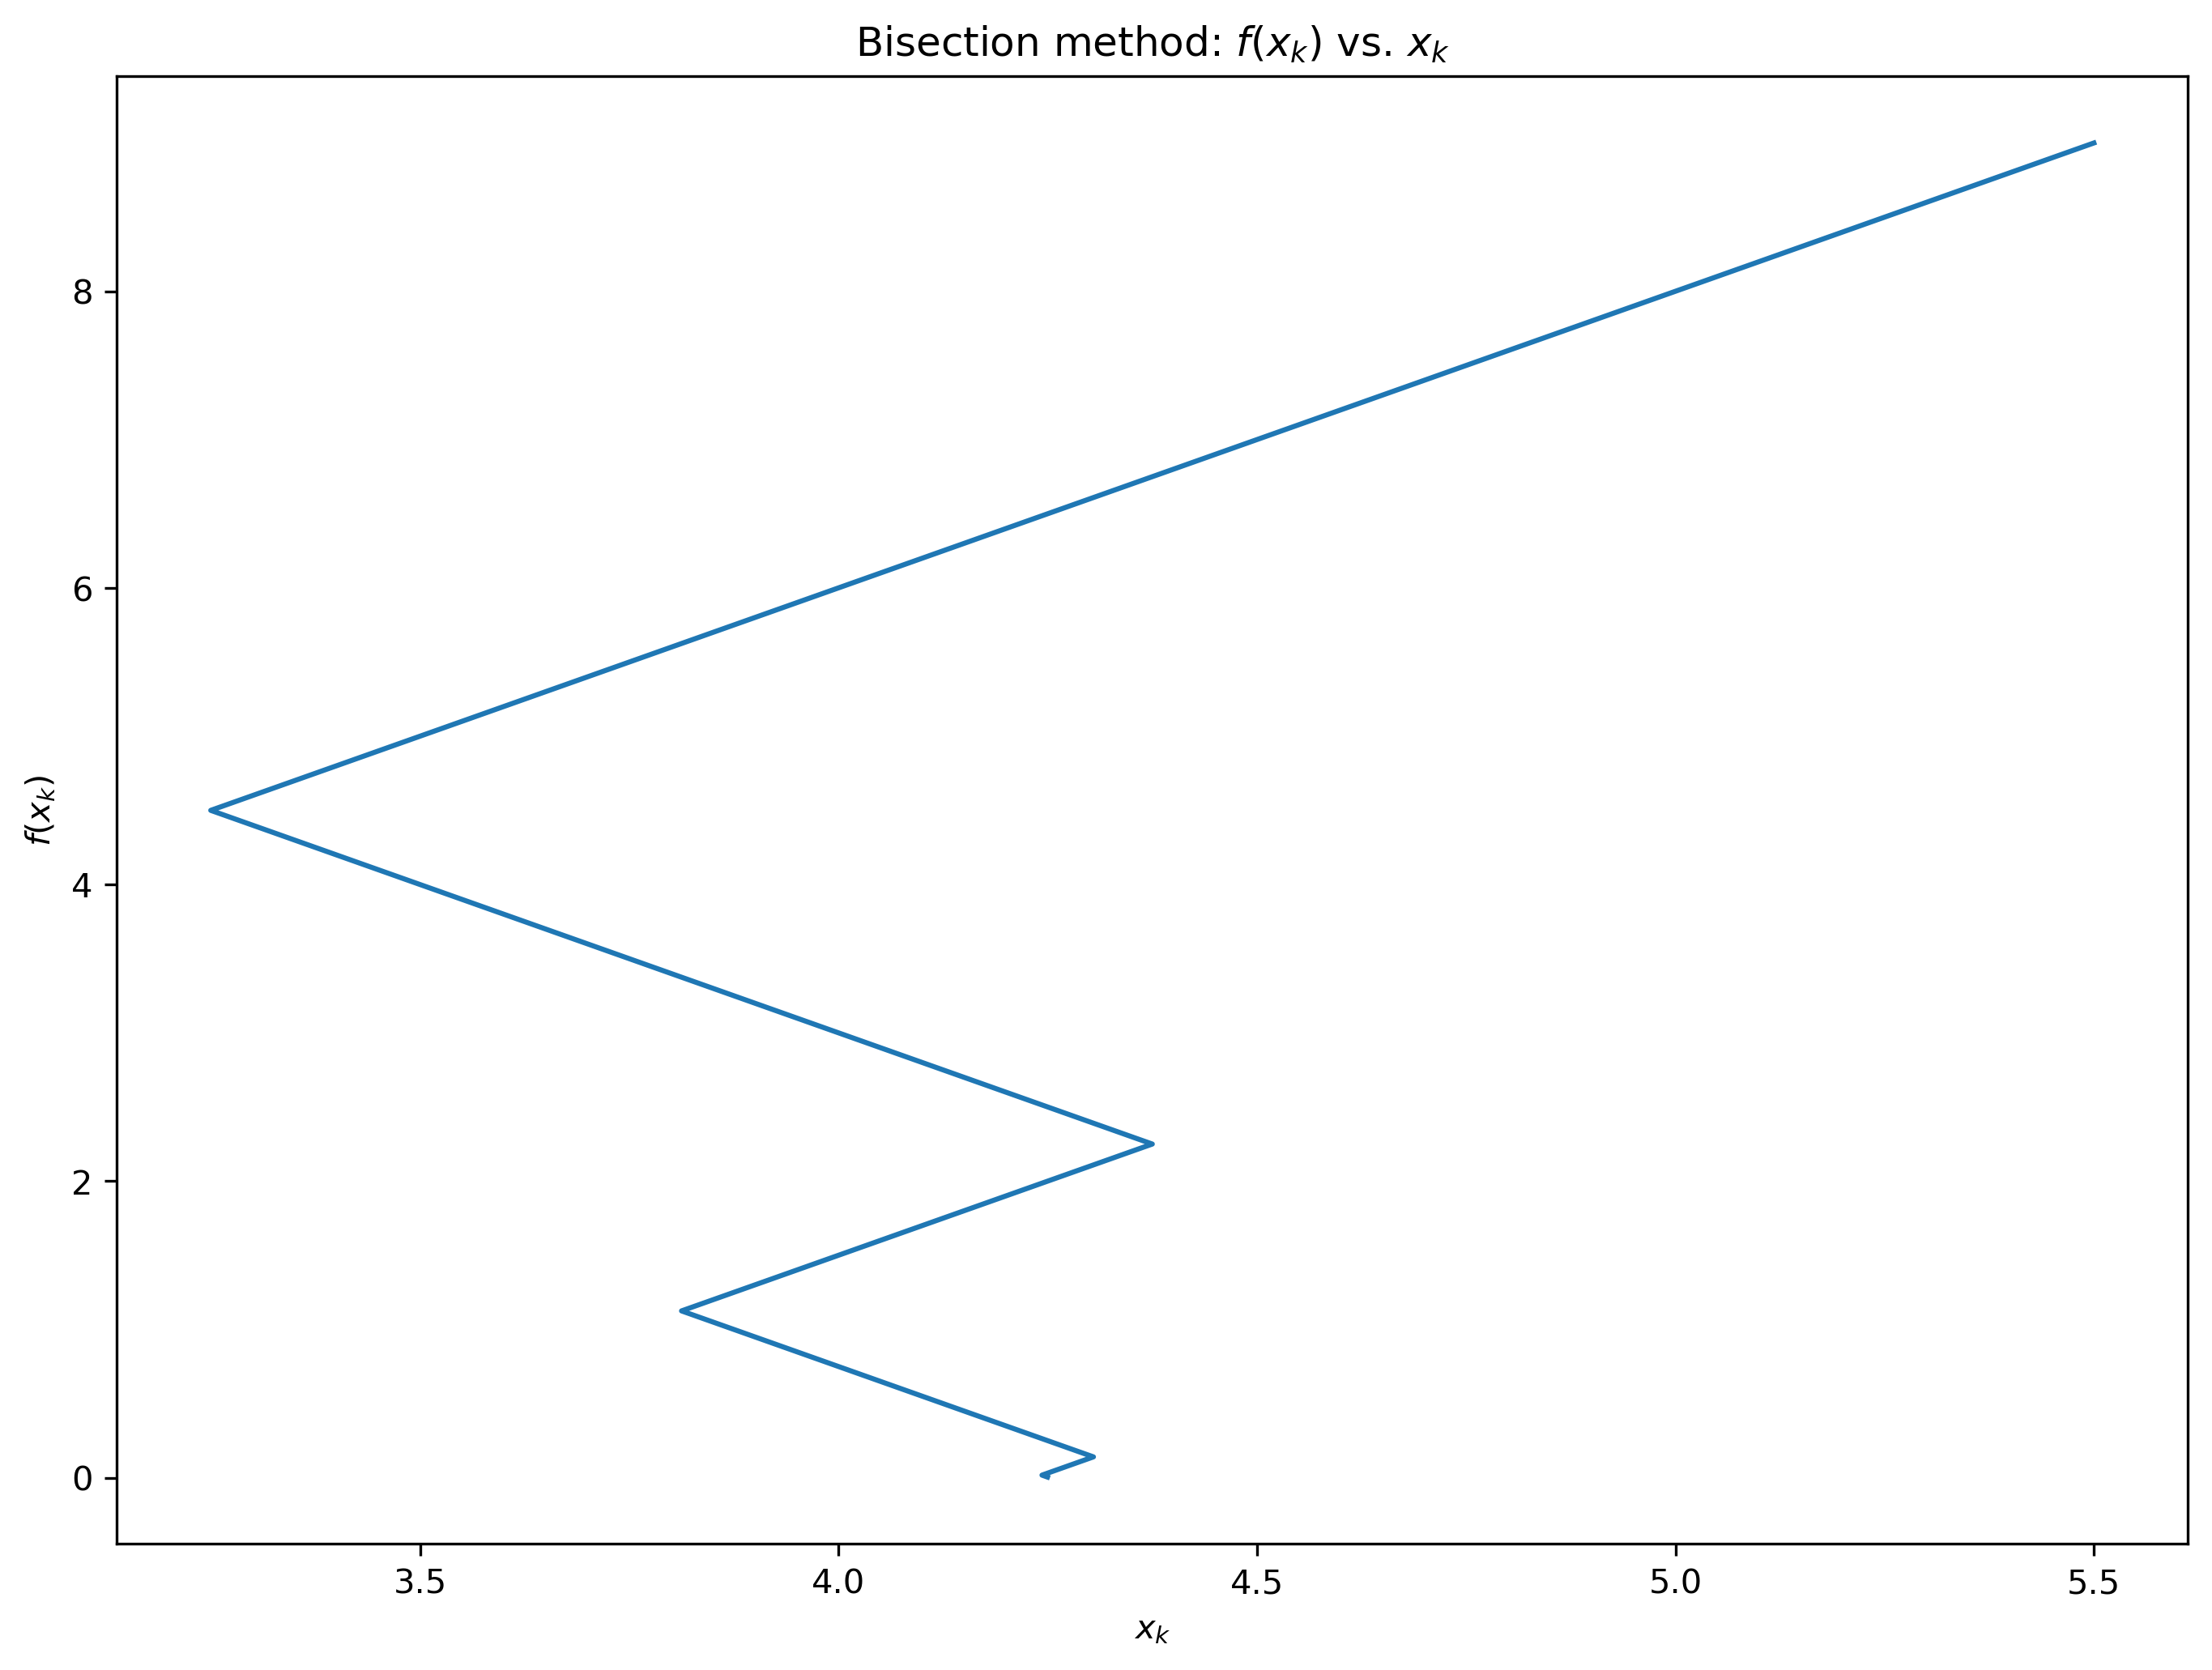
\includegraphics[width=\linewidth]{../figures/Bisection_Test}
	\caption{Function values, $f(x_k)$, versus $x_k$ for each $k$ using the bisection method with starting interval $[a,b]= [1,10]$.}
	\label{fig:bisec_test}
\end{figure}

\subsection{Newton's Method Plots - Correctness Test:}
\begin{figure}[H]
	\centering
	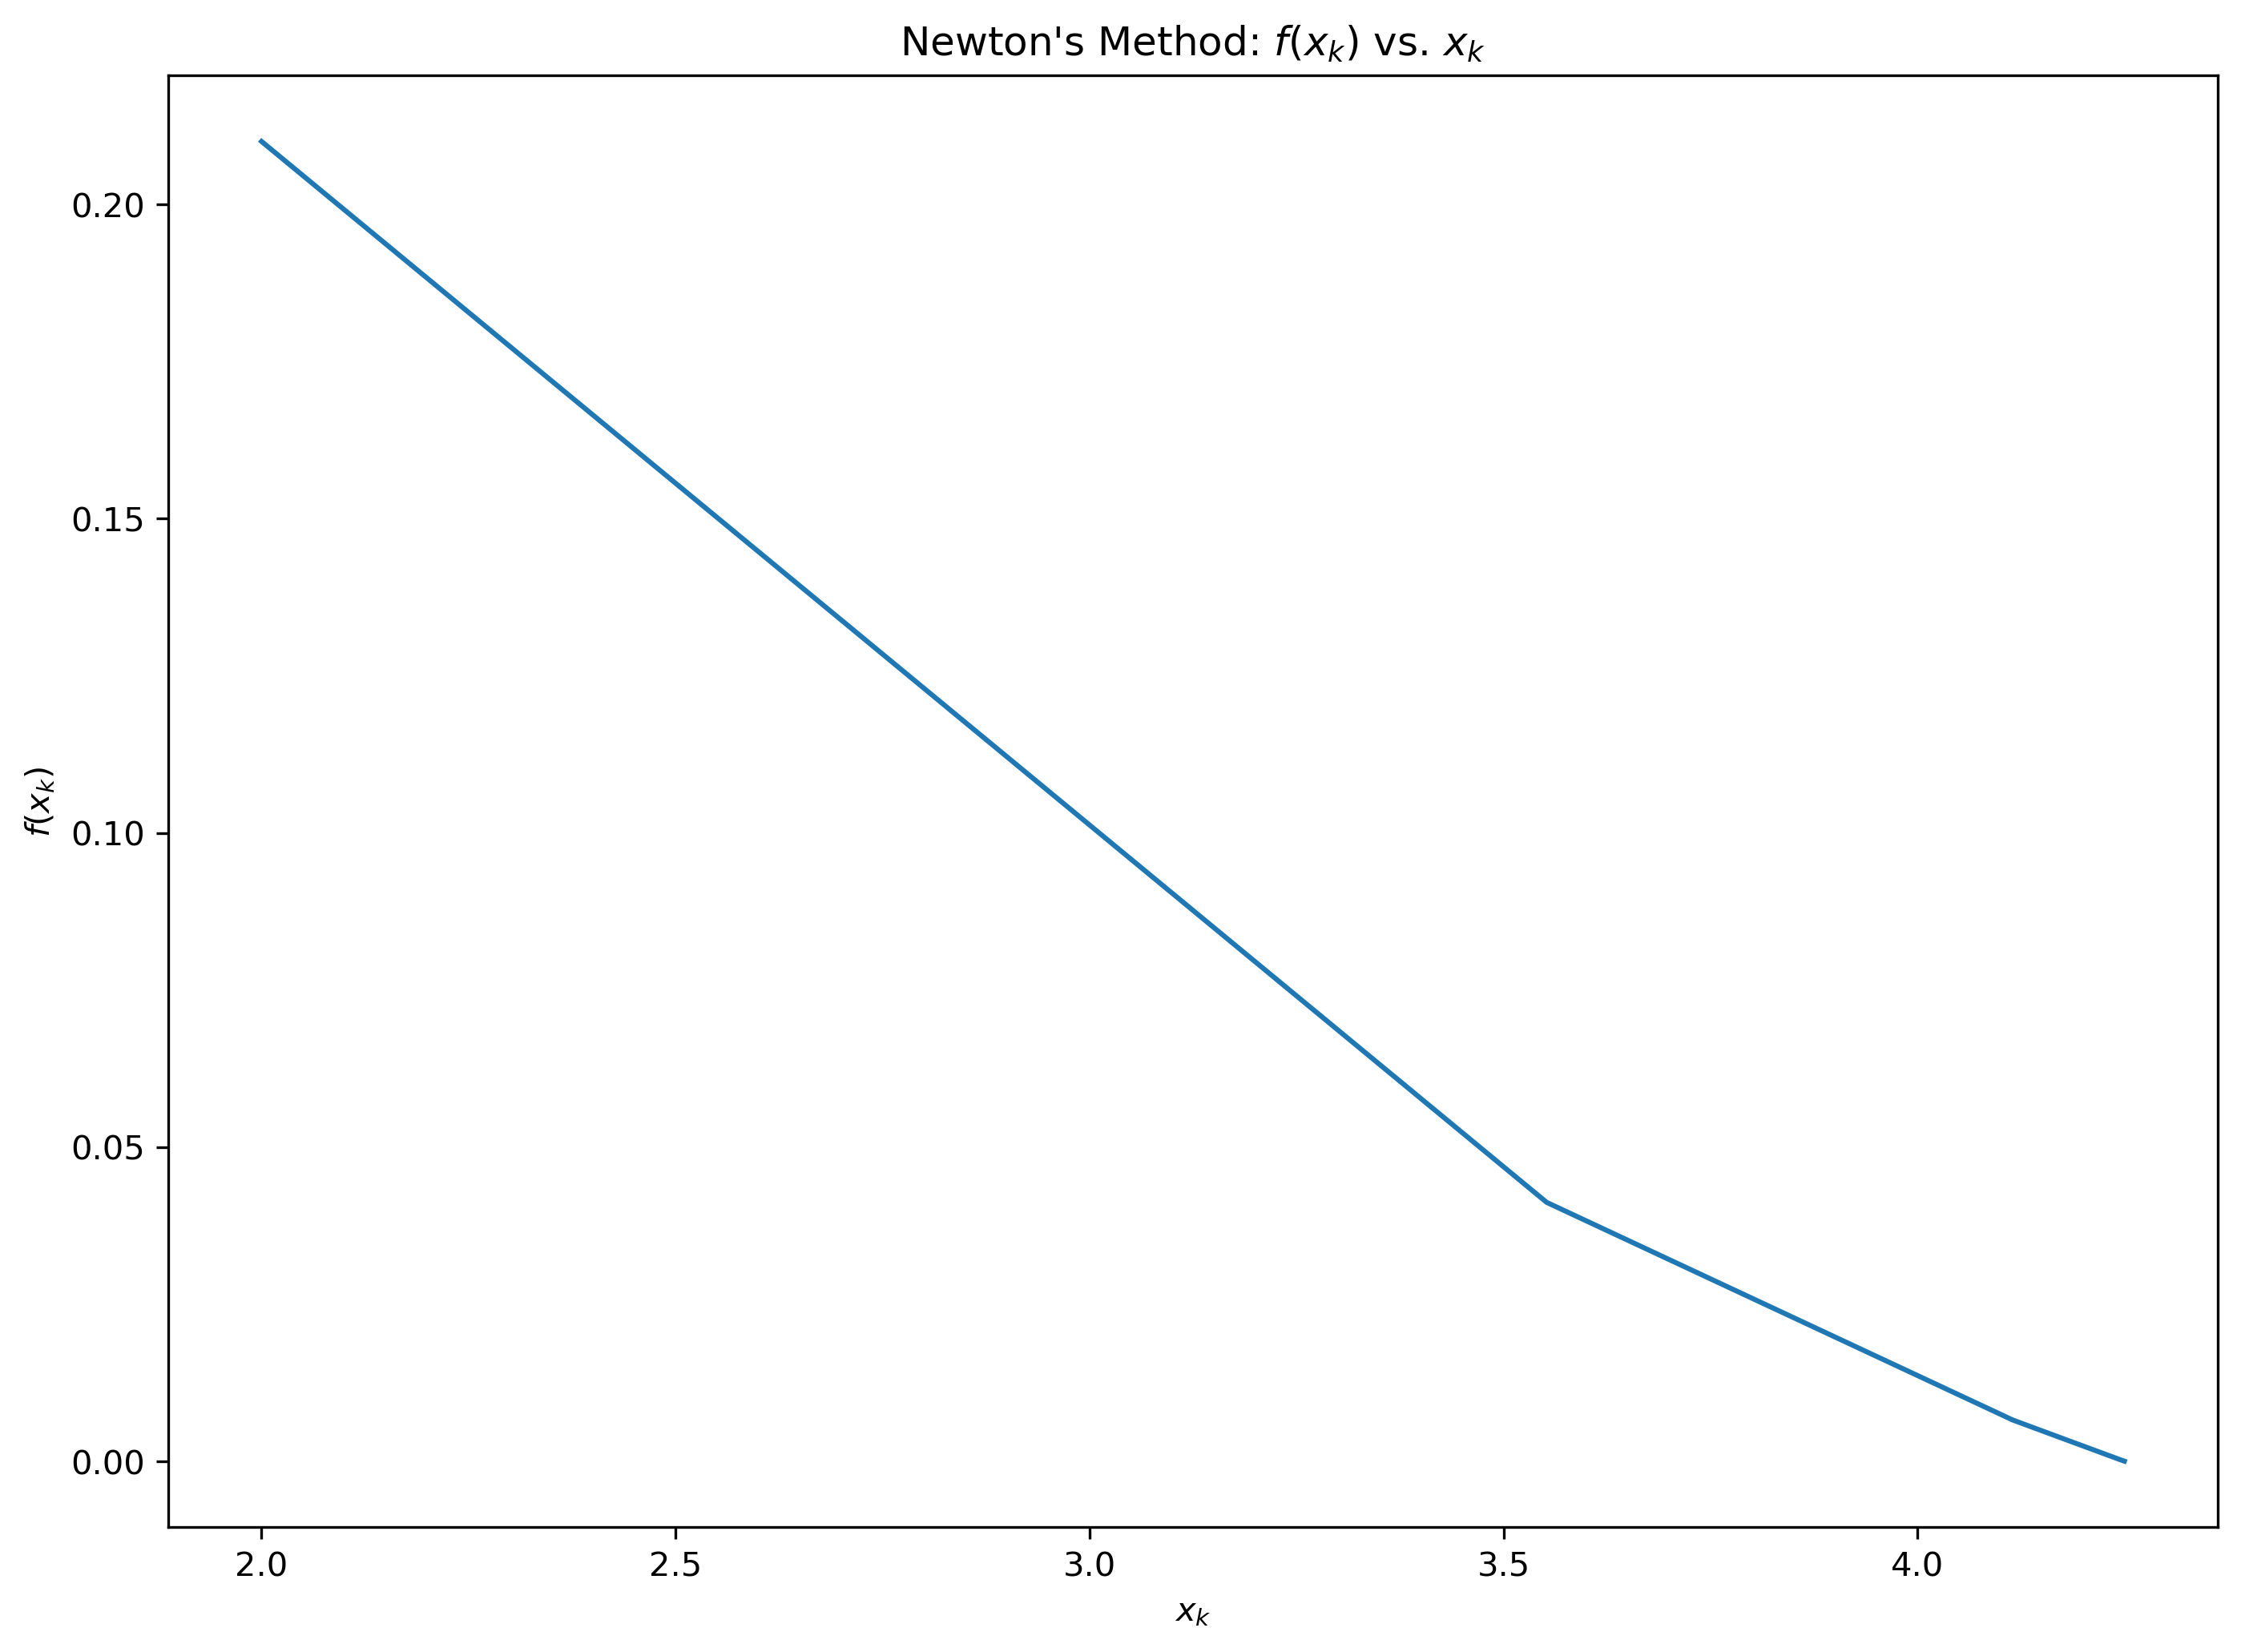
\includegraphics[width=\linewidth]{../figures/Newtons_Test}
	\caption{Function values, $f(x_k)$, versus $x_k$ for each $k$ using Newton's method with starting value $x_0 = 2$.}
	\label{fig:newtons_test}
\end{figure}

\subsection{Fixed-point Method Plots - Correctness Test:}
\begin{figure}[H]
	\centering
	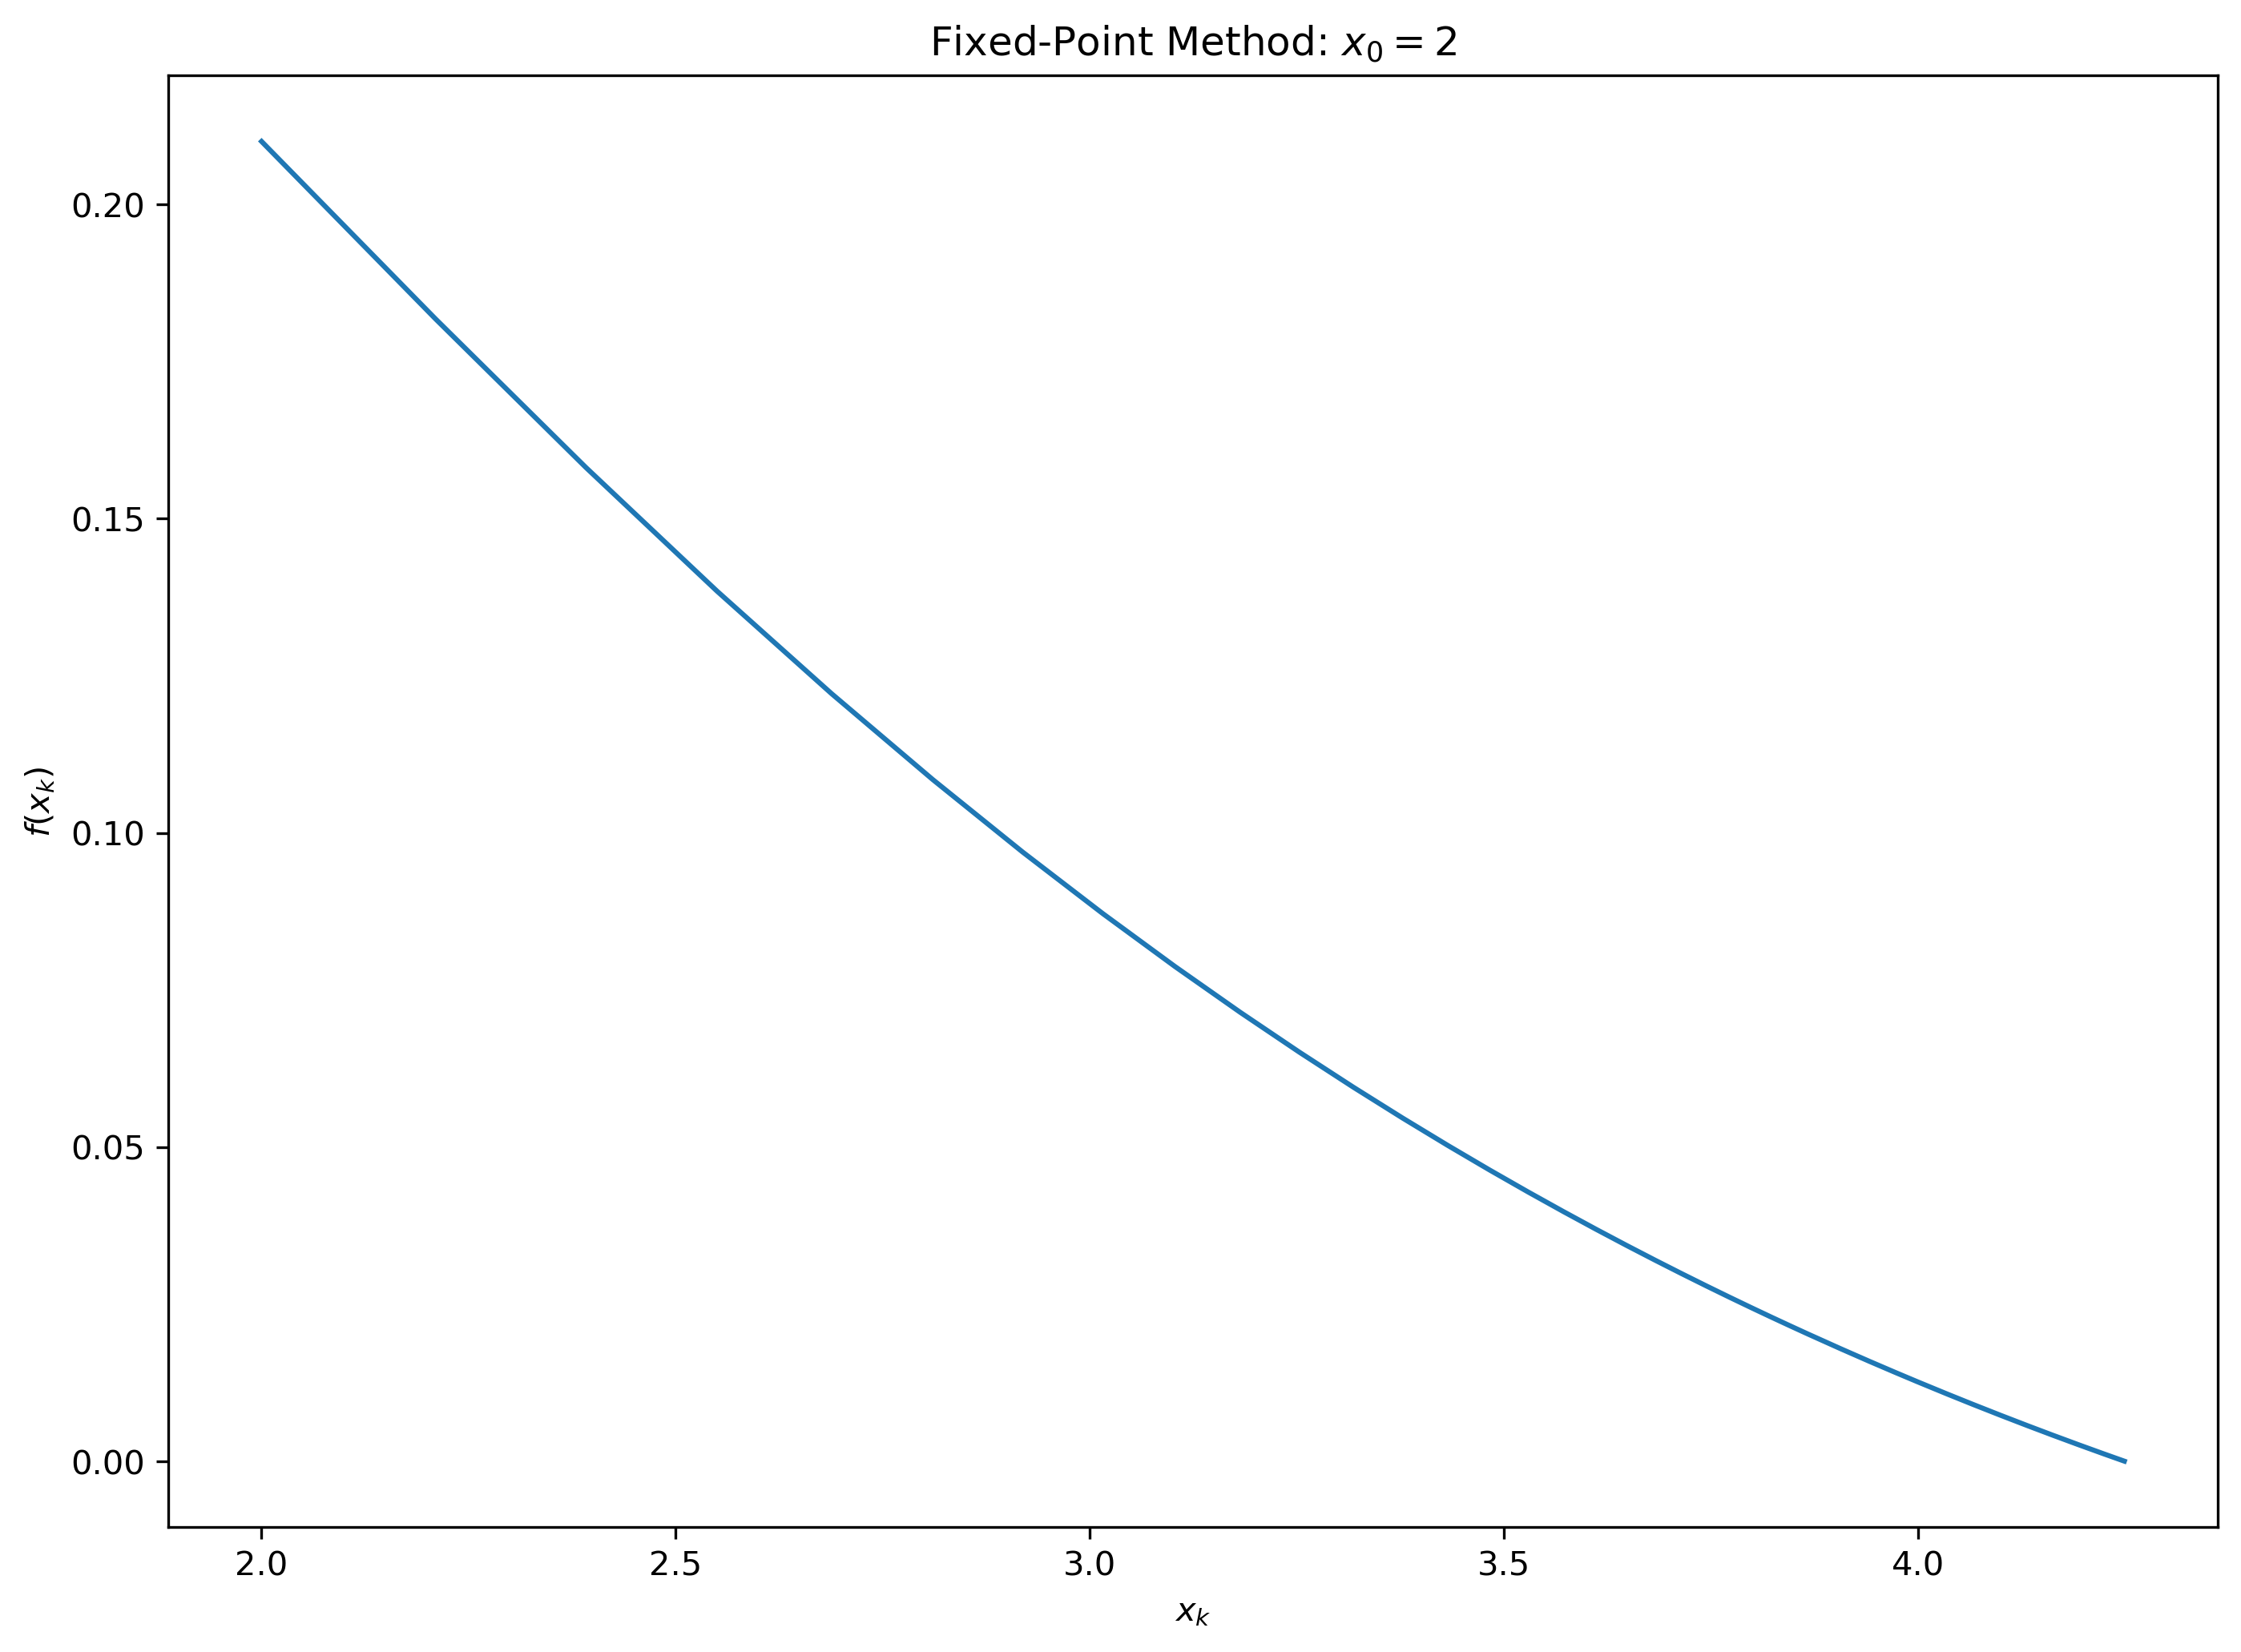
\includegraphics[width=\linewidth]{../figures/Fixed_Test_fx}
	\caption{Function values, $f(x_k)$, versus $x_k$ for each $k$ using fixed-point method with starting value $x_0 = 2$.}
	\label{fig:fixed_test}
\end{figure}


\clearpage
%%%%%%%%%%%%%%%%%%%%%%%%%%%%%%%%%%%%%%%%%%%%%%%%%%%%%%%%%%%%%%%%%%%%%%%%%%%%%%%%%%%
%%%%%%%%%%%%%%%%%%%%%%%%%%%%%%%%%%%%%%%%%%%%%%%%%%%%%%%%%%%%%%%%%%%%%%%%%%%%%%%%%%%
%%%%%%%%%%%%%%%%%%%%%%%%%%%%%%%%%%%%%%%%%%%%%%%%%%%%%%%%%%%%%%%%%%%%%%%%%%%%%%%%%%%

\begin{table}[h!]
	\centering
	\begin{tabular}{ccc}
		\hline
		\multicolumn{3}{|c|}				{Bisection Method - f(x)}                                            \\ \hline
		\multicolumn{1}{|c|}{Interval [a,b]} & \multicolumn{1}{c|}{Root} & \multicolumn{1}{c|}{Iterations} \\ \hline
		\multicolumn{1}{|c|}{[0,1]}  & \multicolumn{1}{c|}	{0.064693} & \multicolumn{1}{c|}     {18} \\ \hline
		\multicolumn{1}{|c|}{[1,7]}  & \multicolumn{1}{c|}	{4.249618} & \multicolumn{1}{c|}     {18} \\ \hline
		\multicolumn{1}{|c|}{[1,10]} & \multicolumn{1}{c|}	{4.249756} & \multicolumn{1}{c|}     {12} \\ \hline
	\end{tabular}
	\caption{Roots calculated (column 2) and iterations taken (column 1) of the bisection method on $f(x) = xe^{-x} - 0.06064$ with the given intervals (column 1).}
	\label{tab:bisec_f}
\end{table}

\begin{table}[h!]
	\centering
	\begin{tabular}{|cc|}
		\hline
		\multicolumn{2}{|c|}	{Bisection Method - g(x)}      \\ \hline
		\multicolumn{1}{|c|}{Interval [a, b]} & [1, 10]    \\ \hline
		\multicolumn{1}{|c|}{Root}            & 1.99999994 \\ \hline
		\multicolumn{1}{|c|}{Iterations}      & 24         \\ \hline
	\end{tabular}
	\caption{Root calculated (row 3) and iterations taken (row 4) of the bisection method on $g(x) = x^3 - x - 6$ with the given interval (row 1).}
	\label{tab:bisec_g}
\end{table}

\begin{table}[h!]
	\centering
	\begin{tabular}{|ccc|}
		\hline
		\multicolumn{3}{|c|}		{Newton's Method - f(x)}                                       \\ \hline
		\multicolumn{1}{|c|}{Initial $x_0$} & \multicolumn{1}{c|}{Root}       & Iterations \\ \hline
		\multicolumn{1}{|c|}{1.0}           & \multicolumn{1}{c|}{N/A}        & N/A        \\ \hline
		\multicolumn{1}{|c|}{0.99}          & \multicolumn{1}{c|}{0.06469251} & 92         \\ \hline
		\multicolumn{1}{|c|}{0.0}           & \multicolumn{1}{c|}{0.06469263} & 4          \\ \hline
		\multicolumn{1}{|c|}{1.1}           & \multicolumn{1}{c|}{0.06469214} & 191        \\ \hline
		\multicolumn{1}{|c|}{2.0}           & \multicolumn{1}{c|}{4.249621}   & 5        \\ \hline
		\multicolumn{1}{|c|}{4.0}           & \multicolumn{1}{c|}{4.249633}   & 4          \\ \hline
		\multicolumn{1}{|c|}{6.0}           & \multicolumn{1}{c|}{4.249626}   & 6          \\ \hline
	\end{tabular}
	\caption{Roots calculated (column 2) and iterations taken (column 3) of Newton's method on $f(x) = xe^{-x} - 0.06064$ with the given starting value, $x_0$, (column 1).}
	\label{tab:newton_f}
\end{table}

\begin{table}[h!]
	\centering
	\begin{tabular}{|ccc|}
		\hline
		\multicolumn{3}{|c|}		{Newton's Method - g(x)}                                         \\ \hline
		\multicolumn{1}{|c|}{Initial $x_0$}        & \multicolumn{1}{c|}{Root}  & Iterations \\ \hline
		\multicolumn{1}{|c|}{1/$\sqrt{3}$} & \multicolumn{1}{c|}{N/A}   & N/A        \\ \hline
		\multicolumn{1}{|c|}{0.57735}              & \multicolumn{1}{c|}{2.000} & 47         \\ \hline
		\multicolumn{1}{|c|}{1.0}                  & \multicolumn{1}{c|}{2.000} & 7          \\ \hline
		\multicolumn{1}{|c|}{0.0}                  & \multicolumn{1}{c|}{2.000} & 32         \\ \hline
		\multicolumn{1}{|c|}{$\sqrt{3}$}           & \multicolumn{1}{c|}{2.000} & 5          \\ \hline
	\end{tabular}
	\caption{Roots calculated (column 2) and iterations taken (column 3) of Newton's method on $g(x) = x^3 - x - 6$ with the given starting value, $x_0$, (column 1).}
	\label{tab:newton_g}
\end{table}

\begin{table}[h!]
	\centering
	\begin{tabular}{|ccc|}
		\hline
		\multicolumn{3}{|c|}		{Fixed-Point Method - f(x)}                                   \\ \hline
		\multicolumn{1}{|c|}{Initial $x_0$} & \multicolumn{1}{c|}{Root}      & Iterations \\ \hline
		\multicolumn{1}{|c|}{0.0}           & \multicolumn{1}{c|}{0.0646926} & 7          \\ \hline
		\multicolumn{1}{|c|}{2.0}           & \multicolumn{1}{c|}{4.249430} & 183          \\ \hline
		\multicolumn{1}{|c|}{4.5}           & \multicolumn{1}{c|}{4.2496333} & 11         \\ \hline
	\end{tabular}
	\caption{Roots calculated (column 2) and iterations taken (column 3) of the fixed-point method on $f(x) = xe^{-x} - 0.06064$ with the given starting value, $x_0$, (column 1).}
	\label{tab:fixed_f}
\end{table}

\begin{table}[h!]
	\centering
	\begin{tabular}{|ccc|}
		\hline
		\multicolumn{3}{|c|}{Fixed-Point Method - g(x)}                               \\ \hline
		\multicolumn{1}{|c|}{Initial $x_0$} & \multicolumn{1}{c|}{Root}  & Iterations \\ \hline
		\multicolumn{1}{|c|}{0.0}           & \multicolumn{1}{c|}{2.000} & 8          \\ \hline
	\end{tabular}
	\caption{Root calculated (column 2) and iterations taken (column 3) of the Fixed-point method on $g(x) = x^3 - x - 6$ with the given starting value, $x_0$, (column 1).}
	\label{tab:fixed_g}
\end{table}

\end{document}
